
% Szkielet dla pracy pisanej w języku polskim.

\documentclass[polish,a4paper,twoside,bachelor, 10pt]{ppfcmthesis}

\usepackage[utf8]{inputenc}
\usepackage[OT4]{fontenc}
\usepackage{listings}

\author{Krzysztof Figiel}                              % Your name comes here
\title{Analiza działania i bezpieczeństwa aplikacji WWW opartych na języku JavaScript z wykorzystaniem nowoczesnych technologii implementacji warstwy prezentacji.

Security and functioning analisys of applications based on JavaScript language with the use of modern frontend technologies.}                   % Note how we protect the final title phrase from breaking
\ppsupervisor{dr inż. Izabela Janicka-Lipska } % Your supervisor comes here.
\ppyear{2018}                                         % Year of final submission (not graduation!)

\begin{document}

% Front matter starts here
\frontmatter\pagestyle{empty}%
\maketitle\cleardoublepage%

% Blank info page for "karta dyplomowa"
\thispagestyle{empty}\vspace*{\fill}%
\begin{center}
	\begin{figure}[h]
		\centering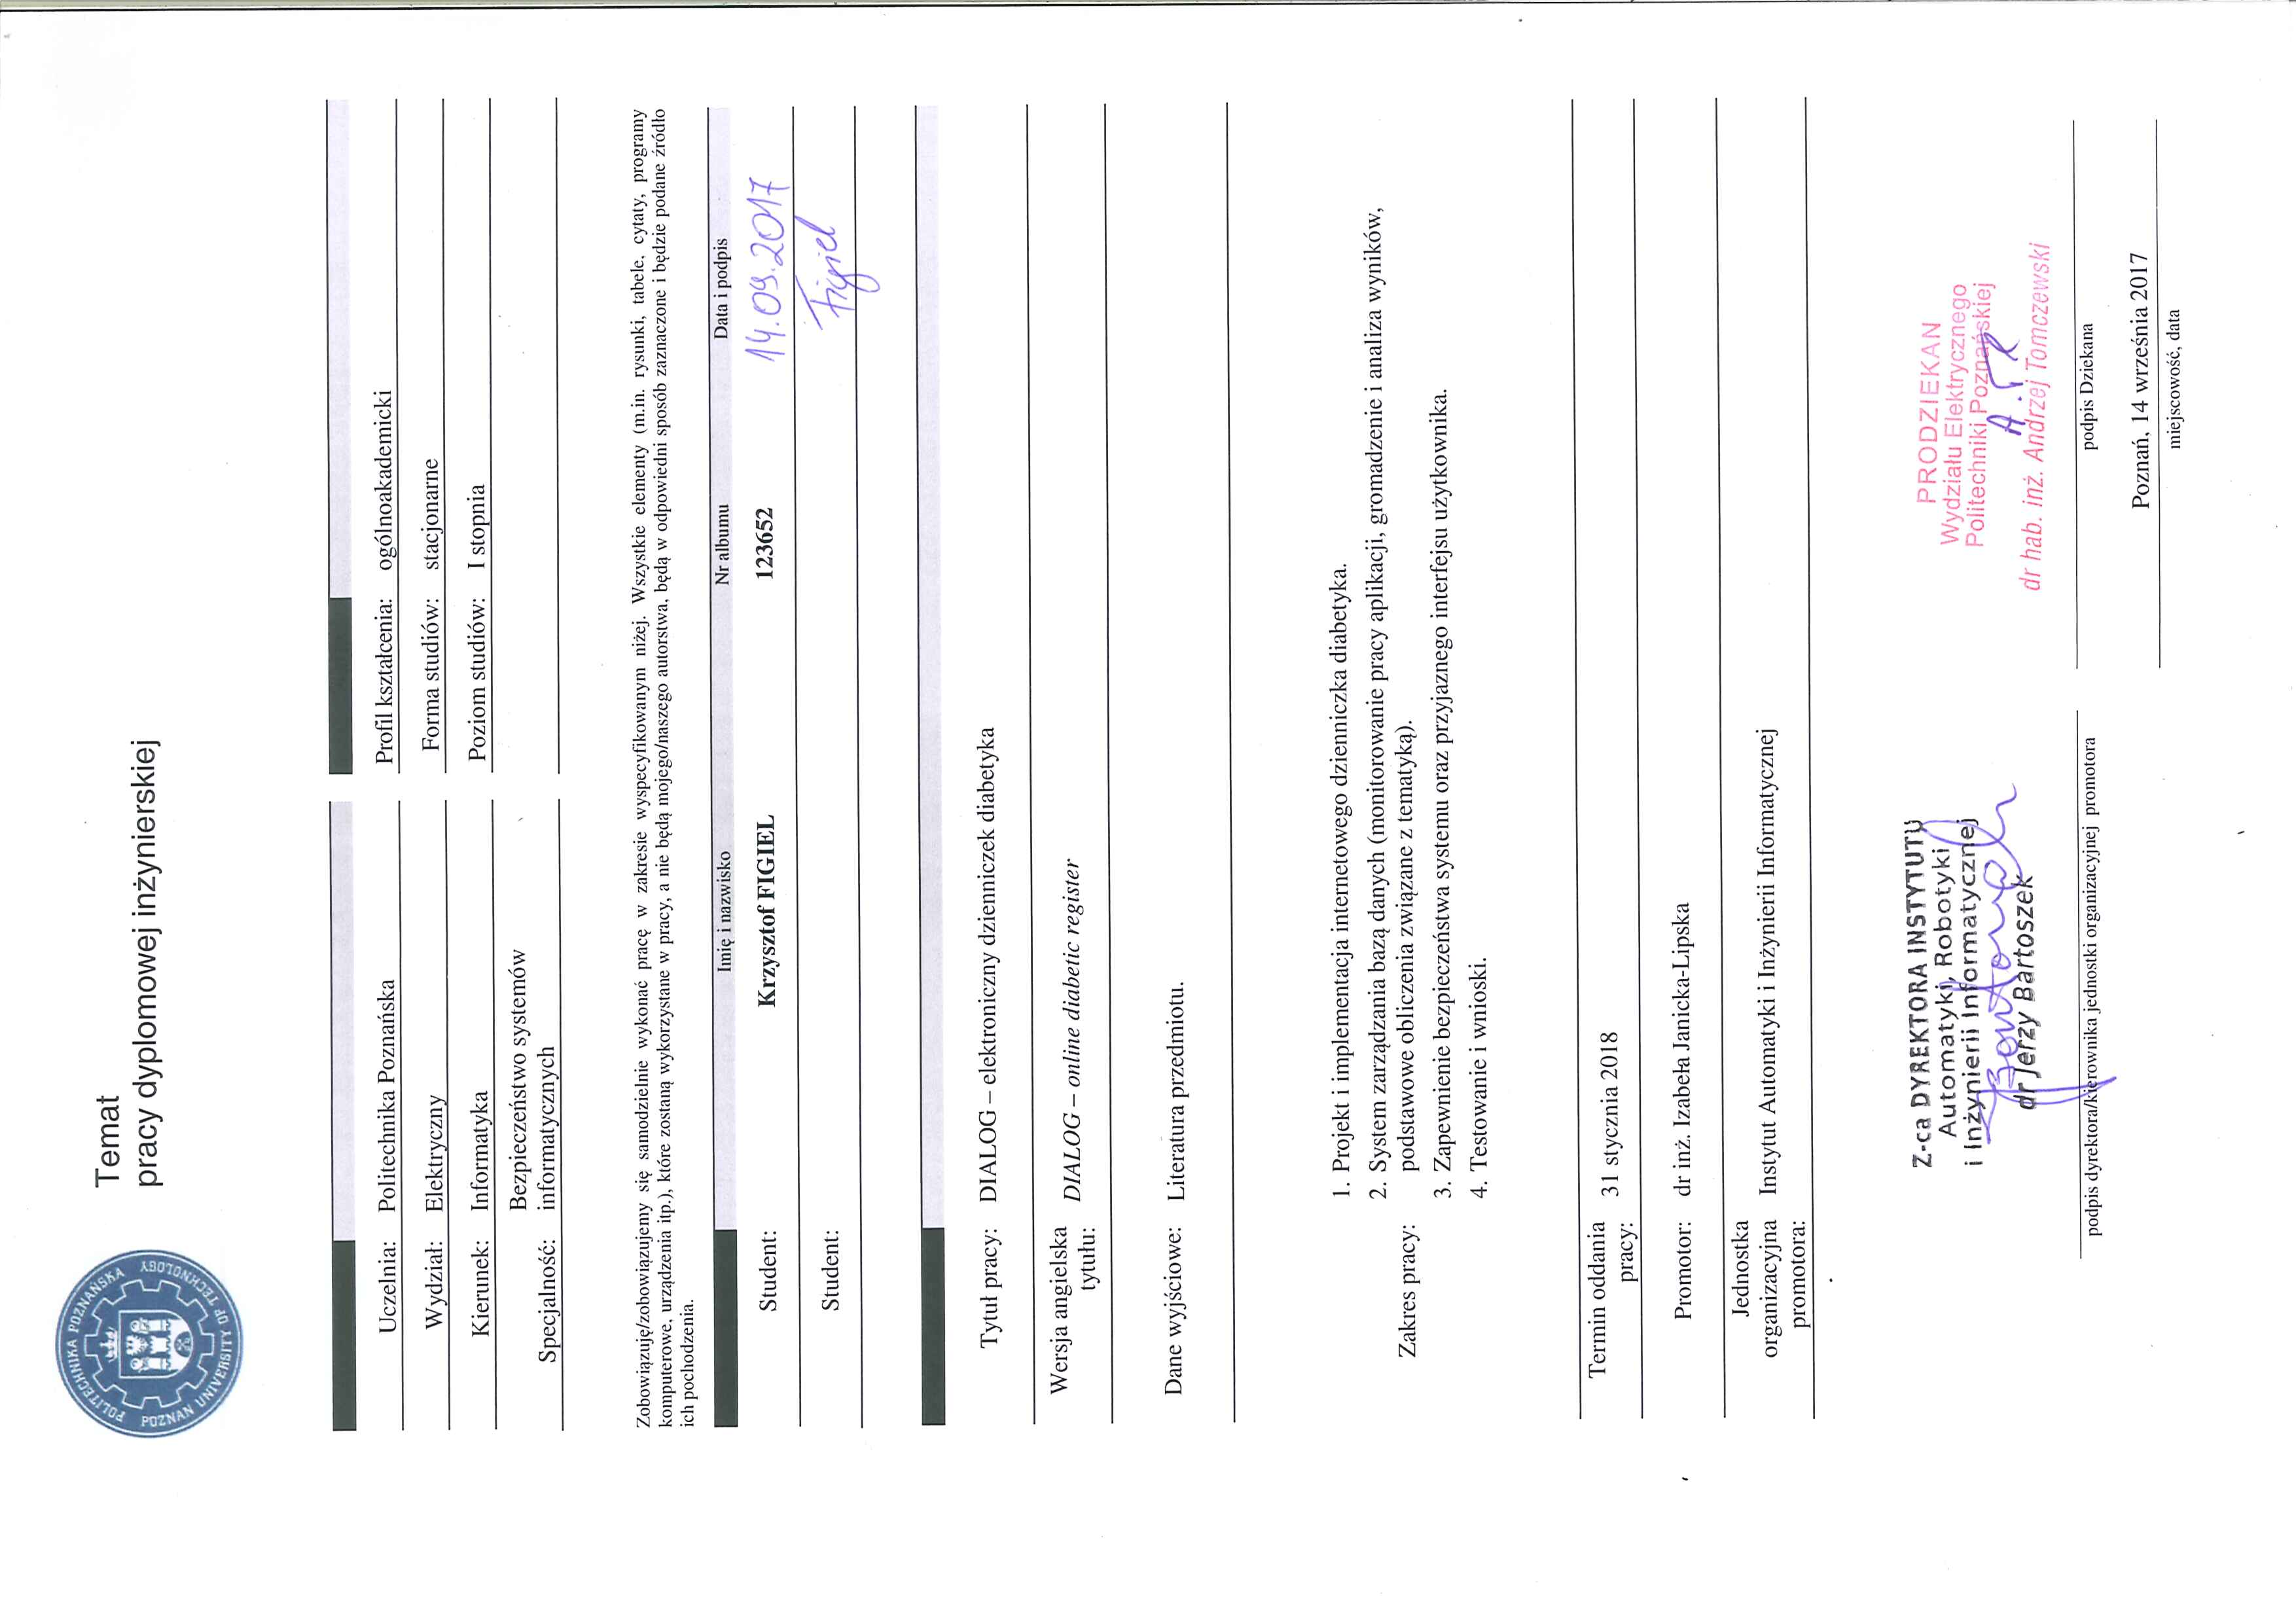
\includegraphics[angle=270, scale=0.73]{images/karta_pracy.jpg}
	\end{figure}
\end{center}%
\vfill\cleardoublepage%

\section*{\fontsize{16}{1}\selectfont Streszczenie}
Za cel pracy postawiono omówienie oraz analizę działania i bezpieczeństwa aplikacji WWW opartych na języku \textit{JavaScript} z wykorzystaniem nowoczesnych technologii implementacji warstwy prezentacji takich jak \textit{Angular}, hybrydowa technologia \textit{Ionic}, framework \textit{React} czy \textit{Vue.js}. W celu lepszego poznania odpowiednich bibliotek i wzorców projektowych z nimi powiązanych posłużono się dokumentacjami technicznymi poszczególnych zestawów narzędzi. Przeanalizowano mechanizmy bezpieczeństwa oferowane przez frameworki. Wykorzystano autorskie implementacje kluczowych fragmentów funkcjonowania aplikacji internetowych i na ich podstawie zestawiono i omówiono otrzymane wyniki i wnioski. 

\section*{\fontsize{16}{1}\selectfont Abstract}
The main aim of this graduation work is to discuss and analyze the functionality and security of WWW applications based on \textit{JavaScript} language using modern frontend technologies like \textit{Angular}, hybrid framework \textit{Ionic}, \textit{React} and \textit{Vue.js}. For better understanding each of the technologies technical documentation was used. The security mechanisms offered by each framework were analyzed in depth. Authors implementations of key fragments of the functioning of WWW applications were used. The obtained results anc conclusions were summarized and discussed. 

\vfill\cleardoublepage%

% Table of contents.
\pagenumbering{Roman}\pagestyle{ppfcmthesis}%
\tableofcontents* \cleardoublepage%

% Main content of your thesis starts here.
\mainmatter%

\chapter{Wstęp}

%Wstęp\footnote{Treść przykładowych rozdziałów została skopiowana
%z ,,zasad'' redakcji prac dyplomowych FCMu~\cite{fcm-red}.} do pracy powinien zawierać następujące elementy:
\section{Wprowadzenie}
Wybór tematu pracy magisterskiej spowodowany był chęcią udoskonalenia i poszerzenia swojej wiedzy na temat tworzenia nowoczesnych aplikacji WWW opartych na języku \textit{JavaScript} z wykorzystaniem technologii implementacji warstwy prezentacji oraz mechanizmów bezpieczeństwa z nimi powiązanych. Aktualny rynek pracy i ciagły rozwój technologii informatycznych (zwłaszcza tych internetowych) powodują stałe udoskonalanie aktualnych rozwiązań technologicznych, a co za tym idzie uodparnianie ich na problemy związane z bezpiecznym przechowywaniem danych. Kolejnym argumentem, który wskazuje na mój wybór jest fakt, że aktualnie pracuję na stanowisku web dewelopera, tak więc tworzenie bezpiecznych aplikacji internetowych jest zarówno źródłem mojego dochodu, jak i zainteresowań. W dzisiejszych czasach programista ma dostęp do wielu użytecznych bibliotek i rozwiązań, które w znacznym stopniu ułatwiają implementację najważniejszych mechanizmów komunikacji poszczególnych warstw aplikacji z serwerem, dlatego też postanowiłem omówić najważniejsze z nich wraz z krótkimi implementacjami podstawowych funkcjonalności stron WWW. 

%\begin{itemize}
%    \item krótkie uzasadnienie podjęcia tematu; 
 
%\end{itemize}

\noindent

\section{Cel projektu}
Za cel projektu postawiono analizę działania i bezpieczeństwa aplikacji opartych na języku \textit{JavaScript} w oparciu o proste implementacje podstawowych funkcjonalności serwisów WWW takich jak uwierzytelnianie, formularze użytkownika czy wymiana danych między warstwami prezentacji i aplikacji. Skupiono się na zrealizowaniu podstawowych mechanizmów prewencji przeciwko atakom z poziomu warstwy aplikacji. Zaproponowano również autorskie pomysły metod dodatkowego zabezpieczania stron WWW przeciwko nieporządanemu działaniu osób trzecich. Zestawiono sposoby realizacji powyższych rozwiązań w poszczególnych technologiach frontendowych i określono, która z nich jest potencjalnie najlepsza. Ostatecznie, zaproponowano ewentualne metody ulepszeń omawianych mechanizmów i podsumowano całokształt pracy.

\section{Struktura pracy}

Praca składa się z siedmiu rozdziałów. Pierwszy z nich zawiera wprowadzenie, przedstawia cel projektu oraz ogólną strukturę pracy. W drugim opisane są technologie wykorzystane do stworzenia testowej aplikacji i analizy wybranych zagadnień. Trzeci rozdział opisuje środowisko backendowe \textit{Node.js}. Przedstawia on sposób implementacji i uruchomienia serwera z wykorzystaniem bezpiecznego połączenia - HTTPS.  Kolejny, czwarty, opisuje mechanizmy bezpieczeństwa aplikacji internetowych opartych na języku \textit{JavaScript}. W rozdziale piątym przeanalizowano i zestawiono ze sobą wybrane technologie implementacji warstwy prezentacji. Rozdział szósty zawiera analizę hybrydowego frameworka \textit{Ionic} i opisuje wybrane mechanizmy bezpieczeństwa, oferowane przez funkcje natywne biblioteki. Ostatni, siódmy rozdział jest podsumowaniem całej pracy. Na końcu znajduje się spis literatury. Do pracy dołączono załącznik w~ postaci płyty DVD. 




\chapter{Technologie}

\section{Wprowadzenie}
W poniższym rozdziale opisano najważniejsze technologie opisane w pracy. W kolejnych sekcjach przedstawiono zestaw wymagań funkcjonalnych z~podziałem na biorących udział aktorów oraz~wymagania niefunkcjonalne.

\section{Technologie}

\subsection{Framework Angular 6}
Otwarty framework stworzony przez firmę \textit{Google}, wykorzystywany do tworzenia aplikacji SPA (\textit{Single Page Application}) zarówno na platformy internetowe, jak i na natywne aplikacje mobilne i desktopowe. \textit{Angular} oparty jest na języku \textit{JavaScript} przez co zyskał on wielką popularność wśród deweloperów, w dużej mierze ze względu na swoją prostotę. Jego struktura wymusza u programistów stosowanie dobrych praktyk pisania kodu i pomaga usestymatyzować na pozór skomplikowaną architekturę aplikacji webowych. Framework ten został napisany całkowicie w mocno typowanym języku \textit{TypeScript}, który jest transpilowany do wynikowego kodu \textit{JavaScript}. \textit{Angular} swoją strukturą zachęca do budowania maksymalnie odseparowanych od siebie części kodu i komponentów. Kolejną zaletą tego frameworku jest wieloplatformowość. Pozwala on bowiem na tworzenie stron internetowych, aplikacji webowych, aplikacji PWA (\textit{Progressive Web Application}), aplikacji mobilnych z użyciem bibliotek takich jak \textit{Cordova} czy też aplikacji desktopowych mogących odnosić się do funkcji systemu i lokalnych urządzeń. Wersja szósta frameworka \textit{Angular} wprowadza zmiany m.in. w rejestrowaniu serwisów, stosowaniu \textit{RxJS}, walidacji formularzy czy w komendach CLI (\textit{Command Line Interface}).
 
\subsection{TypeScript 3}
\textit{TypeScript} jest językiem kompilowanym do języka \textit{JavaScript}, który urchamiany jest w dowolnej przeglądarce, na serwerze \textit{Node.js} czy w innym silniku, który wspiera \textit{ECMAScript} w wersji trzeciej lub nowszej. Jest to język silnie i statycznie typowany, który pomaga deweloperom stosować dobre, programistyczne praktyki. Statyczne typowanie rozumiane jest przez to, że zmienne w tym języku mają nadane typy, które nie mogą ulec zmianie. Silne typowanie wprowadza nie tylko przejrzystość kodu i jego lepsze debugowanie, ale również takie możliwości jak \textit{IntelliSense}, czyli podpowiedzi. Zastosowanie \textit{TypeScript} pozwala pozbyć się przypadkowych błędów związanych z niepewnością odnośnie typów danych oraz eliminuje problemy związane ze skalowalnością. Umożliwia stosowanie interfejsów, które pozwalają podnieść poziom abstrakcji i uzyskać luźniejsze powiązania pomiędzy klasami w aplikacjach.

\subsection{HTML5}
HTML5 (\textit{HyperText Markup Language}) jest najnowszą wersją popularnego standardu opisującego język HTML. W stosunku do poprzedników zawiera on nowe elementy, atrybuty i zachowania. Pozwala na bardziej różnorodne tworzenie stron i aplikacji internetowych. Umożliwia nowoczesną komunikację z serwerem, pozwala stronom internetowym na bardziej efektywne przechowywanie danych lokalnie i w trybie offline czy zapewnie większą prędkość i lepszą optymalizację w wykorzystywaniu sprzętu komputerowego. HTML5 wprowadza nowe elementy sekcji takie jak \texttt{<section>}, \texttt{<article>}, \texttt{<nav>}, \texttt{<header>} czy \texttt{<footer>}. Ulepszone zostały m.in. formularze, wymuszenie poprawności API (\textit{Application Programming Interface}) czy znaczniki \texttt{<input>} i \texttt{<output>}, które zyskały nowe atrybuty, takie jak \texttt{email} oraz \texttt{password}. HTML5 zapewnia również uproszczone odtwarzanie plików audio i wideo. Oferuje dużo prostsze tworzenie i wyświetlanie grafiki przy użyciu znaczników \texttt{<canvas>}. Ważną nowością są też tzw. \textit{Web-Workers}, które umożliwiają wielowątkową obsługę przepływu danych.

\subsection{CSS3}
CSS3 (\textit{Cascading Style Sheets}) jest to kolejna wersja kaskadowych arkuszy stylów, wprowadzająca szereg udogodnień i rozszerzająca możliwości interakcji użytkownika ze stroną internetową. W porównaniu do poprzednich wersji, zmiany w CSS3 obejmują między innymi zastosowanie animowanych elementów czy wszelkiego rodzaju efektów graficznych, takich jak gradienty oraz cienie. 
CSS3 jest kompatybilny ze wszystkimi stylami objętymi standardem CSS2. Nie ma zatem potrzeby modyfikowania starszych stron przy przejściu na wyższą wersję kaskadowych arkuszy stylów. Trzecia wersja CSS zyskała również modułową budowę – specyfikacja zostaje podzielona na wiele różnych dokumentów, dzięki czemu rozwój odrębnych modułów aplikacji odbywa się odrębnie, a kod jest czysty i uporządkowany. 
Style CSS dodawane są do elementów na podstawie ich pozycji w drzewie dokumentu (\textit{Document Tree}). CSS jest w pełni kompatybilny z językiem HTML, co oznacza, że HTML strukturyzuje treść strony, natomiast CSS formatuje ją w odpowiedni sposób. CSS3 pozwala na całkowitą kontrolę układu graficznego dokumentów z poziomu tylko jednego arkusza stylów. Ponadto, programista ma bardziej precyzyjną kontrolę nad całym układem graficznym \cite{Css}.

\subsection{Bootstrap 4}
Jedna z najbardziej popularnych bibliotek dla języka HTML, CSS i \textit{JavaScript}. \textit{Bootstrap} to zestaw przydatnych narzędzi wykorzystywany do tworzenia responsywnych interfejsów aplikacji internetowych oraz mobilnych. Bazuje w dużej mierze na gotowych implementacjach HTML i CSS, które kompilowane są bezpośrednio z pliku \textit{Less}. Biblioteka może być wykorzystywana w celu stylizowania formularzy, tekstów, przycisków, elementów menu i wielu innych przydatnych komponentów stron internetowych. Jedną z najważniejszych cech charakteryzujących \textit{Bootstrap} jest to, że wprowadza on system siatek (\textit{Grid}) mający na celu usystematyzowanie położenia elementów na stronie. Wszystko opiera się na dzieleniu strony na rzędzy (\textit{rows}), a rzędy na kolumny (\textit{columns}). Szerokość każdej z kolumn określana jest liczbą, a suma wszystkich w rzędzie powinna wynosić 12. Framework korzysta z języka \textit{JavaScript}. 

\subsection{NodeJS 8}
\textit{NodeJS} jest środowiskiem uruchomieniowym stosowanym do tworzenia wysoce skalowalnych aplikacji internetowych, a w szczególności serwerów WWW napisanych w języku \textit{JavaScript}, dzięki czemu zyskał on sporą popularność. Wykorzystuje on asynchroniczny system wejścia-wyjścia i składa się z silnika stworzonego przez firmę \textit{Google}. \textit{NodeJS} umożliwia sprawne zarządzanie bibliotekami i ich zależnościami poprzez dostarczane oprogramowanie NPM (\textit{Node Package Manager}). Dodatkowo dzięki niemu możemy uruchamiać aplikacje napisane w \textit{JavaScript} na urządzeniu IoT (\textit{Internet of Things}) co jeszcze bardziej potęguje jego skalowalność i powszechność. Obecnie środowisko to używane jest przez światowych gigantów takich jak \textit{Google}, \textit{Microsoft}, \textit{Amazon} czy \textit{Netflix}. Ma swoje podstawy w języku C++ co daje możliwość zapewnienia odpowiedniego poziomu stabilności oraz szybkości pisanych aplikacji. 

\subsection{Express.js}
\textit{Express.js} jest frameworkiem typu \textit{open source} przeznaczonym do współpracy z \textit{Node.js}. Jest zaprojektowany do tworzenia aplikacji internetowych oraz przeznaczonych dla nich API (\textit{Application Programming Interface}). Jest standardem typu \textit{de facto} zastosowań serwerowych bazujących na \textit{Node.js}. \textit{Express.js} pozwala definiować tabele routingu w celu wykonywania różnego typu akcji w oparciu o metodę HTTP. Umożliwia ponadto dynamiczne renderowanie stron napisanych w języku HTML w oparciu o przekazywanie argumentów do szablonów. 

\subsection{Karma}
Narzędzie zbudowane w oparciu o serwer \textit{NodeJS} oraz technologię \textit{Socket.io}, służące do automatycznego uruchamiania testów tworzonych w języku \textit{JavaScript} w emulowanym środowisku przeglądarek internetowych. Za pomocą \textit{Karma} możemy uruchamiać testy na różnych środowiskach programistycznych - deweloperskim, produkcyjnym czy testowym. Przy użyciu narzędzia \textit{Istanbul} możliwy jest dostęp do informacji na temat pokrycia implementowanego kodu testami. \textit{Karma} jest pełnoprawnym środowiskiem testowym ułatwiającym szybkie i bezproblemowe testowanie kodu \textit{JavaScript}.

\subsection{Jasmine}
Framework typu \textit{behavior-driven development framework} dający programistom wiele przydatnych funkcji potrzebnych do testowania oprogramowania. Jest zintegrowany ze środowiskiem \textit{Karma} i pozwala na pisanie testów oprogramowania w sposób opisowy. Nie jest on zależny od środowiska \textit{JavaScript} i nie wymaga drzewa DOM (\textit{Document Object Model}). Jasmine pozwala nie tylko na pisanie testów jednostkowych, ale także testów typu \textit{e2e} (\textit{end-to-end}). 

\subsection{Apache Cordova}
\textit{Cordova} to w skrócie API (\textit{Application Programming Interface}) umożliwiające stworzenie natywnej aplikacji używając wyłącznie HTML, CSS oraz kodu \textit{JavaScript} przy jednoczesnym dostępie do komponentów urządzeń mobilnych, takich jak aparat, usługi geolokalizacji czy nawet książki kontaktów. Aplikacje stworzone w ten sposób mogą znaleźć się na urządzeniach mobilnych producentów najbardziej wiodących firm - \textit{iOS}, \textit{Android}, \textit{Windows Phone} czy \textit{BlackBerry}.

\subsection{LaTeX}
Oprogramowanie służące do tworzenia przejrzystych dokumentów tekstowych takich jak na przykład książki czy artykuły. Docelowym plikiem wyjściowym jest najczęściej plik w formacie PDF (\textit{Portable Document Format}). Cechą charakterystyczną jest tutaj fakt, że \textit{LaTeX} ma swój własny język programowania, za pomocą którego tworzone są dokumenty. Do wygenerowania dokumentów przydatne są narzędzia przetwarzające pliki źródłowe i generujące dokumenty wyjściowe. \textit{LaTeX} oferuje dostęp do szeregu pakietów umożliwiających znacznie prostsze i szybsze implementowanie bardziej złożonych elementów plików wyjściowych. Filozofia \textit{LaTeXa} zakłada, aby skupiać się nie na tym jak dokument ma wyglądać, a co ma zawierać. Do użytkownika należy tylko wprowadzenie struktury i zawartości dokumentu. 

\subsection{PBKDF2}
PBKDF2 (\textit{Password-Based Key Derivation Function 2}) jest popularnym algorytmem podobnym do algorytmu \textit{BCrypt}, zapewniającym porównywalny stopień bezpieczeństwa. PBKDF2 jest bezpieczną funkcją skrótu stosowaną w celach zabezpieczania bezprzewodowych sieci WiFi (WPA, WPA2). Algorytm ten w celu wygenerowania klucza pochodnego wykorzystuje pseudolosową funkcję, taką jak HMAC (\textit{Hash Message Authentication Code}) powtarzając operacje hashowania przez określoną, dużą liczbę iteracji. Algorytm PBKDF2 jest trudny do złamania za pomocą CPU (\textit{Central Processing Unit}), ale nie wymaga zbyt dużych zasobów pamięciowych i łatwo jest go zrównoleglić za pomocą GPU (\textit{Graphics Processing Unit}). Mimo to, że jest on wciąż stosowany to nie zaleca się stosowania go do nowych projektów. 

\subsection{Argon2}
Algorytm \textit{Argon2} został zwycięzcą \textit{Password Hashing Competition} i jako następca \textit{BCrypt} oraz \textit{Scrypt} jest obecnie zalecany do zabezpieczania haseł. \textit{Argon2} zawiera szereg zabezpieczeń przeciwko atakom typu \textit{Brute Force}. W przeciwieństwie do \textit{PBKDF2} algorytm ten wprowadza silną odporność nie tylko na ataki przy użyciu CPU, ale także GPU (wykorzystuje się konkretną odmianę \textit{Argon2d}). Samo użycie algorytmu jest niezwykle proste. WIele języków programowania oferuje dedykowane bilbioteki, które znacząco ułatwiają używanie \textit{Argon2} w implementacjach. 

\section{Narzędzia}
\subsection{Visual Studio Code 1.28}
\textit{Visual Studio Code} jest wieloplatformowym, prostym w obsłudze IDE (\textit{Integrated Development Environment}) stworzonym przez firmę \textit{Microsoft}. Łączy on w sobie prostotę edytora kodu źródłowego z potężnym środowiskiem deweloperskim oferującym mechanizm \textit{IntelliSense} czy mechanizm debugowania kodu. \textit{Visual Studio Code} oferuje szereg skrótów klawiszowych i snippetów ułatwiających szybsze i bardziej intuicyjne implementowanie oprogramowania. Autorzy udostępnili mnóstwo udogodnień wspierających pracę w zespole, takich jak integracja z systemem kontroli wersji \textit{Git} czy też rozproszone współdzielenie kodu. Oprogramowanie połączone jest bezpośrednio z uaktualnianym na bieżąco repozytorium paczek i pakietów ułatwiających programowanie w danym języku i technologii. Dodatkowo, \textit{VSCode} oferuje przyjazne GUI (\textit{Graphical User Interface}), z przejrzystym eksploratorem drzewa plików i mapą zawartości pliku, ułatwiającą szybsze wykrycie błędów i ostrzeżeń w kodzie \cite{Vsc}.

\subsection{github.com}
Serwis internetowy stworzony dla projektów programistycznych, który wykorzystuje system kontroli wersji \textit{Git}. Jego implementacja ma podłoże w języku \textit{Erlang} z wykorzystaniem frameworka \textit{Ruby on Rails}. Github umożliwia darmowy hosting plików oraz płatne, prywatne repozytoria. Platforma oferuje szereg statystyk powiązanych z implementowanym kodem źródłowym, mechanizm typu \textit{bugtracker}, możlwiość pobierania repozytoriów, rozgałęziania (dzielenia) pracy pomiędzy członków zespołu programistycznego czy późniejszego ich łączenia. Dodatkowo serwis ten oferuje usługę zwaną \textit{Github Pages} służącą do szybkiego tworzenia stron internetowych kompilowanych na podstawie kodu zawartego w repozytorium. Dzięki \textit{github.com} mamy możliwość bezpośredniej kontroli nad tworzonym kodem oprogramowania i dostęp do historii pracy co znacząco ułatwia zarządzanie projektem programistycznym. 

\subsection{Auth0}
Serwis \textit{Auth0} umożliwia połączenie z dowolną aplikacją w celu zaoferowania usług uwierzytelniania użytkowników. Oferuje on metody logowania i rejestracji w serwisie za pomocą tradycyjnego loginu (adresu e-mail) i hasła, bądź mediów społecznościowych takich jak \textit{Google}, \textit{Facebook} czy \textit{Twitter}. Domyślny protokół używany do integracji serwisu \textit{Auth0} z aplikacją użytkownika i~ pózniejszego uwierzytelniania to OIDC (\textit{OpenID Connect}). Używa on prostych \textit{tokenów} identyfikacyjnych w formacie JSON (\textit{JavaScript Object Notation}). Wymiana danych odbywa się przy użyciu JWT (\textit{JSON Web Token}), który zawiera wszystkie dane identyfikacyjne użytkownika \cite{Auth}.

\subsection{TexStudio}
\textit{TexStudio} jest zintegrowanym środowiskiem służącym do tworzenia dokumentów w języku \textit{LaTeX}. Program posiada szereg funkcji mających na celu ułatwienie tworzenia tekstów, a w ich skład wchodzą między innymi podświetlanie składni, zintegrowana przeglądarka, system sprawdzania referencji czy zintegrowane, zewnętrzne repozytorium pakietów i rozszerzeń języka \textit{LaTeX}.
\chapter{Node.js}

\section{Wprowadzenie}
W poniższym rozdziale przedstawione zostaną podstawowe aspekty użycia frameworka \textit{Node.js} z wykorzystaniem zestawu bibliotek oferowanych przez \textit{Express.js} oraz sposób implementacji i analiza działania prostej aplikacji serwerowej, której zadaniem będzie prezentacja uzyskanych wyników. Aplikacja serwerowa pracuje na środowisku lokalnym, na porcie 9000. Wiąże się to z koniecznością przekierowywania wszelkich aplikacji klienckich na ten właśnie port. Dane przechowywane są w plikach dołączonych do projektu. Ogólny schemat aplikacji klient-serwer przedstawiony został na rysunku \ref{Rys:nodejs}.

\begin{figure}[h]
	\centering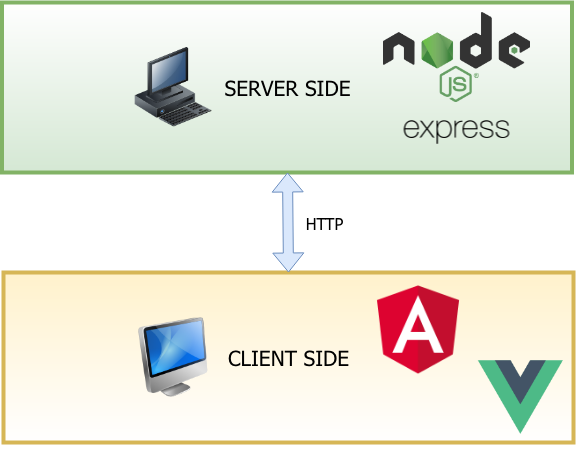
\includegraphics[scale=0.5]{images/nodejs.png}
	\caption{Ogólny schemat działania aplikacji typu klient-serwer bazującej na serwerze \textit{Node.js} oraz nowoczesnych frameworkach implementacji warstwy prezentacji}
	\label{Rys:nodejs}
\end{figure}

\section{Implementacja aplikacji serwerowej}
W poniższym rozdziale przedstawiony zostanie sposób implementacji aplikacji serwerowej bazującej na zestawie bibliotek \textit{Node.js} oraz \textit{Express.js}.

\subsection{Inicjalizacja serwera}
Inicjalizacja serwera rozpoczyna się od wygenerowania klucza i certyfikatu SSL (\textit{Secure Socket Layer}), który używany jest przez protokół HTTPS w celu zwiększenia bezpieczeństwa danych. Kolejnym krokiem jest zdefiniowanie portu, na którym będzie on nasłuchiwał żądań klienta i rozpoczęcia nasłuchiwania. W tym celu posłużono się frameworkiem \textit{Express.js} i zdefiniowano lokalny serwer HTTPS pracujący na porcie numer 9000. 

W celu wygenerowania certyfikatu i klucza RSA (\textit{Rivest-Shamir-Adleman}) posłużono się poniższą komendą:

\begin{verbatim}
openssl req -newkey rsa:2048 -new -nodes -keyout key.pem -out cert.pem
\end{verbatim}

Wygenerowany klucz RSA zawiera 2048 bitów. Rozmiar ten wybrany został z kilku powodów. Przede wszystkim wiele urządzeń nie wspiera większych wartości bitowych. Ponadto, użycie tego klucza w trakcie szyfrowania i uwierzytelniania powoduje znacznie mniejsze zużycie procesora. 

Sama, wstępna implementacja serwera HTTPS i przekazanie wygenerowanych plików \textit{key.pem} oraz \textit{cert.pem} do parametrów inicjalizacji serwera  zaprezentowana została na poniższych blokach kodu źródłowego:

\begin{verbatim}
const httpsServer = https.createServer({
key: fs.readFileSync('key.pem'),
cert: fs.readFileSync('cert.pem')
}, app);

httpServer = app.listen(9000, () => {
console.log("HTTP Server running at https://localhost:" + 
httpServer.address().port);
});
\end{verbatim}

W następnym kroku zdefiniowano komendę \textit{start-server}, za pomocą której uruchamiany będzie serwer. Definicja komendy znajduje się w pliku JSON służącym do zarządzania lokalnymi paczkami NPM (\textit{Node Package Module}) - \textit{package.json}. W celu uruchomienia serwera wystarczy użyć polecenia \textit{npm run start-server}. 

\begin{verbatim}
	"start-server": "./node_modules/.bin/ts-node ./server/server.ts --secure",
\end{verbatim}

Po uruchomieniu serwera z poziomu konsoli otrzymano komunikat widoczny na rysunku \ref{Rys:nodejs-running}.

\begin{figure}[h]
	\centering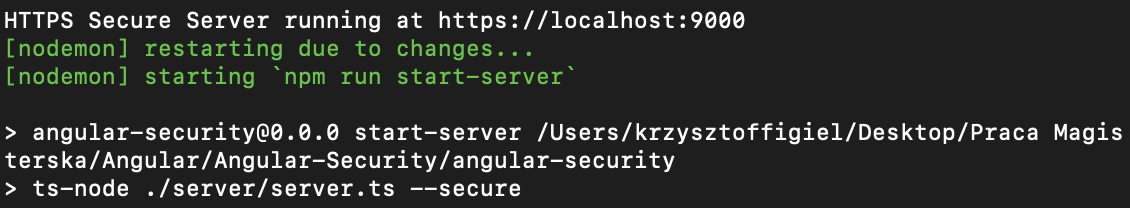
\includegraphics[scale=0.76]{images/nodejs/server-running.png}
	\caption{Zrzut ekranu konsoli systemu \textit{MacOS} ukazujący komunikaty o poprawnym uruchomieniu procesu nasłuchiwania przez serwer na porcie 9000}
	\label{Rys:nodejs-running}
\end{figure}

Definicja tabel routingu w \textit{Express.js} opiera się na użyciu funkcji \texttt{app.route(path)}. W aplikacji serwerowej zdefiniowano następujące ścieżki routingu:

\begin{itemize}
	\item \textit{/api/books}
	\item \textit{/api/signup}
	\item \textit{/api/user}
	\item \textit{/api/logout}
	\item \textit{/api/login}
\end{itemize}

Przykładowa definicja wpisu tabeli routingu zaprezentowana została na poniższym bloku kodu źródłowego:

\begin{verbatim}
app.route('/api/books')
.get(readAllBooks);
\end{verbatim}

\subsection{Implementacja modułu rejestracji nowego użytkownika} 
W następnym kroku zdefiniowano metody odpowiedzialne za obsługę rejestracji nowego użytkownika w aplikacji. Wpis tabeli routingu zawierający ścieżkę do tworzenia nowego użytkownika wygląda następująco:

\begin{verbatim}
app.route('/api/signup')
.post(createUser);
\end{verbatim}

Po zdefiniowaniu wpisu przystąpiono do implementacji metody \texttt{createUser(req, res)}. Sama implementacja tej metody opiera się na odebraniu parametrów przesyłanych przez użytkownika w obiekcie \texttt{req} i przekazania odpowiednich statusów metody HTTP do klienta (\texttt{res}) w zależności czy weryfikacja nowego użytkownika przebiegła pomyślnie czy też nie. 

Do walidacji haseł użytkownika posłużono się walidatorem z repozytorium NPM - \textit{password-validator}. Umożliwia on zdefiniowanie reguł tworzenia nowych haseł oraz dodawanie haseł, które znaleźć się mają na tzw. \textit{blacklist} czyli liście haseł niedopuszczalnych, powszechnie używanych. W celu zachowania bezpieczeństwa systemu zdefiniowano reguły i przykład \textit{blacklist} tworzenia nowych haseł przez użytkowników:

\begin{verbatim}
schema
.is().min(10)                                   // Minimum length 10
.has().uppercase()                              // Must have uppercase letters
.has().lowercase()                              // Must have lowercase letters
.has().digits()                                 // Must have digits
.has().not().spaces()                           // Should not have spaces
.is().not().oneOf(['Passw0rd', 'Password123']); // Blacklist these values
\end{verbatim}

Po pomyślnej walidacji przesyłanego przez użytkownika w obiekcie \texttt{req} hasła serwer odpowiada komunikatem 200 przesyłając w parametrze \texttt{body} dane (\textit{id} oraz \textit{email}) nowego użytkownika. W tym celu posłużono się metodą \texttt{res.status(httpCode)}:

\begin{verbatim}
res.status(200).json({ id: user.id, email: user.email });
\end{verbatim}

W przypadku podania hasła nieazgodnego z przyjętymi regułami tworzenia nowych haseł użytkownika serwer odpowiada komunikatem 400 \textit{Bad request}. Wykorzystano metodę \texttt{res.status(httpCode)}, a jako zwracany parametr podano listę błędów zwracaną przez pakiet \textit{password-validator}:

\begin{verbatim}
res.status(400).json({ errors });
\end{verbatim}

Jeżeli serwer napotkał wewnętrzny błąd, wówczas wysyła on komunikat o kodzie 500 \textit{Internal Server Error} za pomocą metody \texttt{res.sendStatus(httpCode)} bez przekazywania treści błędu w celu zachowania odpowiedniej hermetyzacji aplikacji:

\begin{verbatim}
res.sendStatus(500);
\end{verbatim}

Nowi użytkownicy przechowywani są w bazie danych za pomocą obiektu składającego się z trzech wartości:

\begin{verbatim}
const user: DbUser = {
id,
email,
passwordDigest
};
\end{verbatim}

Przy tworzeniu nowego użytkownika sprawdzany jest dodatkowo warunek czy nie ma już podobnego konta w bazie danych:

\begin{verbatim}
const usersPerEmail = _.keyBy(_.values(USERS), 'email');

if (usersPerEmail[email]) {
const message = 'User already exists with assigned email address: ' + email;
console.error(message);
throw new Error(message);
}
\end{verbatim}

Jeżeli użytkownik istnieje w bazie danych wyświetlany jest stosowny komunikat. W przypadku braku podobnego konta i pomyślnej weryfikacji tworzony i zwracany jest nowy obiekt \texttt{user}:

\begin{verbatim}
this.userCounter++;

const id = this.userCounter++;

const user: DbUser = {
id,
email,
passwordDigest
};

USERS[id] = user;

return user;
\end{verbatim}

Hasła użytkownika przechowywane są w bazie danych za pomocą funkcji skrótu \textit{Argon2}. W tym celu wykorzystano specjalny pakiet oferowany przez repozytorium NPM. Hasło podane przez użytkownika przekazywane jest jako parametr funkcji \texttt{argon2.hash(\textit{password})}. Więcej informacji na temat wykorzystania funkcji \textit{Argon2} zawarte zostało w rozdziale dotyczącym bezpieczeństwa. 

\subsection{Implementacja modułu logowania użytkownika}

\subsection{Implementacja modułu wylogowywania użytkownika}

\subsection{Implementacja mechanizmów podtrzymywania sesji użytkownika}

\chapter{Mechanizmy bezpieczeństwa aplikacji internetowych opartych na języku JavaScript}

\section{Wprowadzenie}
W poniższym rozdziale przedstawiono najważniejsze mechanizmy bezpieczeństwa wykorzystywane w aplikacjach internetowych opartych na języku \textit{JavaScript}. Działanie mechanizmów poparto przykładami pochodzącymi z aplikacji internetowej napisanej w ramach pracy magisterskiej. 

\subsection{Komunikacja klient-serwer przy użyciu protokołu HTTPS}
Protokół HTTPS (\textit{Hypertext Transfer Protocol Secure}) jest szyfrowaną wersją protokołu HTTP (\textit{Hypertext Transfer Protocol}). Komunikacja nie jest oparta bezpośrednio na modelu klient-serwer, tylko na zasadzie szyfrowanego protokołu SSL (\textit{Secure Socket Layer}). Dzięki takiemu rozwiązaniu nie ma możliwości przejęcia czy też naruszenia integralności danych przesyłanych w trakcie transmisji. SSL wykorzystuje tzw. certyfikaty mające na celu poświadczenie wiarygodności domeny, bądź domeny oraz jej właściciela. Dzięki temu użytkownik, który korzysta ze strony WWW ma pewność, że przesyłane informacje nie zostaną przechwycone i nie trafią w nieporządane ręce. W momencie nawiązywania połączenia przez przeglądarkę internetową zabezpieczoną protokołem SSL następuje ustalenie odpowiednich algorytmów oraz kluczy szyfrujących, stosowanych następnie do wymiany danych między przeglądarką a serwerem WWW. Wykorzystywana jest tutaj kryptografia asymetryczna o ustalonej długości klucza.

Inicjalizacja serwera w aplikacji rozpoczyna się od wygenerowania klucza i certyfikatu SSL. Można to wykonać za pomocą następującej komendy:

\begin{verbatim}
openssl req -newkey rsa:2048 -new -nodes -keyout key.pem -out cert.pem
\end{verbatim}

Taka komenda generuje nowy certyfikat oraz klucz prywatny RSA (o rozmiarze podanym w bitach) i zapisuje je do plików \textit{key.pem} oraz \textit{cert.pem}. W tym przypadku jest to 2048 bitowy klucz. Zawartość tych plików zostanie przekazana jako parametr metody \texttt{createServer([options], [requestListener])} pakietu NPM o nazwie \textit{https} służącej do zainicjalizowania serwera nasłuchującego na wybranym porcie. Powodem wybrania 2048 bitowego klucza był fakt, iż niektóre urządzenia nie większych wartości bitowych. Ponadto, wykorzystanie tych kluczy podczas szyfrowania i uwierzytelniania pozwala na znacznie mniejsze zużycie procesora.

\newpage
Zawartość wygenerowanych plików przedstawiono na rysunku \ref{Rys:keyandpem}.

\begin{figure}[h]
	\centering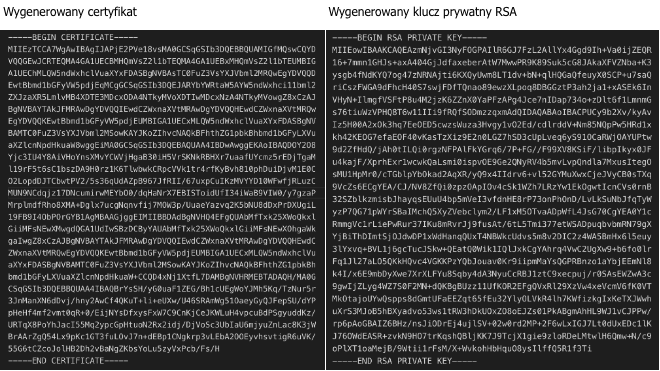
\includegraphics[scale=0.6]{images/security/key_and_certificate.png}
	\caption{Zdjęcie przedstawiające wygenerowany za pomocą komendy \textit{openssl -newkey} certyfikat SSL oraz klucz prywatny RSA.}
	\label{Rys:keyandpem}
\end{figure}

Na rysunku poniżej przedstawiono ogólny schemat działania protokołu HTTPS z wykorzystaniem protokołu SSL podczas wymiany zaszyfrowanych danych między klientem a serwerem:

\begin{figure}[h]
	\centering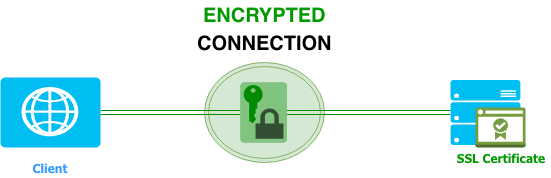
\includegraphics[scale=0.6]{images/security/how-https-works.png}
	\caption{Schemat działania protokołu HTTPS wykorzystującego protokół SSL w trakcie wymiany zaszyfrowanych danych między klientem a serwerem}
	\label{Rys:keyandpem}
\end{figure}

\subsection{Zasady tworzenia haseł użytkowników}
Hasła są obecnie jedną z najpopularniejszych technik uwierzytelniania w Internecie. Jest to metoda bardzo bezpieczna pod warunkiem spełnienia określonych kryteriów. Hasło użytkownika powinno charakteryzować się tym iż nie jest ono ciągiem składającym się z mniej niż dziesięciu znaków. Dzięki takiemu rozwiązaniu liczba możliwych kombinacji (na przykład przy ataku słownikowym) diametralnie wzrasta. Kolejną kwestią jest wykorzystywanie przez użytkowników różnych typów znaków alfanumerycznych - dużych i małych liter, znaków specjalnych oraz cyfr. Znacznie podnosi to poziom skomplikowania zabezpieczenia. 

Twórcy aplikacji internetowych mają dostęp do szeregu bibliotek i pakietów umożliwiających definiowanie reguł tworzenia bezpiecznych haseł użytkowników. W projekcie wykorzystano pakiet NPM o nazwie \textit{password-validator}. Pozwala on na proste definiowanie zasad kreowania haseł i dostarcza mechanizmy weryfikacji czy powyższe zasady zostały spełnione. 

W przykładowym projekcie posłużono się następującymi definicjami reguł:

\begin{verbatim}
schema
.is().min(10)                                   // Minimum length 10
.has().uppercase()                              // Must have uppercase letters
.has().lowercase()                              // Must have lowercase letters
.has().digits()                                 // Must have digits
.has().not().spaces()                           // Should not have spaces
.is().not().oneOf(['Passw0rd', 'Password123', '123456', '123456789', 'qwerty']); 
// Blacklist these values
\end{verbatim}
 
Jak widać, istnieje również możliwość zdefiniowania tzw. \textit{blacklisty} zawierającej najczęściej używane hasła, będące łatwym elementem do wykorzystania podczas na przykład ataku słownikowego. Do walidacji poprawności przesyłanych przez użytkownika haseł wykorzystano metodę oferowaną przez pakiet \textit{password-validator}:

\begin{verbatim}
schema.validate(password, options?)
\end{verbatim}

W przypadku wpisania przez użytkownika hasła nie spełniającego wymagań zdeklarowanych w poniższym schemacie następuje walidacja formularza rejestracji i powiadomienie użytkownika jakie błędy popełnił:

\begin{figure}[h]
	\centering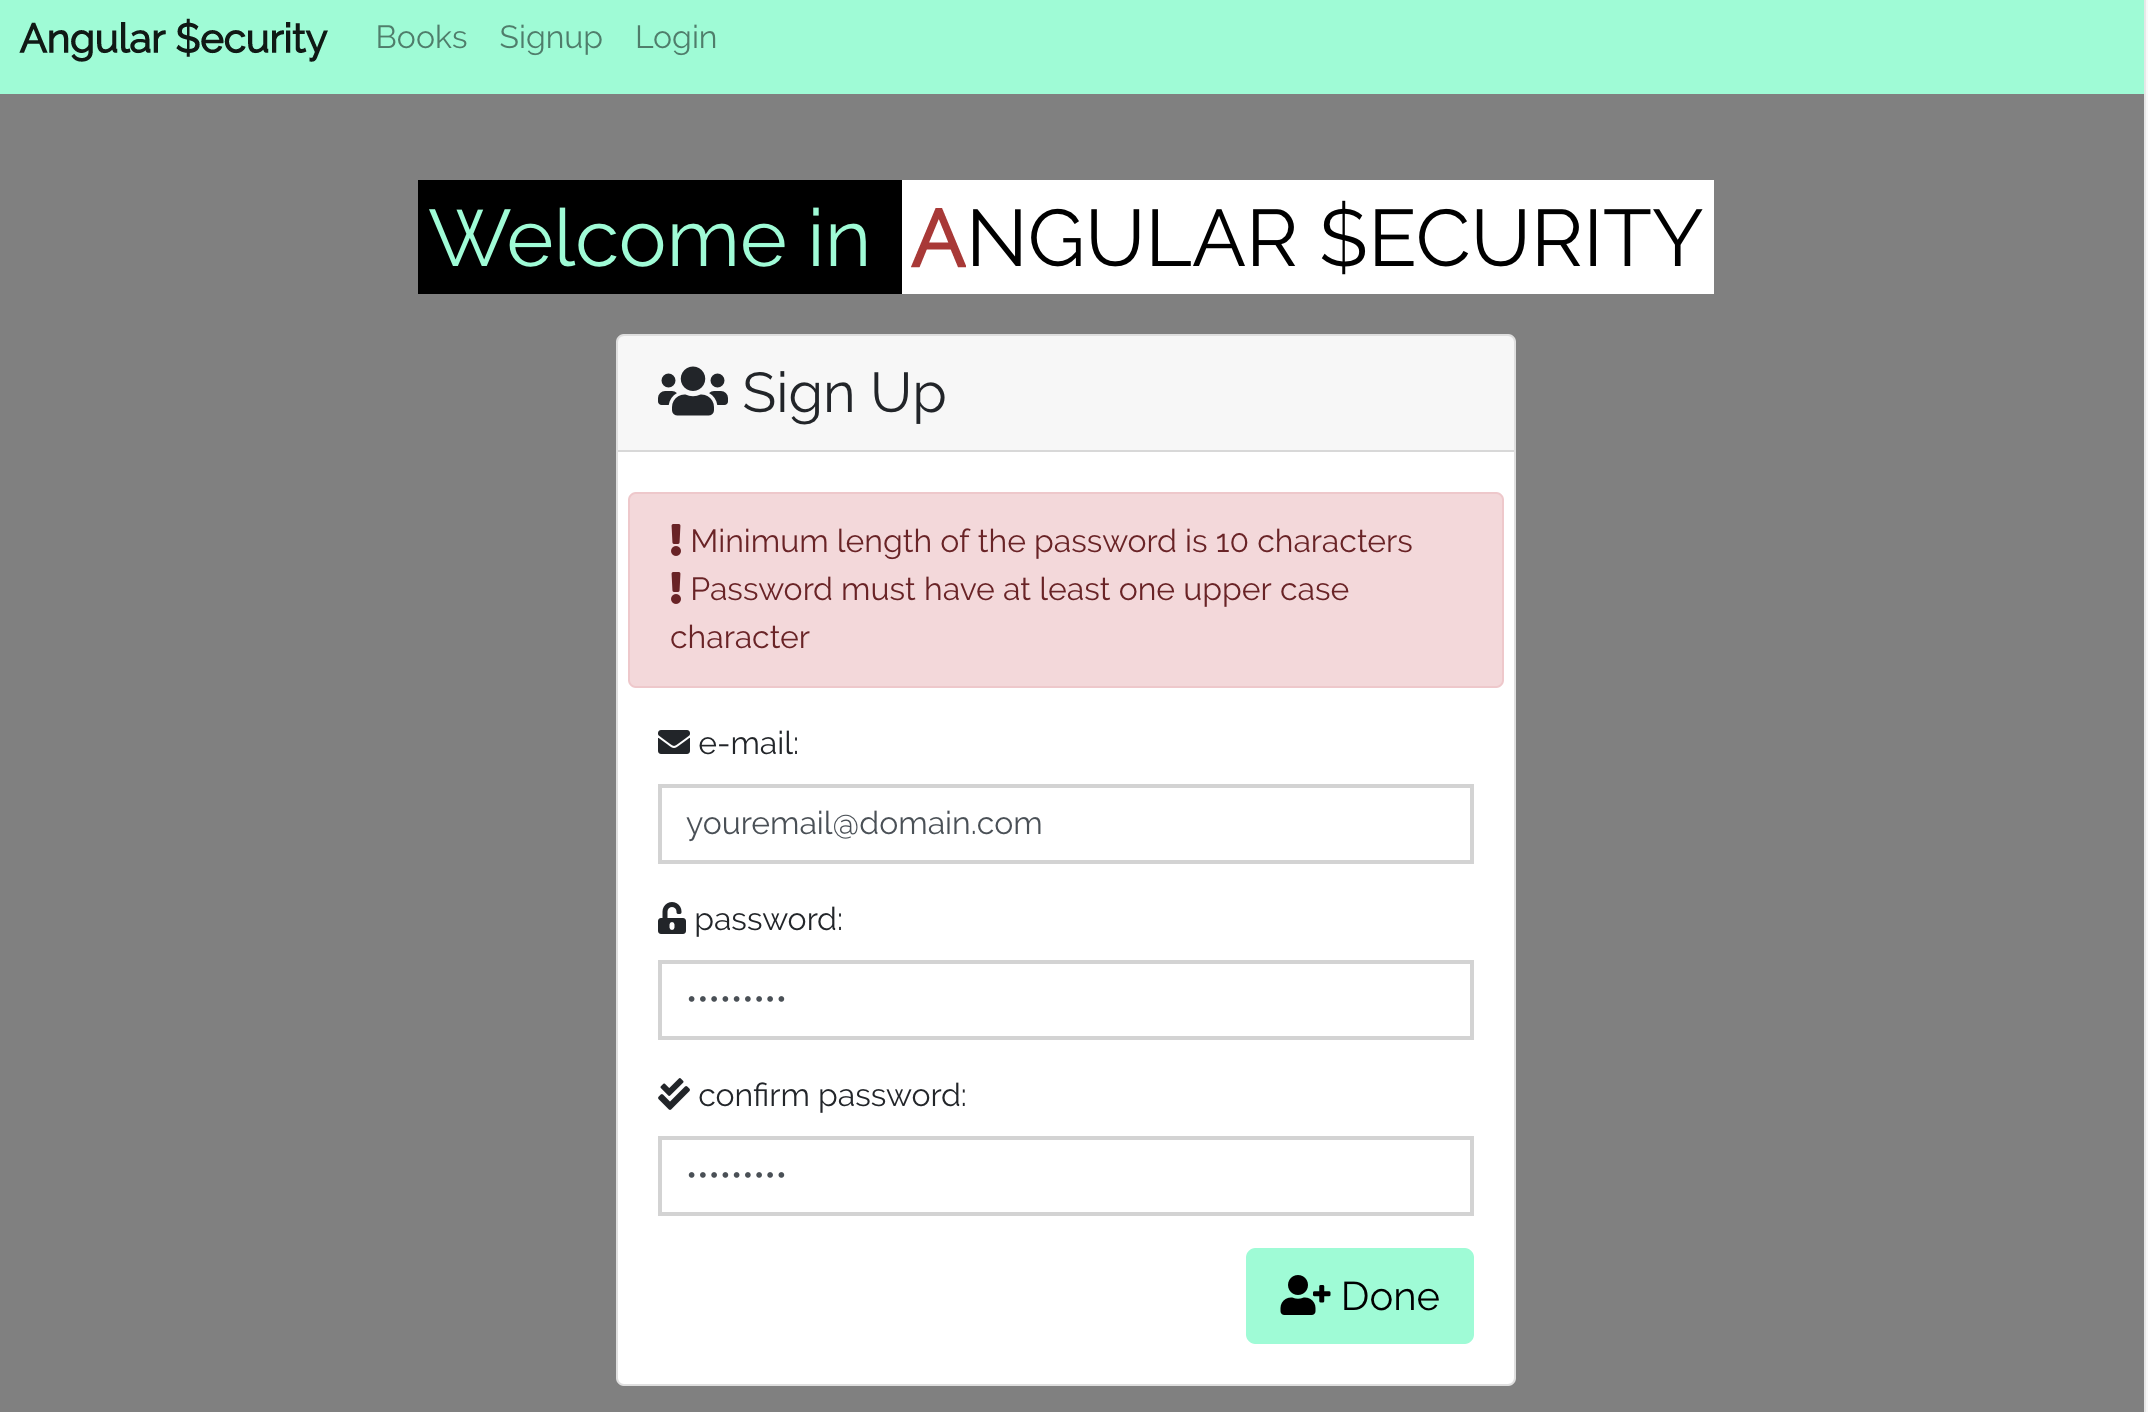
\includegraphics[scale=0.4]{images/security/password-bad-validation.png}
	\caption{Ekran aplikacji pokazowej prezentujący błędną walidację formularza w przypadku podania przez użytkownika haseł, które nie spełniają wymagań zdefiniowanych w schemacie bezpiecznego hasła.}
	\label{Rys:badpassvalid}
\end{figure}

\subsection{Sposób przechowywania haseł użytkowników}
Hasła użytkowników aplikacji przechowywane są w bazie danych w postaci jednokierunkowej funkcji skrótu \textit{Argon2}, która jest zwycięzcą konkursu \textit{Password Hashing Competition} z połowy 2015 roku. Funkcja ta jest rekomendowana przez OWASP (\textit{Open Web Application Security Project}). Jest to globalna, profesjonalna fundacja, która działa charytatywnie. OWASP jest otwarty dla każdego, kto interesuje się bezpieczeństwem nowoczesnych aplikacji internetowych. Organizacja działa na rzecz publikowania artykułów, metodologii, narzędzi i dokumentacji związanych z ochroną danych. 

Funkcja \textit{Argon2} może być używana do mieszania haseł, przechowywania danych uwierzytelniających, pochodnych kluczy lub innych aplikacji. W przeciwieństwie do funkcji \textit{bcrypt} czy \textit{PBKDF2}, \textit{Argon2} cechuje się wysoką adaptacyjnością. Możliwe jest tu bowiem ustawienie aż trzech parametrów: liczby iteracji wykonywanych operacji kryptograficznych, wielkości wykorzystywanej pamięci oraz zrównoleglenia, czyli liczby równoległych wątków działających w tle. Ma ona bardzo prostą konstrukcję umożliwiającą mniejsze zużycie pamięci i efektywne wykorzystanie wielu jednostek obliczeniowych w celu przeprowadzania działań kryptograficznych. Jedną z ciekawych funkcji jest również możliwość sprecyzowania dodawanej soli, długości wyjściowego skrótu czy też możliwość dodania dodatkowego, opcjonalnego klucza. \textit{Argon2} posiada trzy odmiany: \textit{Argon2i}, \textit{Argon2d} oraz \textit{Argon2id}. Funkcja \textit{Argon2d} jest znacznie szybsza od pozostałych i jednocześnie odporna na ataki typu \textit{GPU Cracking}. \textit{Argon2i} charakteryzuje się znacznie większą liczbą odwołań do pamięci co powoduje ją wolniejszą od pozostałych. Zaleca się używanie jej do hashowania haseł. Ostatnia z odmian - \textit{Argon2id} - jest hybrydą dwóch wersji: \textit{Argon2i} oraz \textit{Argon2d}. Czyni ją to odporną na ataki typu \textit{side-channel} i zwiększa jej bezpieczeństwo na metody naruszania zabezpieczeń z użyciem kart graficznych. Ogólna, bardzo uproszczona postać funkcji \textit{Argon2} wygląda następująco:

\begin{verbatim}
ARGON2(password, salt, parallelism, length, memory, count, key)
\end{verbatim}

Jak widać, oprócz przekazania takich parametrów jak hasło czy dodawana sól istnieje równiez możliwość oznaczenia poziomu zrównoleglenia obliczeń (\texttt{parallelism}), określenia ilości pamięci niezbędnej do obliczenia skrótu (\texttt{memory}), określenia opcjonalnego klucza (\texttt{key}) czy też wielkości ciągu wyjściowego (\texttt{count}). Cały algorytm oparty jest o kryptograficzną funkcję skrótu \textit{BLAKE2}, która jest jednym z finalistów konkursu \textit{SHA-3}. 

W autorskiej aplikacji wykorzystano pakiet NPM o nazwie \textit{node-argon2}. Oferuje on większość możliwości, które dostarcza funkcja \textit{argon2}. Funkcja hashowania hasła użytkownika wygląda następująco:

\begin{verbatim}
async function createUserAndSession(res: Response, credentials) {
const passwordDigest = await argon2.hash(credentials.password);
...
}
\end{verbatim}

Jak widać jako parametr funkcji przekazywane jest hasło podane przez użytkownika w trackie rejestracji do serwisu. Rezultat hashowania hasła widoczny jest na zdjęciu \ref{Rys:argon2}.

\begin{figure}[h]
	\centering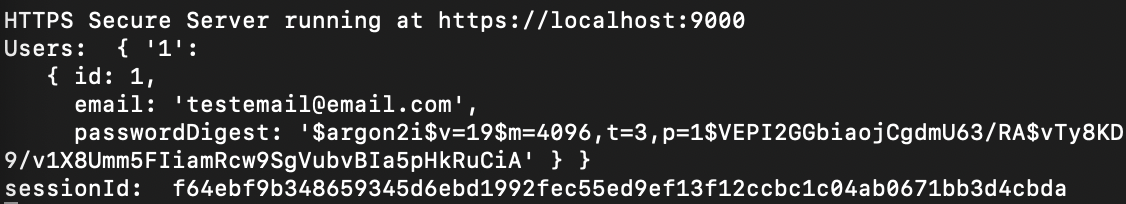
\includegraphics[scale=0.75]{images/security/argon2.png}
	\caption{Okno konsoli serwera po pomyślnej rejestracji nowego użytkownika z wyświetlonym skrótem hasła podanego przez osobę rejestrującą się do serwisu..}
	\label{Rys:argon2}
\end{figure}

Funkcja \texttt{argon2.hash(password, {options})} umożliwia określenie rodzaju funkcji \textit{argon2}. Wystarczy w obiekcie options przekazać wartość \texttt{type: typeOfArgonFunction}. Przykładowy rezultat hashowania hasła \textit{PAssw0rd12} oraz kod źródłowy przedstawione zostały poniżej:

\begin{verbatim}
argon2.hash(password, {type: argon2.argon2id}).then(hash => {
console.log('Argon2id password: ', hash);
}, (err) => {
console.err('An error occured while password hashing: ', err);
});
\end{verbatim}

\begin{figure}[h]
	\centering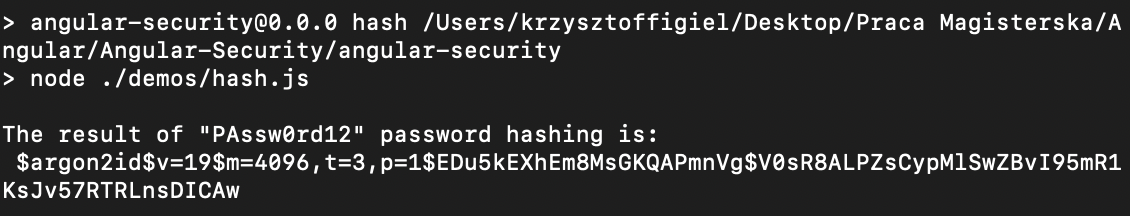
\includegraphics[scale=0.73]{images/security/argon2id.png}
	\caption{Rezultat hashowania hasła \textit{PAssw0rd12} za pomocą funkcji skrótu \textit{Argon2id}.}
	\label{Rys:argon2id}
\end{figure}

Pakiet \textit{node-argon2} oferuje również możliwość weryfikowania hasła. Służy do tego metoda \texttt{argon2.verify('<big long hash>', 'password')}. Rezultat weryfikacji hasła \textit{PAssw0rd12} widoczny jest na zdjęciu \ref{Rys:argon2idmatchfailed}.

\begin{figure}[h]
	\centering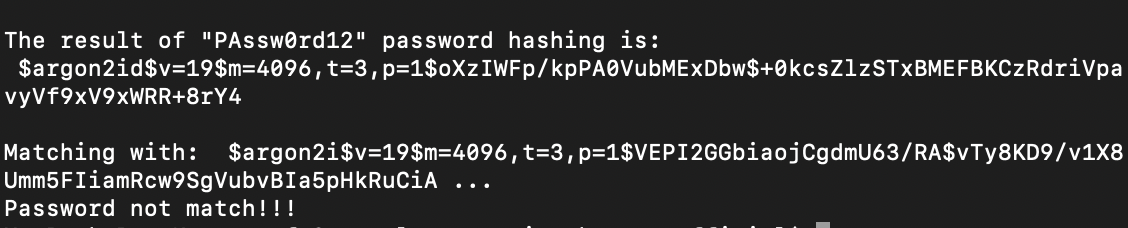
\includegraphics[scale=0.73]{images/security/argon-matching-failed.png}
	\caption{Rezultat wykorzystania funkcji sprawdzającej błędne dopasowanie hasła do funkcji skrótu stworzonego za pomocą \textit{Argon2id}.}
	\label{Rys:argon2idmatchfailed}
\end{figure}

W momencie podstawienia innego skrótu (w tym przypadku skrótu wygenerowanego przez funkcję \textit{argon2i}) metoda program informuje użytkownika o błędnym dopasowaniu hasła. 

\subsection{Mechanizmy podtrzymywania sesji użytkownika}

\subsection{JSON Web Tokens}

\subsection{Metody ochrony aplikacji internetowych przed atakami typu CSRF}

\subsection{Metody ochrony aplikacji internetowych przed atakami typu XSS}


\subsection{Metody ochrony aplikacji internetowych przed atakami typu CSS}

\subsection{Walidacja formularzy}

\subsection{Autoryzacja oparta na rolach użytkowników (RBAC)}

\subsection{Testy aplikacji internetowych z użyciem frameworków Jasmine oraz Karma}



\chapter{Baza danych}

\section{Opis tabeli bazy danych}
W poniższej sekcji opisane zostaną tabele bazy danych wraz z polami w nich zawartymi. Określony zostanie typ danego pola oraz krótki opis jego przeznaczenia. 

\subsection{Person}
Tabela \textit{person} -- zawiera dane dotyczące użytkownika aplikacji:
\begin{itemize}
	\item \textit{id} -- pole typu \textit{INT} zawierające unikalny identyfikator pola w bazie danych,
	\item \textit{name} -- pole typu \textit{VARCHAR} przechowujące imię użytkownika,
	\item \textit{surname} -- pole typu \textit{VARCHAR}  przechowujące nazwisko użytkownika,
	\item \textit{pesel} -- pole typu \textit{VARCHAR} przechowujące PESEL użytkownika,
	\item \textit{guardian} -- pole typu \textit{VARCHAR} mówiące o tym, czy dany użytkownik posiada opiekuna,
	\item \textit{street} -- pole typu \textit{VARCHAR} przechowujące nazwę ulicy, na której mieszka użytkownik,
	\item \textit{homeNumber} -- pole typu \textit{VARCHAR} przechowujące numer domu, pod którym mieszka użytkownik,
	\item \textit{city} -- pole typu \textit{VARCHAR} przechowujące nazwę miasta, w którym mieszka użytkownik,
	\item \textit{postalCode} -- pole typu \textit{VARCHAR} przechowujące kod pocztowy miasta, w którym mieszka użytkownik,
	\item \textit{telephoneNumber} -- pole typu \textit{VARCHAR} przechowujące numer telefonu użytkownika,
	\item \textit{actualGlucometer} -- pole typu \textit{INT} będące kluczem obcym z tabeli \textit{glucometer}, zawierające \textit{id} aktualnie posiadanego glukometru,
	\item \textit{previousGlucometer} -- pole typu \textit{INT} będące kluczem obcym z tabeli \textit{glucometer}, zawierające \textit{id} poprzedniego glukometru,
	\item \textit{serialNumber} -- pole typu \textit{VARCHAR} przechowujące numer seryjny glukometru, którego aktualnie używa użytkownik.
\end{itemize}

\subsection{Medical Data}
Tabela \textit{medical\_data} -- zawiera informacje dotyczące danych medycznych użytkownika:
\begin{itemize}
	\item \textit{id} -- pole typu \textit{INT} zawierające unikalny identyfikator pola w bazie danych,
	\item \textit{yearOfIllness} -- pole typu \textit{TEXT} przechowujące informację na temat roku zachorowania użytkownika na cukrzycę,
	\item \textit{otherMedicines} -- pole typu \textit{VARCHAR}  przechowujące informacje na temat innych, przyjmowanych leków,
	\item \textit{bmi} -- pole typu \textit{DECIMAL} przechowujące wartość współczynnika BMI \textit{(Body Mass Index)} użytkownika,
	\item \textit{height} -- pole typu \textit{INT} przechowujące informacje na temat wzrostu użytkownika w~ cm,
	\item \textit{weight} -- pole typu \textit{VARCHAR} przechowujące informacje na temat wagi użytkownika,
	\item \textit{hbValue} -- pole typu \textit{DECIMAL} przechowujące informacje na temat wartości współczynnika HbA1c użytkownika,
	\item \textit{diabetesTypeId} -- pole typu \textit{INT} będące kluczem obcym z tabeli \textit{diabetes\_type}, zawierające \textit{id} typu cukrzycy, na którą cierpi użytkownik,
	\item \textit{insulinId} -- pole typu \textit{INT} będące kluczem obcym z tabeli \textit{insulin}, zawierające \textit{id} typu insuliny, którą zażywa użytkownik,
	\item \textit{tabetsId} -- pole typu \textit{INT} będące kluczem obcym z tabeli \textit{tablets}, zawierające \textit{id} leku, który przyjmuje użytkownik.
\end{itemize}

\subsection{Glucometer}
Tabela \textit{glucometer} -- zawiera informacje dotyczące dostępnych glukometrów w bazie danych:
\begin{itemize}
	\item \textit{id} -- pole typu \textit{INT} zawierające unikalny identyfikator pola w bazie danych,
	\item \textit{glucometerName} -- pole typu \textit{VARCHAR} zawierające nazwę danego glukometru.
\end{itemize}

\subsection{Medical Data has Tablets}
Tabela \textit{medical\_data\_has\_tablets} -- zawiera informacje dotyczące przyjmowanych przez danego użytkownika leków:
\begin{itemize}
	\item \textit{id} -- pole typu \textit{INT} zawierające unikalny identyfikator pola w bazie danych,
	\item \textit{medicalDataId} -- pole typu \textit{INT} będące kluczem obcym z tabeli \textit{medical\_data}, zawierające \textit{id} danych medycznych danego użytkownika,
	\item \textit{tabetsId} -- pole typu \textit{INT} będące kluczem obcym z tabeli \textit{tablets}, zawierające \textit{id} leku, który przyjmuje użytkownik.
\end{itemize}

\subsection{Tablets}
Tabela \textit{tablets} -- zawiera informacje dotyczące dostępnych leków w bazie danych:
\begin{itemize}
	\item \textit{id} -- pole typu \textit{INT} zawierające unikalny identyfikator pola w bazie danych,
	\item \textit{datbletName} -- pole typu \textit{VARCHAR} zawierające nazwę danego medykamentu.
\end{itemize}

\subsection{Medical Data has Insulin}
Tabela \textit{medical\_data\_hasinsulin} -- zawiera informacje dotyczące insuliny przyjmowanej przez danego użytkownika:
\begin{itemize}
	\item \textit{id} -- pole typu \textit{INT} zawierające unikalny identyfikator pola w bazie danych,
	\item \textit{medicalDataId} -- pole typu \textit{INT} będące kluczem obcym z tabeli \textit{medical\_data}, zawierające \textit{id} danych medycznych danego użytkownika,
	\item \textit{insulinId} -- pole typu \textit{INT} będące kluczem obcym z tabeli \textit{insulin}, zawierające \textit{id} typu insuliny, którą zażywa użytkownik.
\end{itemize}

\subsection{Diabetes Type}
Tabela \textit{diabetes\_type} -- zawiera informacje dostępnych w bazie danych typów cukrzycy:
\begin{itemize}
	\item \textit{id} -- pole typu \textit{INT} zawierające unikalny identyfikator pola w bazie danych,
	\item \textit{typeName} -- pole typu \textit{VARCHAR} zawierające nazwę danego typu cukrzycy.
\end{itemize}

\subsection{Insulin}
Tabela \textit{insulin} -- zawiera informacje dotyczące dostępnych w bazie danych rodzajów insuliny:
\begin{itemize}
	\item \textit{id} -- pole typu \textit{INT} zawierające unikalny identyfikator pola w bazie danych,
	\item \textit{insulinName} -- pole typu \textit{VARCHAR} zawierające nazwę danego typu insuliny.
\end{itemize}

\subsection{Measurement}
Tabela \textit{measurement} -- zawiera informacje dotyczące pomiarów dokonywanych przez użytkowników:
\begin{itemize}
	\item \textit{id} -- pole typu \textit{INT} zawierające unikalny identyfikator pola w bazie danych,
	\item \textit{date} -- pole typu \textit{DATETIME} zawierające datę aktualnie dokonanego przez użytkownika pomiaru,
	\item \textit{glicemy} -- pole typu \textit{INT} zawierające wartość glikemii, którą wprowadza użytkownik,
	\item \textit{moment} -- pole typu \textit{TEXT} zawierające informację na temat momentu dokonanego pomiaru,
	\item \textit{note} -- pole typu \textit{VARCHAR} zawierające notatkę dotyczącą pomiaru dokonanego przez użytkownika.
\end{itemize}

\subsection{Measurement has Insulin}
Tabela \textit{measure\_has\_person} -- grupuje informacje dotyczące danego pomiaru, wykonanego przez daną osobę: 
\begin{itemize}
	\item \textit{id} -- pole typu \textit{INT} zawierające unikalny identyfikator pola w bazie danych,
	\item \textit{measurementId} -- pole typu \textit{INT} będące kluczem obcym z tabeli \textit{measurement}, zawierające \textit{id} pomiaru dokonanego przez użytkownika,
	\item \textit{personId} -- pole typu \textit{INT} będące kluczem obcym z tabeli \textit{person}, zawierające \textit{id} osoby, dokonującej pomiaru.
\end{itemize}

\subsection{Glycemia Ranges}
Tabela \textit{glycemia\_ranges} -- zawiera informacje dotyczące zakresów glikemii użytkownika:
\begin{itemize}
	\item \textit{id} -- pole typu \textit{INT} zawierające unikalny identyfikator pola w bazie danych,
	\item \textit{hipoglicemy} -- pole typu \textit{INT} zawierające wartość hipoglikemii użytkownika,
	\item \textit{hiperglicemy} -- pole typu \textit{INT} zawierające wartość hiperglikemii mierzonej przez użytkownika,
	\item \textit{hiperglicemyMeal} -- pole typu \textit{INT} zawierające wartość hiperglikemii, mierzonej przez użytkownika po posiłku.
\end{itemize}

\subsection{Products}
Tabela \textit{products} -- zawiera informacje dotyczące dostępnych w bazie danych produktów:
\begin{itemize}
	\item \textit{id} -- pole typu \textit{INT} zawierające unikalny identyfikator pola w bazie danych,
	\item \textit{productName} -- pole typu \textit{VARCHAR} przechowujące nazwę danego produktu,
	\item \textit{kcal} -- pole typu \textit{INT} zawierające ilość kalorii, które zawiera dany produkt,
	\item \textit{protein} -- pole typu \textit{DECIMAL} zawierające ilość białka, które zawiera dany produkt,
	\item \textit{fat} -- pole typu \textit{DECIMAL} zawierające ilość tłuszczu, który zawiera dany produkt,
	\item \textit{carbohydrates} -- pole typu \textit{DECIMAL} zawierające ilość węglowodanów, które zawiera dany produkt,
	\item \textit{fiber} -- pole typu \textit{DECIMAL} zawierające ilość błonnika, który zawiera dany produkt,
	\item \textit{portion} -- pole typu \textit{DECIMAL} zawierające wielkość porcji danego produktu.
\end{itemize}

\section{Model bazy danych}

Rysunek \ref{Rys:diagram-eer} przedstawia schemat EER (\textit{Enhanced Entity–Relationship}) modelu bazy danych użytego do gromadzenia informacji w systemie. Dla każdej tabeli został określony klucz główny, który może być używany w innych tabelach jako klucz obcy. Każde z pól w~ bazie danych zawiera określony typ, w zależności od tego jakie informacje ma dane pole zawierać. Tabele zawarte w bazie połączone są między sobą relacjami:
\begin{itemize}
	\item jeden-do-jeden,
	\item jeden-do-wielu,
	\item wiele-do-wielu.
\end{itemize}
W przypadku relacji wiele-do-wielu wykorzystana została tabela grupująca klucze obce z~ obydwu łączonych w tę relację tabel. 

Schemat EER bazy danych został wygenerowany automatycznie za pomocą programu \textit{MySQL Workbench} w wersji 6.3 za pomocą narzędzia \textit{Reverse Engineer}.

\begin{figure}[t]
	\centering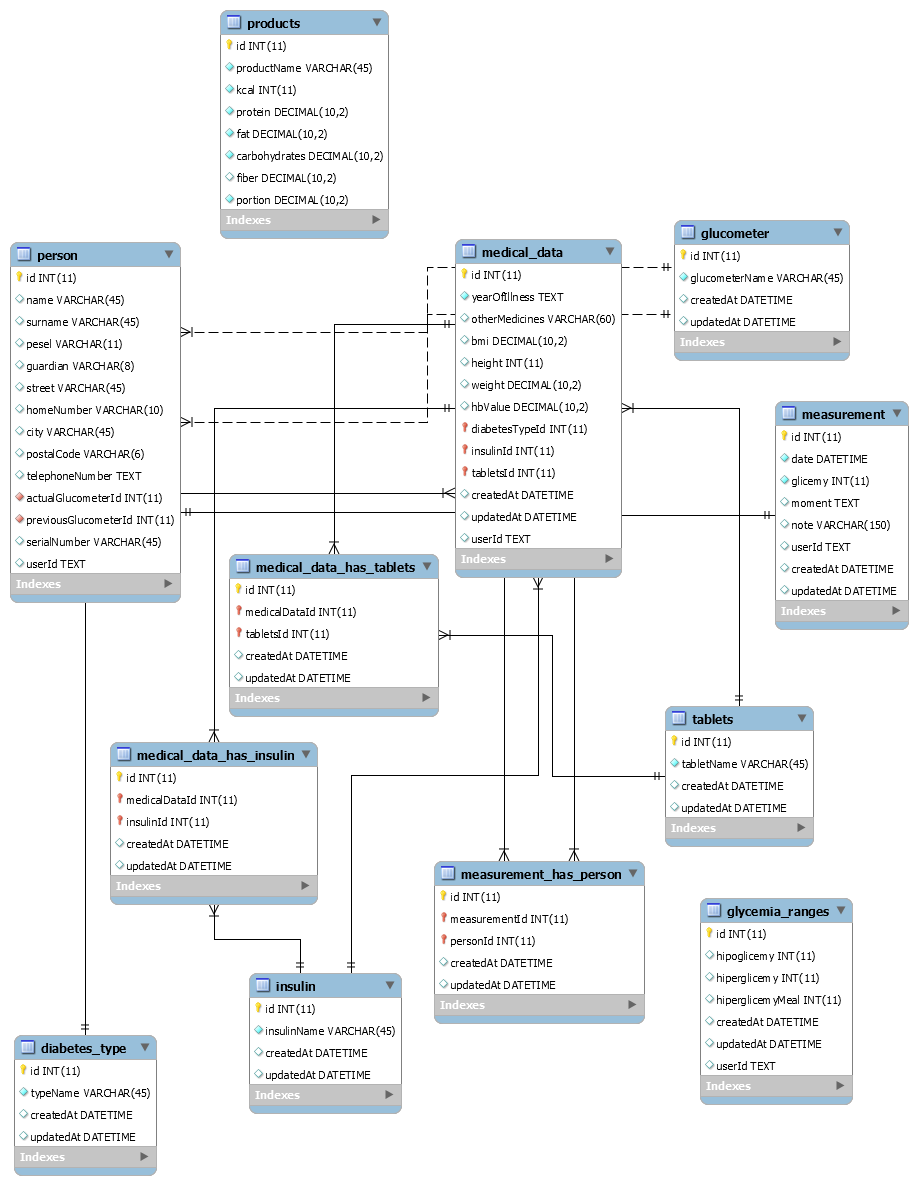
\includegraphics[scale=0.5]{images/dialog_eer.png}
	\caption{Diagram EER bazy danych aplikacji}
	\label{Rys:diagram-eer}
\end{figure}

Zapytania do bazy danych generowane są w sposób automatyczny za pomocą ORM \textit{Sequelize} na podstawie odwzorowanego w kodzie źródłowym modelu bazy danych. Cała baza danych w~ programie została wygenerowana w konwecji \textit{Code First} -- najpierw stworzony był model, a następnie na podstawie tego modelu odpowiadająca mu tabela bazy danych. Poniższy kod przedstawia przykładową implementację modelu tabeli \textit{products}:

\begin{verbatim}
module.exports = function(sequelize, DataTypes) {
	return sequelize.define('products', {
	id: {
	type: DataTypes.INTEGER(11),
	allowNull: false,
	primaryKey: true,
	autoIncrement: true
	},
	productName: {
	type: DataTypes.STRING(45),
	allowNull: false
	},
	kcal: {
	type: DataTypes.INTEGER(11),
	allowNull: false
	},
	protein: {
	type: DataTypes.DECIMAL,
	allowNull: false
	},
	fat: {
	type: DataTypes.DECIMAL,
	allowNull: false
	},
	carbohydrates: {
	type: DataTypes.DECIMAL,
	allowNull: false
	},
	fiber: {
	type: DataTypes.DECIMAL,
	allowNull: true
	},
	portion: {
	type: DataTypes.DECIMAL,
	allowNull: false
	}
	}, {
	tableName: 'products',
	timestamps : false
	});
	};
}
\end{verbatim}

Początkowo eksportowany jest model przy użyciu funkcji ORM \textit{Sequelize}. Zwracana wartość zawiera odwzorowanie tabeli produkt, na podstawie którego generowane są później automatyczne zapytania do bazy danych. Każde pole tabeli opisywane jest w następujący sposób:

\begin{verbatim}
nazwa_pola: {
	type: typ_pola,
	...
	//odpowiednie opcje i ograniczenia
}
\end{verbatim}

Ograniczenia jakie zostały użyte do zdefiniowania klucza głównego to:

	\begin{verbatim}
	allowNull: false;
	primaryKey: true;
	autoIncrement: true;
	\end{verbatim}

Pierwsze z nich określa czy pole tabeli może być wartością pustą (\textit{NULL}). Klucz główny nie może być wartością pustą, dlatego wartość ta jest ustawiona na \textit{false}. Następna wartość określa czy dane pole jest kluczem głównym. W tym przypadku przyjmuje ono wartość \textit{true}. Ostatnim z~ pól jest określenie autoinkrementowania wartości \textit{id}, dlatego również przyjmuje ono wartość \textit{true}. Ostatni znacznik:

	\begin{verbatim}
	timestamps: false
	\end{verbatim}
określa anulowanie możliwości korzystania z automatycznych znaczników czasu tworzonych w momencie edycji \textit{UPDATE} tabeli.

\chapter{Panel administratora}

\section{Logowanie do panelu administratora}
W poniższej sekcji przedstawiony zostanie proces logowania do panelu administratora w aplikacji. W pierwszej kolejności użytkownik musi wybrać opcję \textit{Rozpocznij}, dostępną z~ poziomu górnego menu na stronie głównej, a następnie wybrać przycisk \textit{Logowanie z~ Google}. Poniższy rysunek \ref{Rys:logowanieee} przedstawia okno logowania administratora.

\begin{figure}[h]
	\centering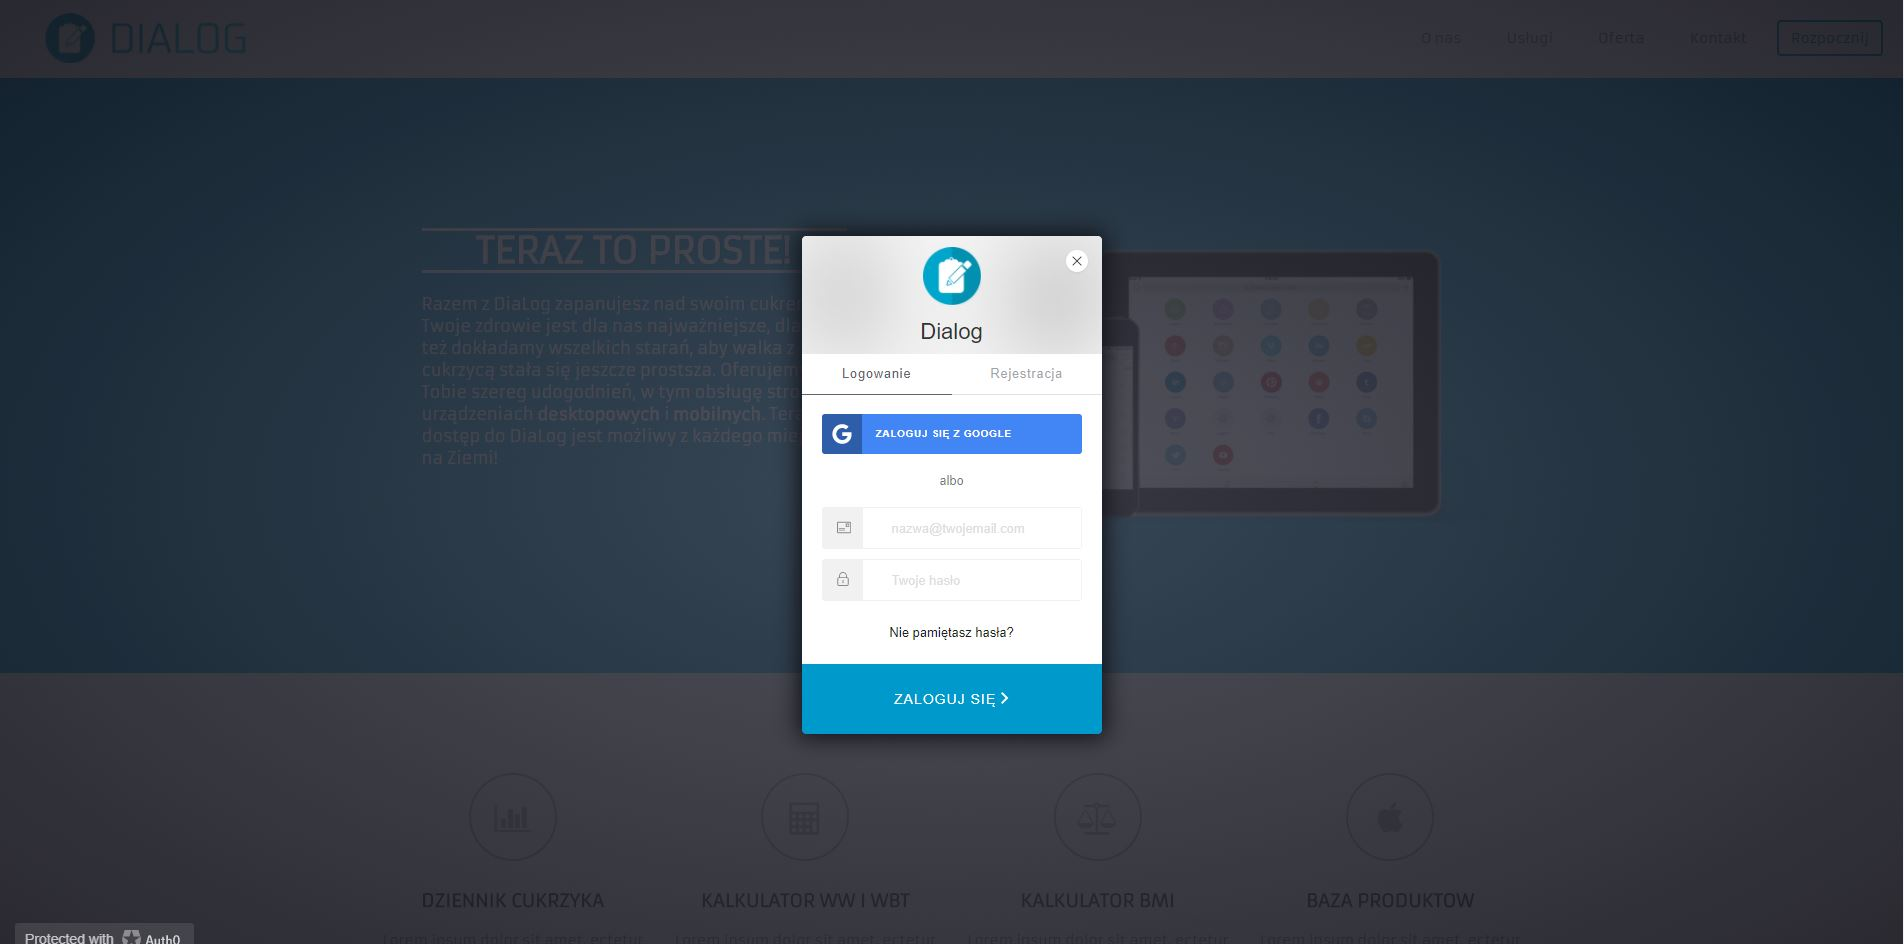
\includegraphics[scale=0.3]{images/logowanie_google.jpg}
	\caption{Okno logowania administratora}
	\label{Rys:logowanieee}
\end{figure}

Po wybraniu przycisku \textit{Logowanie z Google} należy zalogować się na konto z przypisanymi uprawnieniami administracyjnymi. Pojawi się wówczas dodatkowa pozycja w menu górnym -- \textit{Admin}, co przedstawione zostało na rysunku \ref{Rys:ekran_admin}.

\newpage

\begin{figure}[h]
	\centering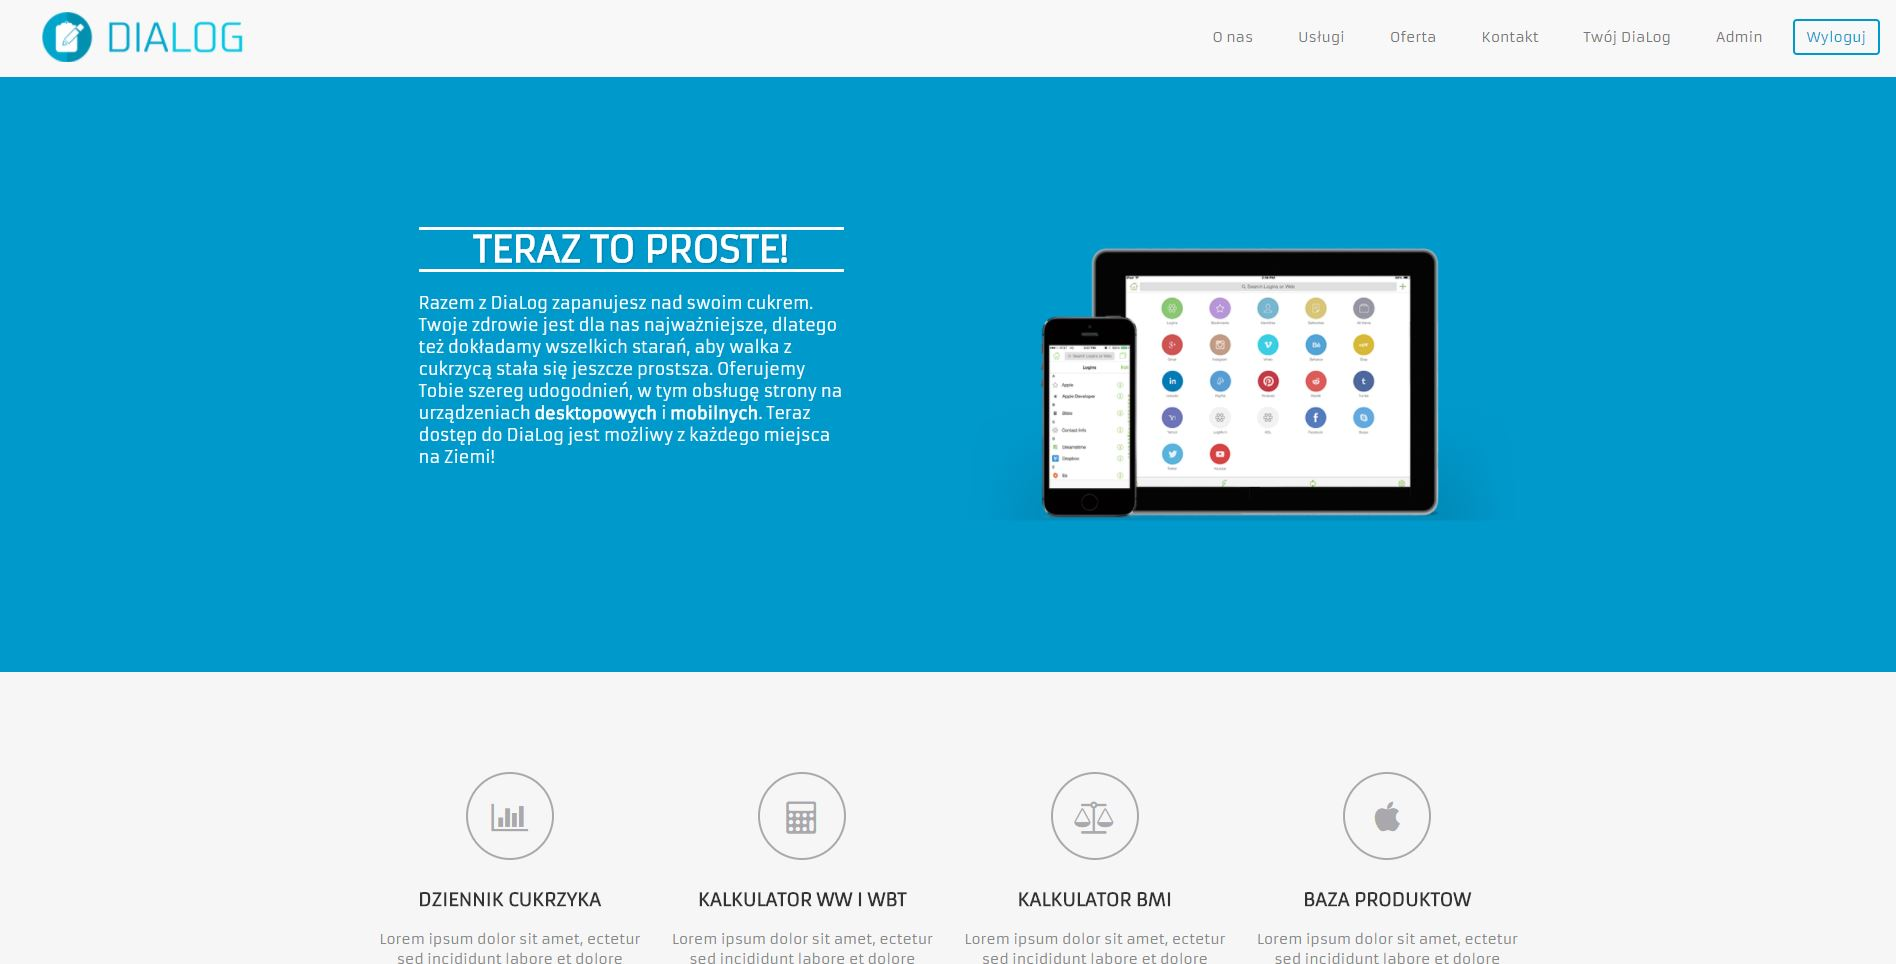
\includegraphics[scale=0.3]{images/ekran_admin.jpg}
	\caption{Okno główne aplikacji z dostępną opcją panelu administratora}
	\label{Rys:ekran_admin}
\end{figure}

\section{Użytkowanie panelu administratora}
Po kliknięciu przycisku \textit{Admin} użytkownik uzyskuje dostęp do Panelu Administratora. Panel ten został stworzony wyłącznie po to, aby usuwać błędnie dodane, bądź zduplikowane produkty dodane do bazy danych produktów. Jest to niezbędny element w przypadku funkcjonalności danej aplikacji rozszerzanych przez użytkowników. Dzięki takiemu rozwiązaniu Administrator w prosty sposób może kontrolować treść zawartą na stronie i~ w razie potrzeby usuwać ją. Panel administratora przedstawiony został na rysunku   \ref{Rys:panel_admin}. Panel został zaprojektowany w postaci tabeli tak, aby w prosty i przejrzysty sposób zaprezentować wszystkie dostępne dane. Ponieważ baza produktów może być stale rozszerzana, a ich ilość może sięgać nawet kilkuset elementów, zastosowana została paginacja tabeli, dzieląca jej zawartość na strony zawierające po dziesięć elementów.


\begin{figure}[h]
	\centering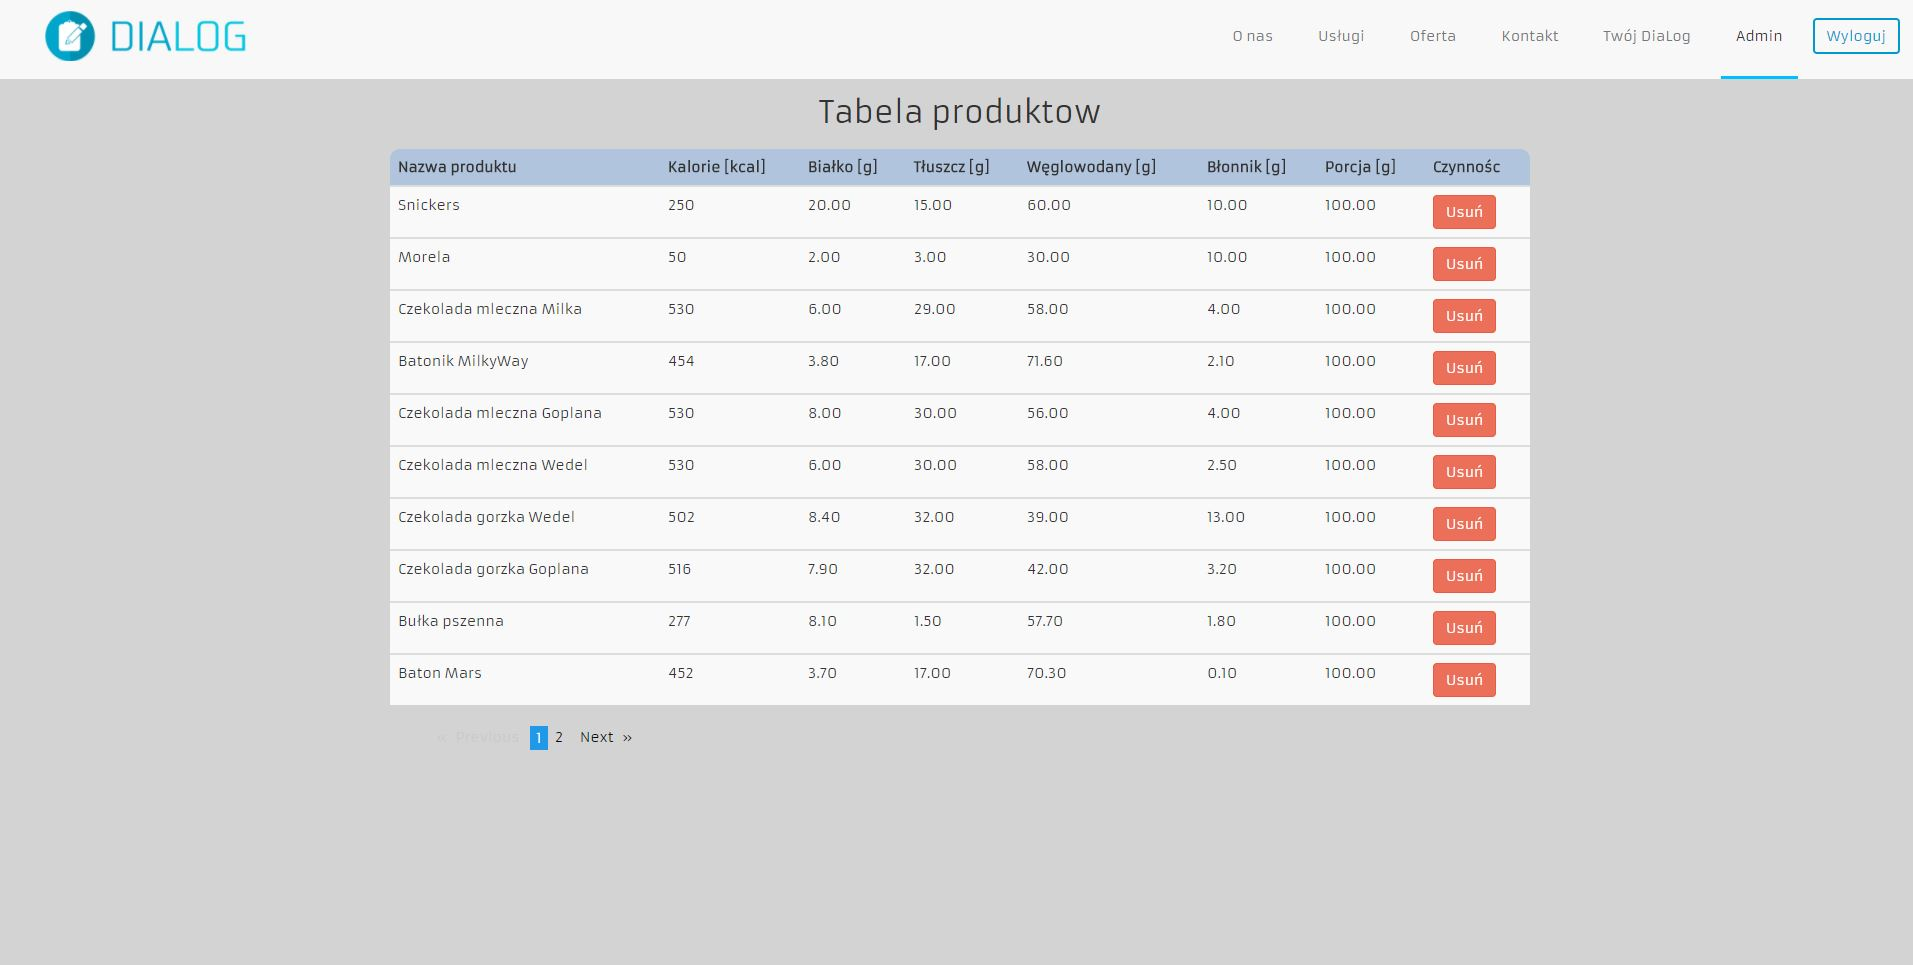
\includegraphics[scale=0.3]{images/panel_admin.jpg}
	\caption{Panel administratora aplikacji}
	\label{Rys:panel_admin}
\end{figure}

Tabela podzielona jest na osiem kolumn:
\begin{enumerate}
	\item \textit{Nazwa produktu},
	\item \textit{Kalorie [kcal]},
	\item \textit{Białko [g]},
	\item \textit{Tłuszcz [g]},
	\item \textit{Węglowodany [g]},
	\item \textit{Błonnik [g]},
	\item \textit{Porcja [g]},
	\item \textit{Czynność}.
\end{enumerate}

W kolumnie \textit{Czynność} przy każdym z wierszy dostępny jest przycisk \textit{Usuń}, dzięki któremu Administrator może usunąć wybrany produkt. Usuwanie produktu odbywa się w~ sposób dynamiczny, co oznacza, że produkt po usunięciu od razu (bez odświeżenia strony) znika z listy dostępnych produktów i nie jest on dostępny nawet z poziomu tabeli produktów dostępnej w zakładce \textit{Kalkulatory} z poziomu panelu użytkownika zalogowanego. 

Administrator, tak jak każdy zalogowany użytkownik, ma również możliwość korzystania ze wszystkich funkcjonalności systemu przeznaczonych dla tej grupy użytkowników -- zakładka \textit{Twój DiaLog}.


\chapter{Panel użytkownika zarejestrowanego}

\section{Logowanie do panelu użytkownika}
W poniższej sekcji przedstawiony zostanie proces logowania do panelu użytkownika w~ aplikacji. W pierwszej kolejności użytkownik musi wybrać opcję \textit{Rozpocznij}, dostępną z~ poziomu górnego menu na stronie głównej, a następnie wpisać login i hasło, bądź wybrać przycisk \textit{Zaloguj się z~ Google}. Okno logowania przedstawione jest na rysunku \ref{Rys:logowanie}.

\begin{figure}[h]
	\centering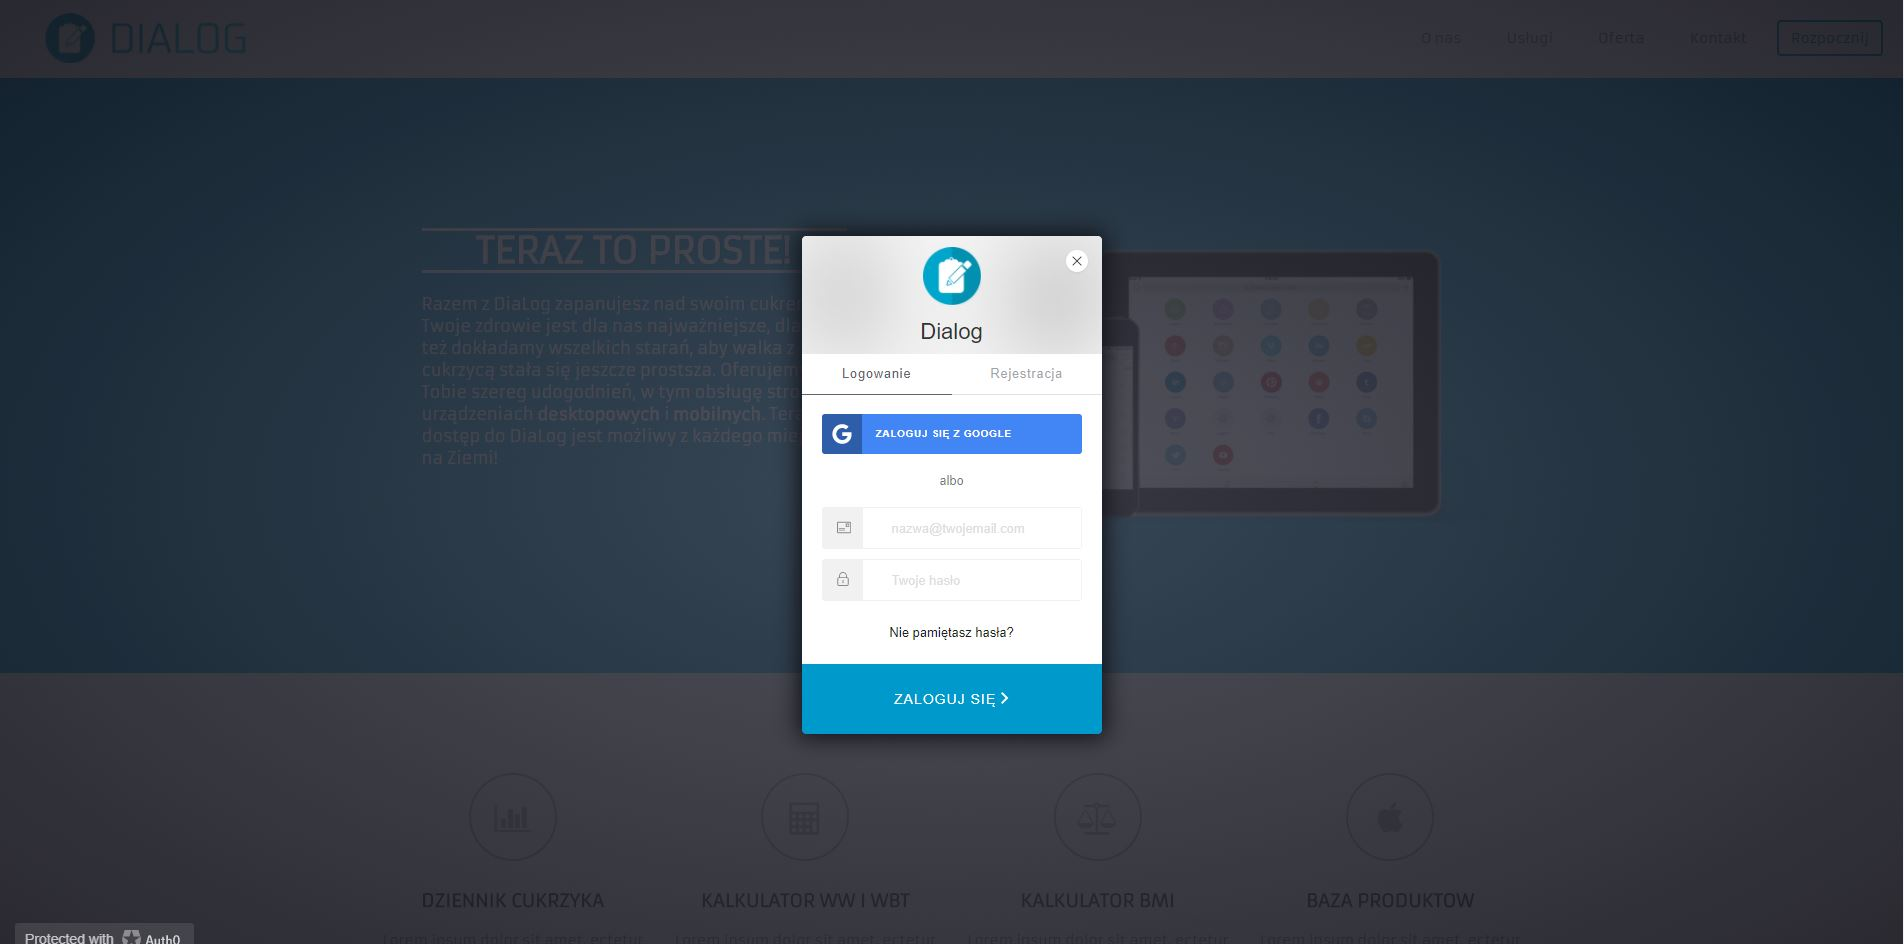
\includegraphics[scale=0.3]{images/logowanie_google.jpg}
	\caption{Okno logowania użytkownika}
	\label{Rys:logowanie}
\end{figure}

Po wpisaniu danych służących do logowania użytkownik uzyskuje dostęp do nowej pozycji w~ menu górnym -- \textit{Twój DiaLog}. Menu górne dostępne po zalogowaniu użytkownika zostało ukazane na rysunku  \ref{Rys:logged}.

\begin{figure}[h]
	\centering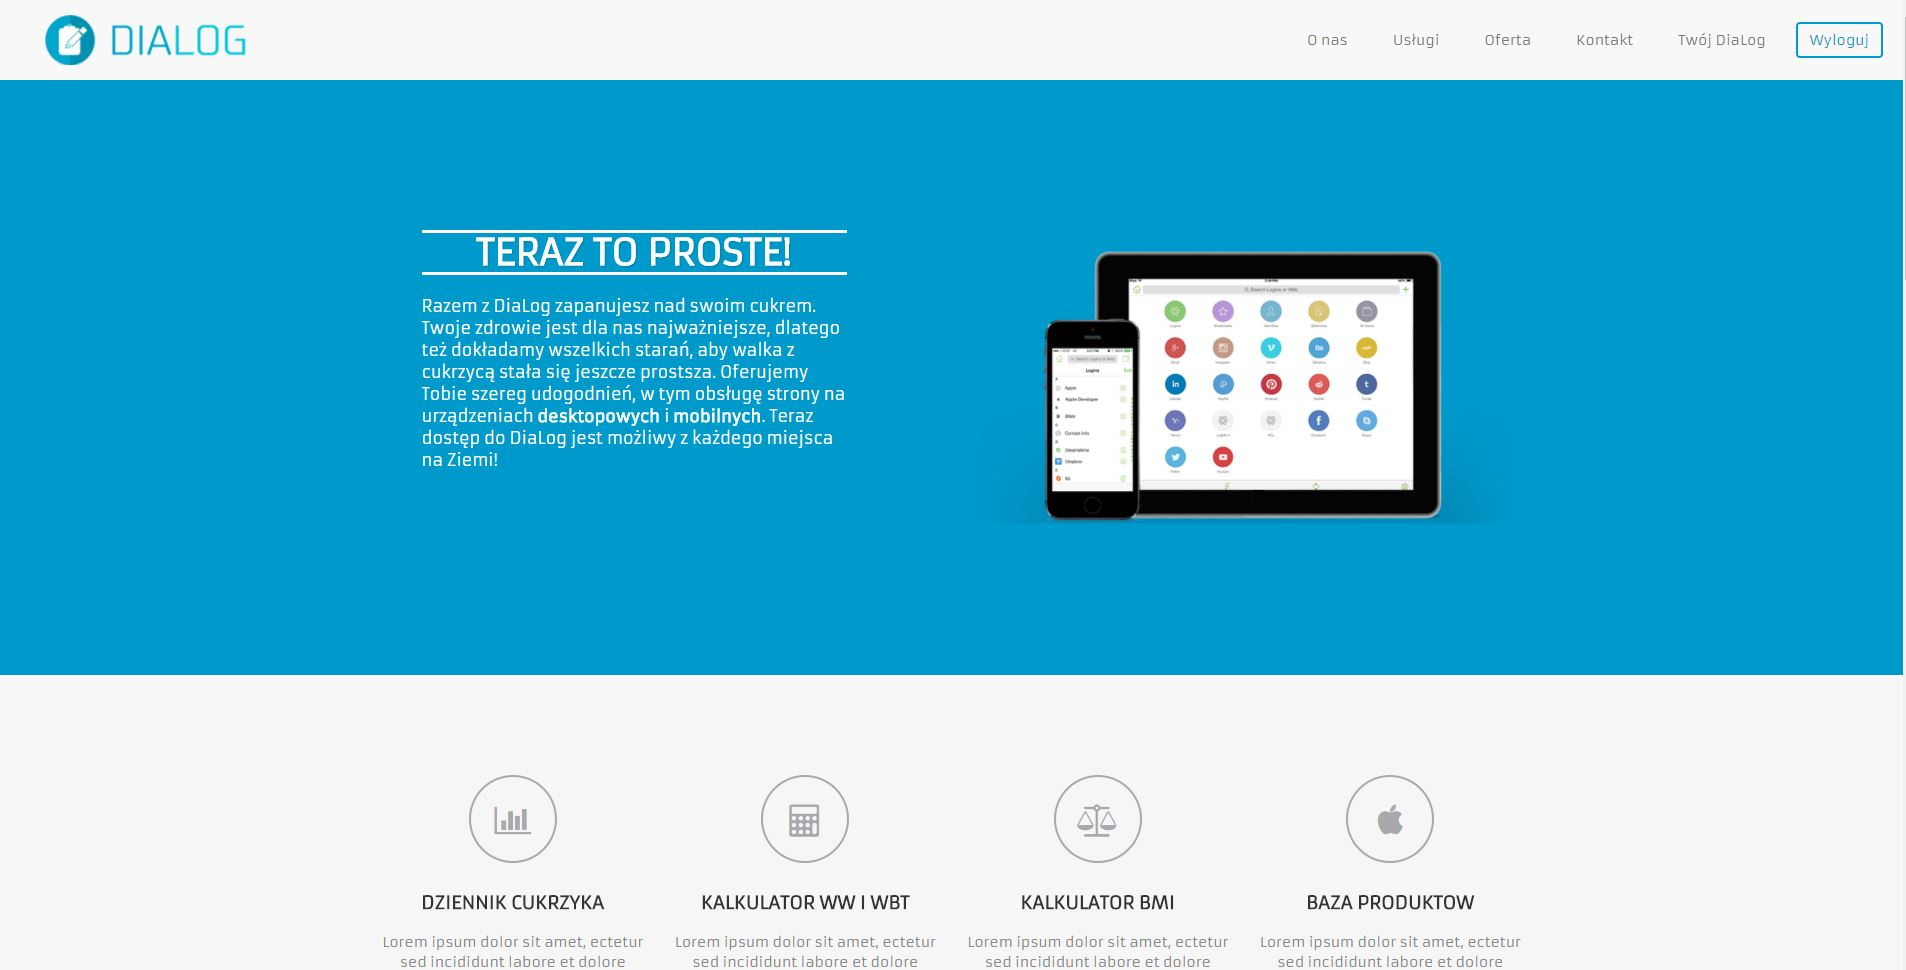
\includegraphics[scale=0.3]{images/ekran_logged.jpg}
	\caption{Menu górne rozszerzone o dodatkową pozycję -- \textit{Twój DiaLog}, dostępne po zalogowaniu użytkownika}
	\label{Rys:logged}
\end{figure}

\section{Użytkowanie panelu użytkownika zarejestrowanego}
Po uzyskaniu dostępu do zakładki \textit{Twój DiaLog} i kliknięciu jej, użytkownik uzyskuje dostęp do strony głównej panelu użytkownika zarejestrowanego będącej jednocześnie komponentem podsumowującym pomiary wprowadzone przez użytkownika. Początkowo, po rejestracji wykresy i tabela zestawień są puste, gdyż nie zawierają żadnych danych. Strona główna po kliknięciu pozycji górnego menu \textit{Twój DiaLog} została ukazana na rysunku \ref{Rys:firstPage}.

\begin{figure}[h]
	\centering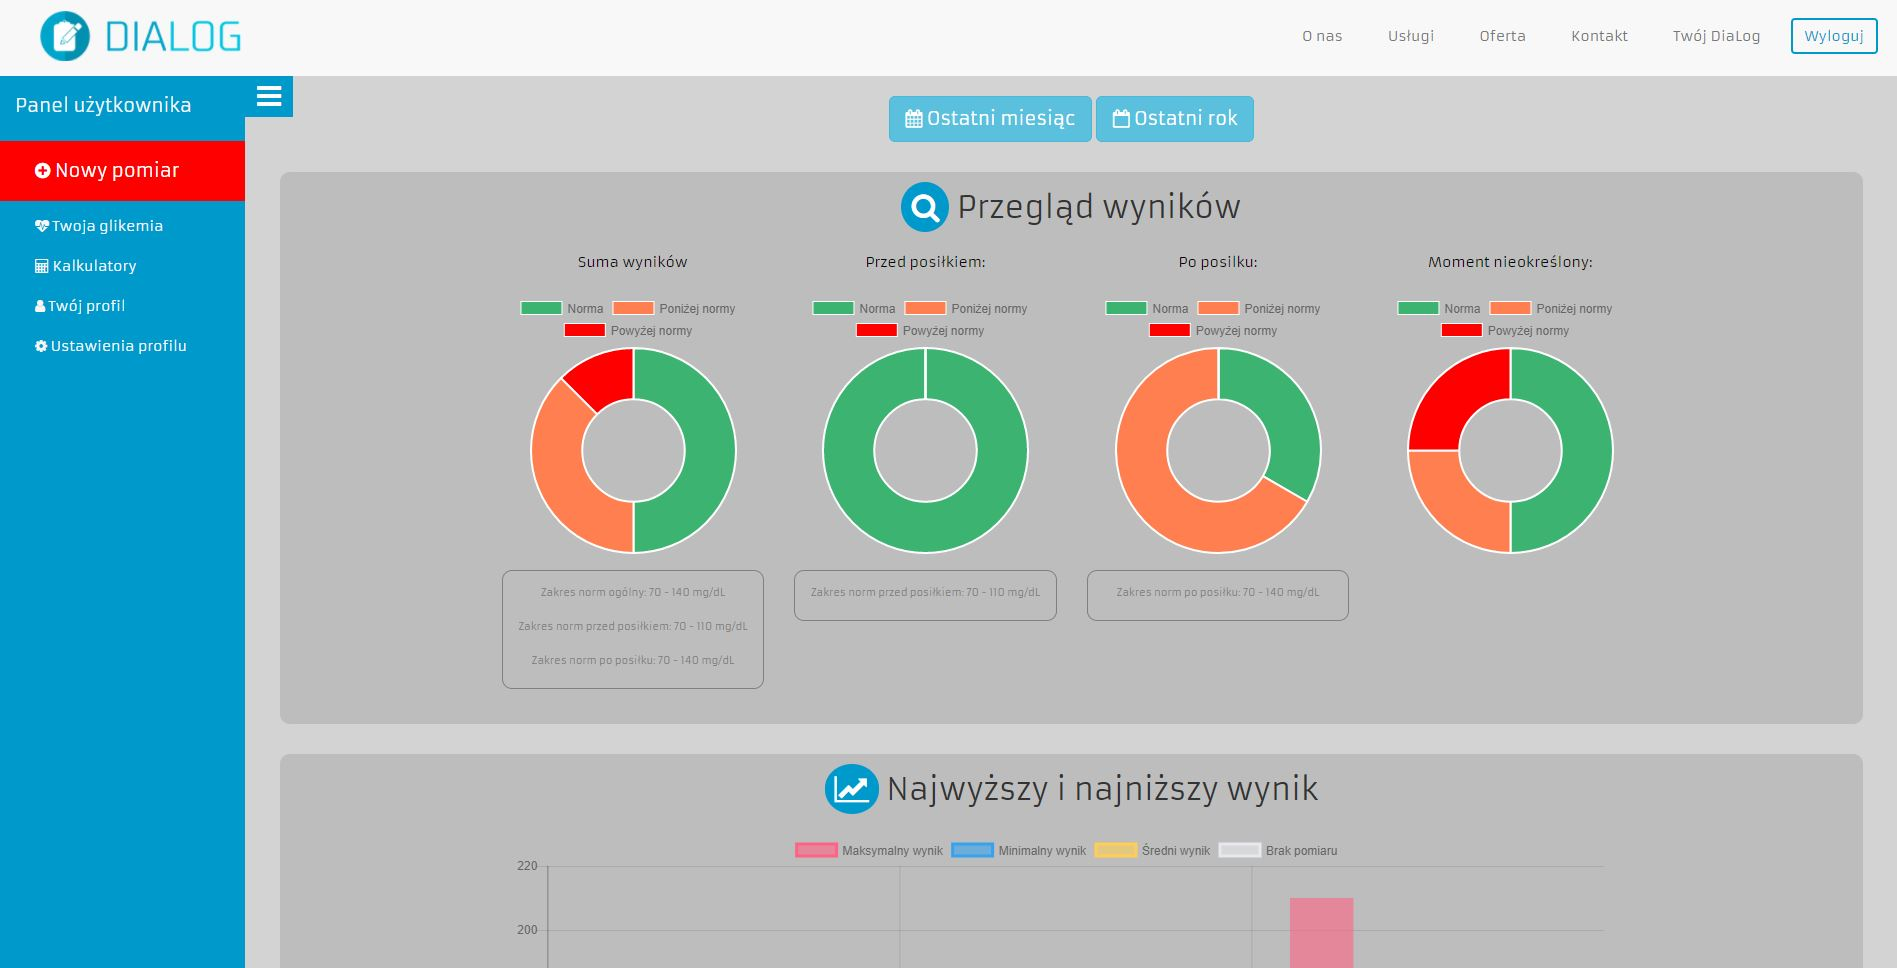
\includegraphics[scale=0.3]{images/first_page.jpg}
	\caption{Strona główna dostępna po kliknięciu przycisku menu górnego \textit{Twój DiaLog}, dostępnego po zalogowaniu użytkownika}
	\label{Rys:firstPage}
\end{figure}

\subsection{Twoja glikemia}
Zawartość dostępna z poziomu zakładki \textit{Twoja glikemia} wyświetlana jest jako strona główna po kliknięciu zakładki \textit{Twój DiaLog}. Zawiera ona wykresy kołowe podsumowujące ilość dodanych pomiarów glikemii. Każdy z czterech wykresów kołowych dotyczy odrębnego rodzaju pomiaru. Rodzaje pomiarów glikemii rozróżniane są w następujący sposób:

\begin{itemize}
	\item Przed posiłkiem,
	\item Po posiłku,
	\item Moment nieokreślony.
\end{itemize}

Pierwszy z wykresów jest sumą ilości pomiarów z pozostałych trzech wykresów. Ponadto, każdy z wykresów rozróżnia normy zakresu glikemii odpowiednie dla danego rodzaju pomiaru:

\begin{itemize}
	\item Przed posiłkiem:
	\begin{itemize}
		\item Norma ogólna: 70 - 140 mg/dL.
	\end{itemize}
	\item Po posiłku,
	\begin{itemize}
		\item Zakres norm przed posiłkiem: 70 - 110 mg/dL.
	\end{itemize}
	\item Moment nieokreślony.
	\begin{itemize}
		\item Zakres norm po posiłku: 70 - 140 mg/dL.
	\end{itemize}
\end{itemize}

Dla lepszej przejrzystości, do zaznaczenia norm na wykresie zostały użyte charakterystyczne kolory. Przy przekroczeniu normy wykres przyjmuje kolor czerwony. Jeżeli pomiar glikemii mieścił się w normie, wykres zostaje zaznaczony kolorem zielonym. W przypadku wartości glikemii znajdującej się poniżej normy wykres przyjmuje kolor pomarańczowy. Dodatkowo, po najechaniu kursorem na daną część wykresu użytkownikowi wyświetla się dymek z podpowiedzią ile pomiarów znajduje się w danym zakresie norm. 

\begin{figure}[h]
	\centering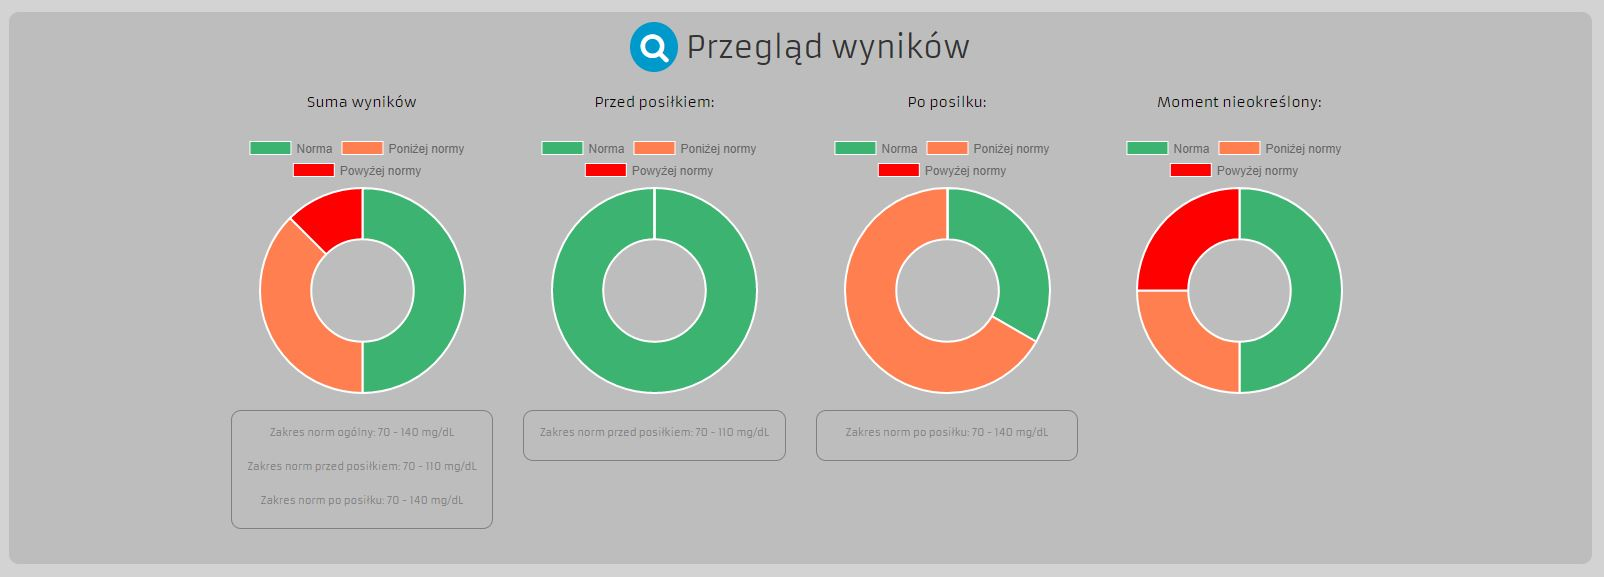
\includegraphics[scale=0.35]{images/bar_charts.jpg}
	\caption{Wykresy kołowe dostępne z poziomu zakładki \textit{Twoja glikemia}}.
	\label{Rys:barChart}
\end{figure}

Kolejnym elementem dostępnym z poziomu zakładki \textit{Twoja glikemia} są wykresy słupkowe. Zestawiają one maksymalny, minimalny oraz średni wynik dla każdego z rodzajów pomiarów glikemii. Po najechaniu na dany słupek wykresu użytkownik ma dostęp do informacji o wartości danego wyniku. 

\begin{figure}[h]
	\centering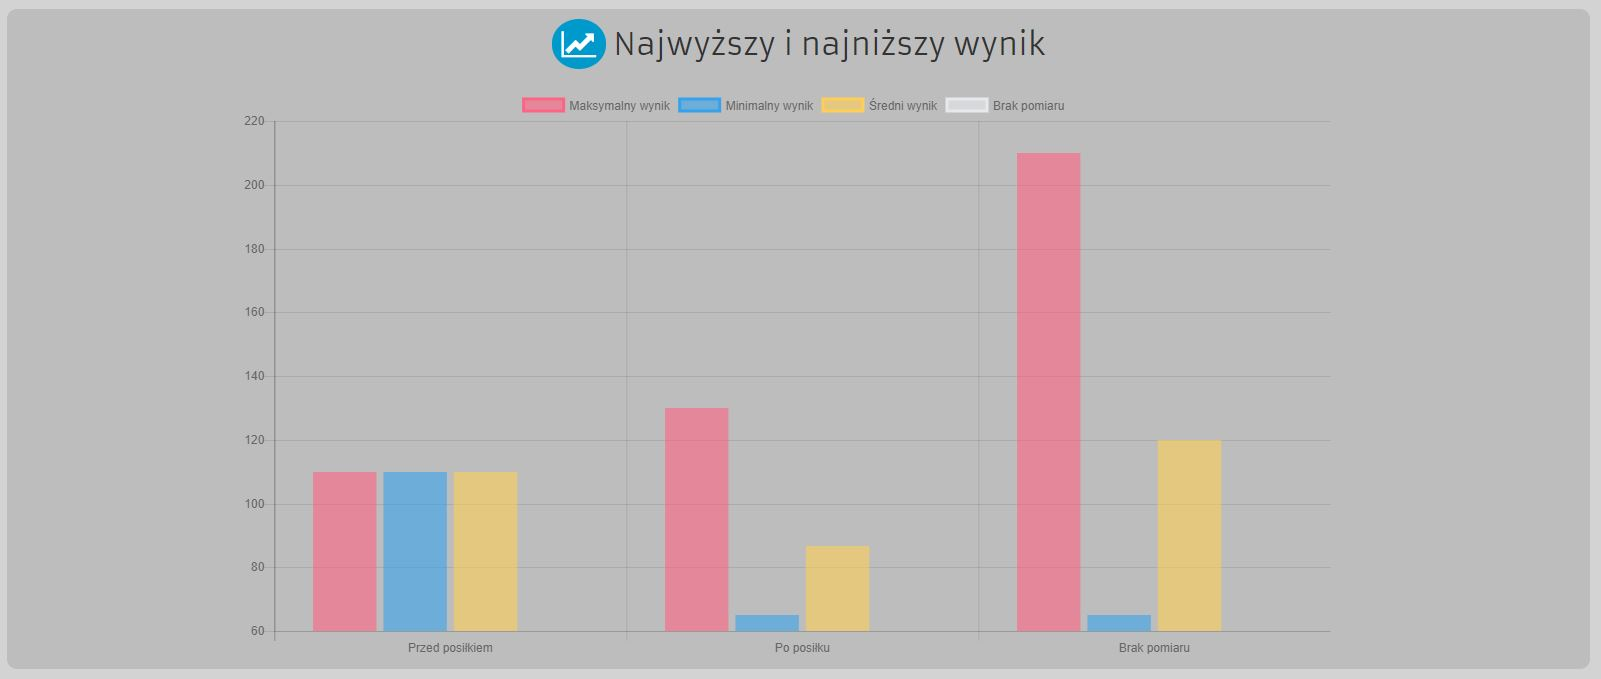
\includegraphics[scale=0.35]{images/normal_chart.jpg}
	\caption{Wykresy słupkowe dostępne z poziomu zakładki \textit{Twoja glikemia}}.
	\label{Rys:normalChart}
\end{figure}

Ostatnim z elementów zakładki \textit{Twoja glikemia} jest tabela zestawień. Podsumowuje ona (w~ zależności od pory dnia -- rano, południe, wieczór, noc) następujące dane: 

\begin{itemize}
	\item Liczba wyników, 
	\item Najwyższy wynik (mg/dL),
	\item Najniższy wynik (mg/dL),
	\item \% wyników powyżej normy,
	\item \% wyników poniżej normy,
	\item \% wyników w normie.
\end{itemize}

Ostatnia kolumna tabeli przedstawia sumę wyników danego wiersza. 

\begin{figure}[h]
	\centering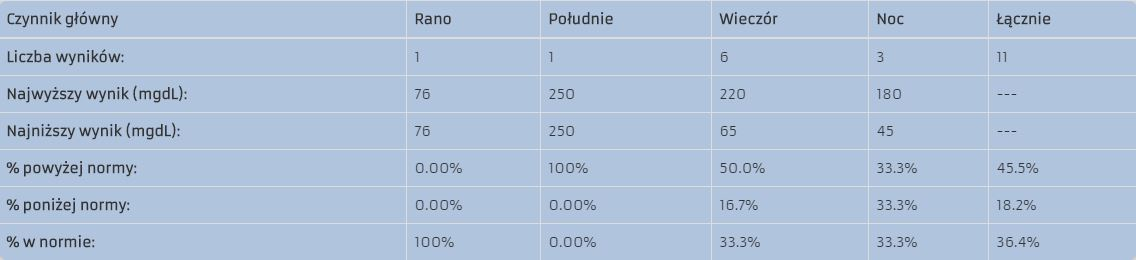
\includegraphics[scale=0.5]{images/table.jpg}
	\caption{Tabela zestawień pomiarów glikemii dostępna z poziomu zakładki \textit{Twoja glikemia}}.
	\label{Rys:table}
\end{figure}

Użytkownik ma możliwość wybrania przedziału czasu, na podstawie którego wyświetlane mają być dane. Dostępne są dwie opcje -- \textit{Ostatni miesiąc} oraz \textit{Ostatni rok}. Wyboru dokonuje się poprzez kliknięcie jednego z dwóch dostępnych przycisków na szczycie podstrony.

\newpage

\subsection{Dodaj pomiar}
Zakładka \textit{Dodaj pomiar} otwiera okno modalne dodawania nowego pomiaru (rys. \ref{Rys:measurement}). Z poziomu tego okna użytkownik wprowadza dane, które zestawiane są później na stronie komponentu \textit{Twoja glikemia} w postaci wykresów i tabeli zestawień:

\begin{itemize}
	\item Data i godzina pomiaru,
	\item Wartość glikemii,
	\item Moment pomiaru,
	\item Krótka notatka.
\end{itemize}
Po naciśnięciu przycisku \textit{Dodaj} zostaje dodany do bazy danych pomiarów nowy pomiar.  

\begin{figure}[h]
	\centering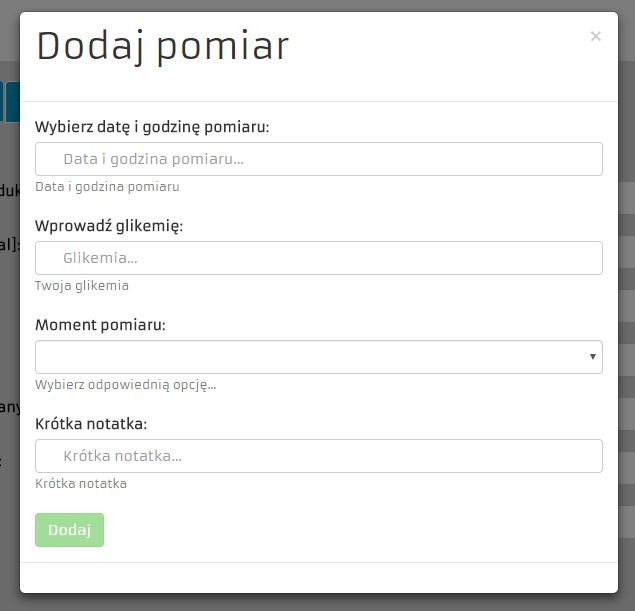
\includegraphics[scale=0.5]{images/measurement.jpg}
	\caption{Okno modalne dodawania nowego pomiaru}
	\label{Rys:measurement}
\end{figure}

\subsection{Kalkulatory}
Zakładka \textit{Kalkulatory} pozwala użytkownikowi na uzyskanie dostępu do kalkulatora \textit{BMI (Body Mass Index)} oraz do kalkulatora wymienników węglowodanowych oraz białkowo~-tłuszczowych, dostępnego wraz z tabelą makroskładników produktów spożywczych pochodzących z bazy danych produktów. 
Kalkulator \textit{BMI (Body Mass Index)} pozwala obliczyć współczynnik masy do wzrostu. Składa się on z dwóch pól typu 
\textit{Input}. W pierwszym z~ nich użytkownik wpisuje swoją wagę, a~ w następnym wzrost (rys. \ref{Rys:bmiBefore}). Po~ kliknięciu przycisku \textit{Oblicz} użytkownik otrzymuje informację o uzyskanym wyniku współczynnika \textit{BMI} oraz podpowiedź do jakiej grupy osób (ze względu na wagę) się zalicza (rys. \ref{Rys:bmiAfter}):

\begin{itemize}
	\item osoby z niedowagą,
	\item osoby z wagą prawidłową,
	\item osoby z nadwagą,
	\item osoby z otyłością I stopnia,
	\item osoby z otyłością II stopnia,
	\item osoby z otyłością III stopnia.
\end{itemize}

\begin{figure}[h]
	\centering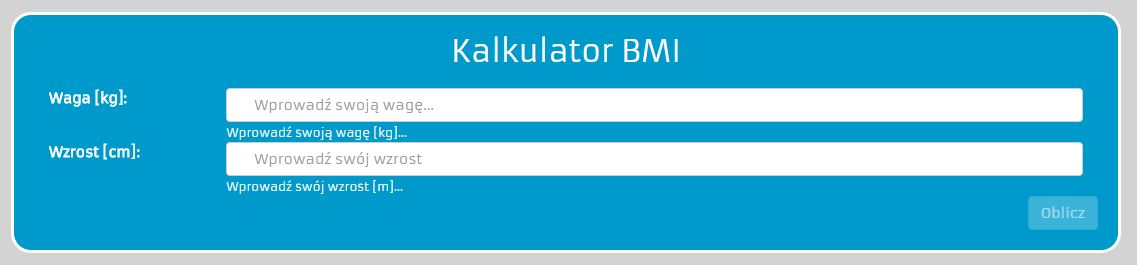
\includegraphics[scale=0.5]{images/bmi_before.jpg}
	\caption{Interfejs kalkulatora BMI}.
	\label{Rys:bmiBefore}
\end{figure}

\begin{figure}[h]
	\centering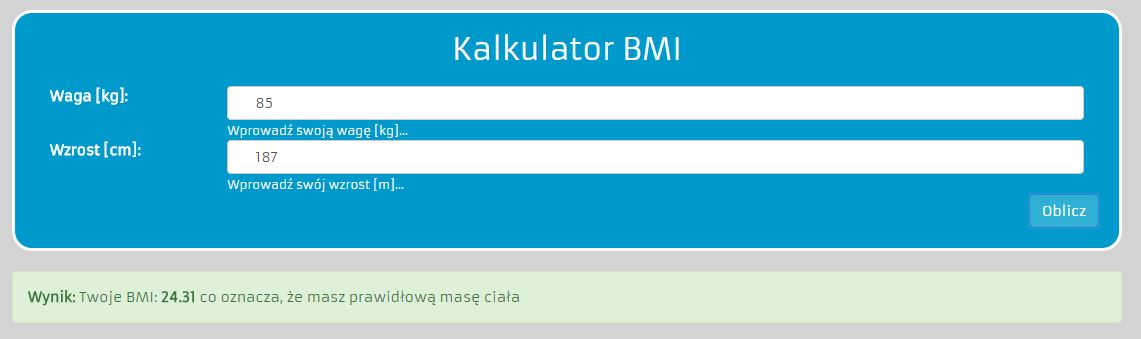
\includegraphics[scale=0.5]{images/bmi_after.jpg}
	\caption{Interfejs kalkulatora BMI po uzyskaniu wyniku}.
	\label{Rys:bmiAfter}
\end{figure}

Kolejną funkcjonalnością dostępną z poziomu zakładki \textit{Kalkulatory} menu bocznego jest kalkulator wymienników węglowodanowych i wymienników białkowo-tłuszczowych na podstawie tabeli makroskładników produktów dostępnych z poziomu tabeli \textit{products}, która może być stale rozszerzana przez zalogowanych użytkowników aplikacji (rys. \ref{Rys:wwBefore}). Wynik przedstawiany jest w postaci kolumn dołączonych do tabeli makroskładników danego produktu. Aby obliczyć wartość wymienników węglodowanowych i wymienników białkowo-tłuszczowych należy wybrać dany produkt poprzez wpisanie ciągu (bądź części ciągu) znaków w polu formularza o nazwie \textit{Wybierz produkt}. Do tego pola przypięty jest inteligentny moduł wyszukiwania znajdujący produkty po słowach kluczowych. Po wpisaniu części wyrazu moduł podpowiada użytkownikowi najbardziej prawdopodobne wyniki w~ postaci listy rozwijanej. Dodatkowo użytkownik ma możliwość podania porcji produktu w polu \textit{Wpisz wagę produktu [g]}. Wartości makroskładników i wyników obliczonych przez kalkulatory są wówczas dynamicznie zmieniane w zależności od wpisanej porcji produktu. Domyślna wartość pola to 100 [g]. 

Dodatkowo, jako ostatnia kolumna tabeli dodana została informacja czy produkt może być szkodliwy dla zdrowia osoby chorej na cukrzycę czy też nie. System rekomendacji oparty jest na ilości węglowodanów zawartych w produkcie. Jeżeli w 100 gramach produktu, 50 gram to węglowodany, wówczas produkt może okazać się szkodliwy w diecie cukrzyka (rys. \ref{Rys:wwAfter}). 

\begin{figure}[h]
	\centering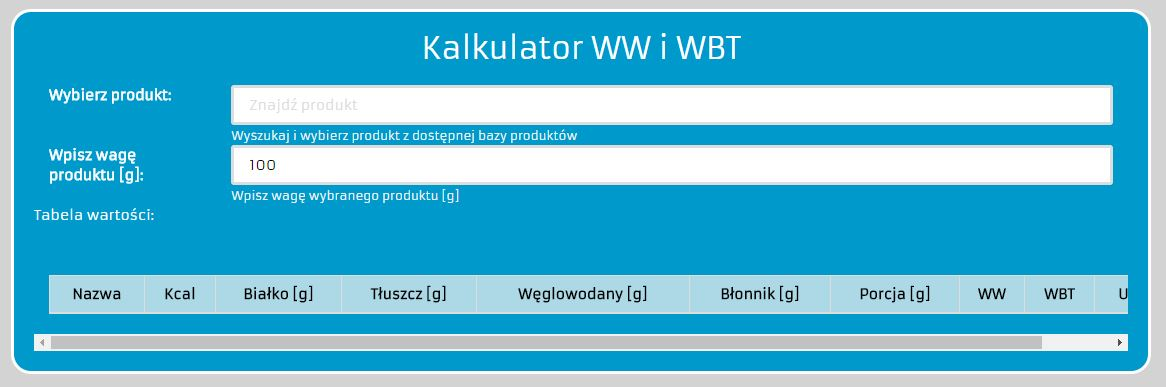
\includegraphics[scale=0.5]{images/ww_before.jpg}
	\caption{Interfejs kalkulatora wymienników węglowodanowych i~ białkowo-tłuszczowych}.
	\label{Rys:wwBefore}
\end{figure}

\begin{figure}[h]
	\centering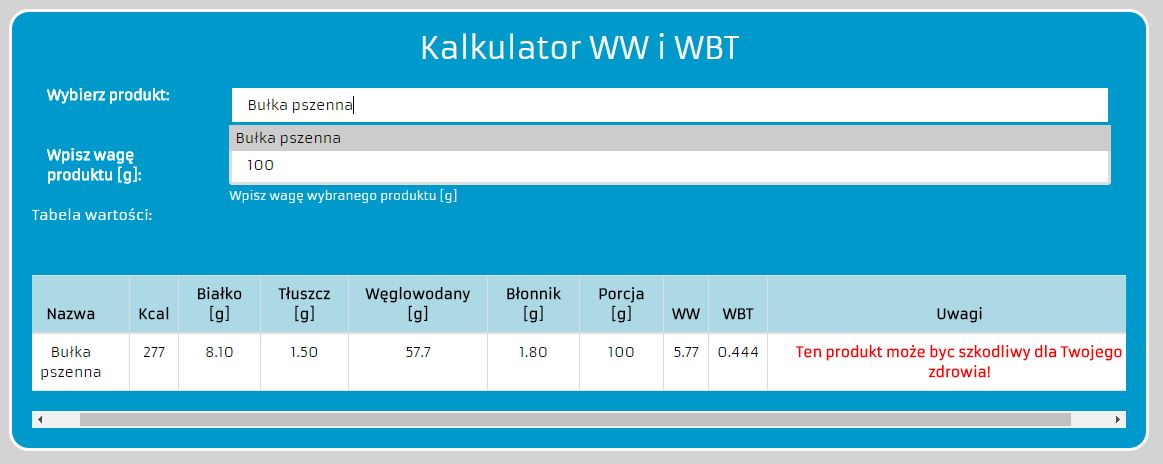
\includegraphics[scale=0.5]{images/ww_after.jpg}
	\caption{Interfejs kalkulatora wymienników węglowodanowych i~ białkowo-tłuszczowych po uzyskaniu wyniku}.
	\label{Rys:wwAfter}
\end{figure}

\newpage

Użytkownik zarejestrowany ma również możliwość dodawania produktów do bazy danych produktów. Formularz dodawania nowego produktu dostępny jest również z poziomu zakładki \textit{Twoja glikemia} -- karta \textit{Dodaj produkt} (rys. \ref{Rys:addProduct}). 

\begin{figure}[h]
	\centering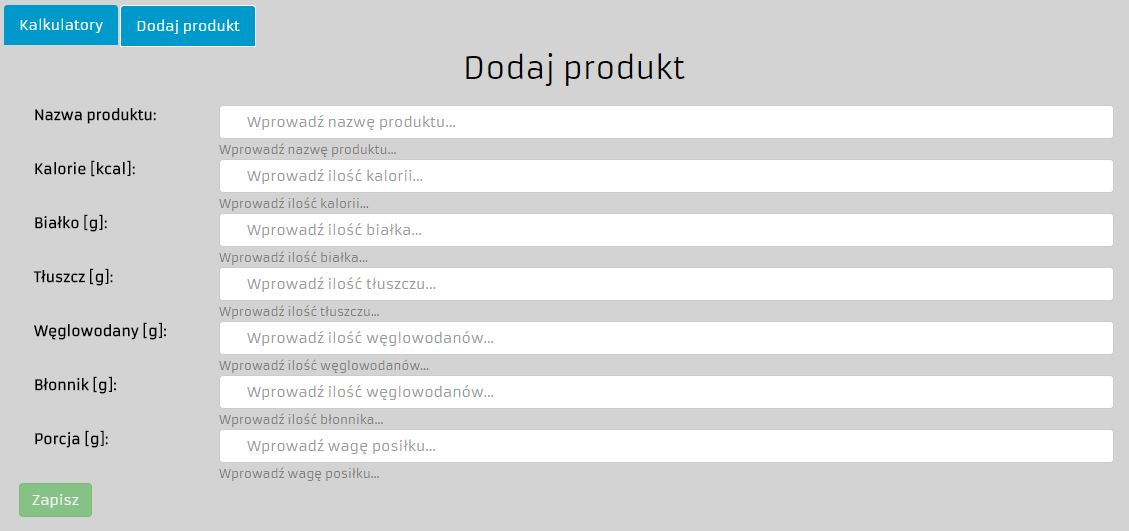
\includegraphics[scale=0.5]{images/add_product.jpg}
	\caption{Formularz dodawania nowego produktu}.
	\label{Rys:addProduct}
\end{figure}

Po wypełnieniu wszystkich pól: 
\begin{itemize}
	\item Nazwa produktu,
	\item Kalorie [kcal],
	\item Białko [g],
	\item Tłuszcz [g],
	\item Węglowodany [g],
	\item Błonnik [g],
	\item Porcja [g]
\end{itemize}
produkt jest dynamicznie dodawany do bazy danych i bezpośrednio dostępny z pozycji modułu kalkulatora do obliczania wymienników węglowodanowych i białkowo-tłuszczowych.

\subsection{Twój profil}
Z poziomu zakładki \textit{Twój profil} użytkownik ma możliwość dodania informacji zarówno o profilu (rys. \ref{Rys:yourProfile}) jak i danych medycznych (rys. \ref{Rys:medicalData}). Czynność ta odbywa się przy pomocy dwóch formularzy z odpowiednimi polami:

\begin{itemize}
	\item Dla karty \textit{Twój profil}
	\begin{itemize}
		\item imię,
		\item nazwisko,
		\item PESEL,
		\item opiekun -- lista rozwijana,
		\item ulica,
		\item nr domu,
		\item miasto,
		\item kod pocztowy,
		\item numer telefonu,
		\item aktualny glukometr -- lista rozwijana,
		\item poprzedni glukometr -- lista rozwijana,
		\item numer seryjny glukometru.
	\end{itemize}
	\item Dla karty \textit{Dane medyczne}
	\begin{itemize}
		\item typ cukrzycy -- lista rozwijana,
		\item rok zachorowania -- lista rozwijana,
		\item rodzaj insuliny -- lista rozwijana,
		\item przyjmowany lek -- lista rozwijana,
		\item inne leki i insuliny,
		\item BMI,
		\item wzrost,
		\item waga,
		\item hBA1c.
	\end{itemize}
\end{itemize}

Przy pierwszym wpisaniu danych do wszystkich pól formularza i zatwierdzeniu ich przyciskiem \textit{Zapisz}, zostanie wykonana operacja zapisania danych do obydwu tabel bazy danych. Przy każdorazowym otwarciu zakładki \textit{Twój profil} dane te będą czytane z bazy danych do pól formularza. W~ przypadku chęci zaktualizowania informacji użytkownik nadpisuje pola formularza nowymi danymi i wykonywana jest operacja \textit{UPDATE} zarówno w przypadku jednej, jak i drugiej tabeli.

\begin{figure}[h]
	\centering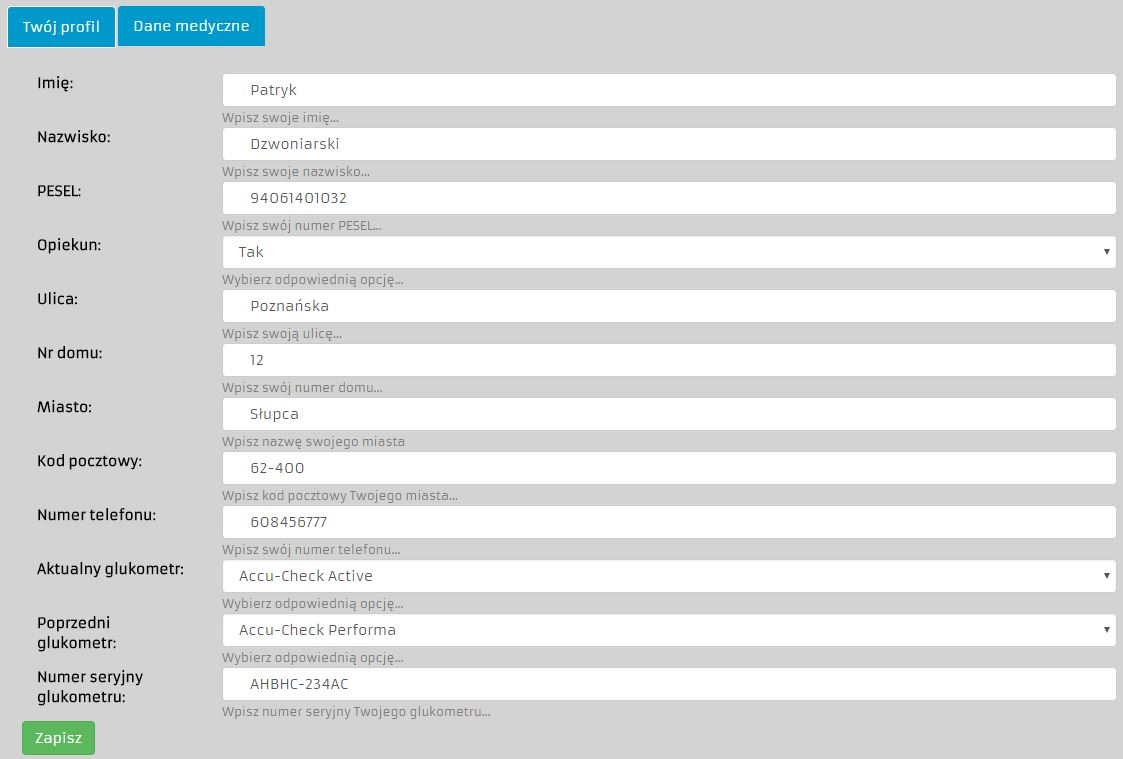
\includegraphics[scale=0.5]{images/yourprofile.jpg}
	\caption{Formularz dodawania i aktualizacji informacji o profilu}
	\label{Rys:yourProfile}
\end{figure}

\newpage

\begin{figure}[h]
	\centering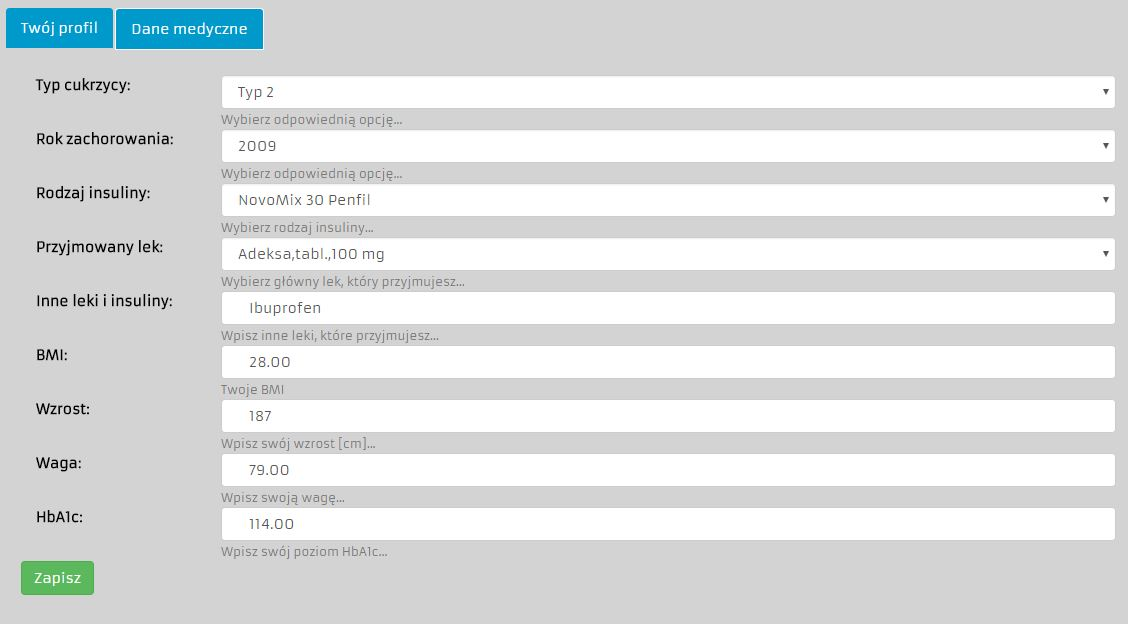
\includegraphics[scale=0.5]{images/medical_data.jpg}
	\caption{Formularz dodawania i aktualizacji danych medycznych użytkownika profilu}
	\label{Rys:medicalData}
\end{figure}

\subsection{Ustawienia profilu}
W zakładce \textit{Ustawienia profilu} użytkownik ma możliwość dodania, bądź zaktualizowania bieżących zakresów glikemii (rys. \ref{Rys:profileSettings}). Komponent składa się z trzech pól formularza:

\begin{itemize}
	\item Hipoglikemia, 
	\item Hiperglikemia,
	\item Hiperglikemia po posiłku.
\end{itemize}

\begin{figure}[h]
	\centering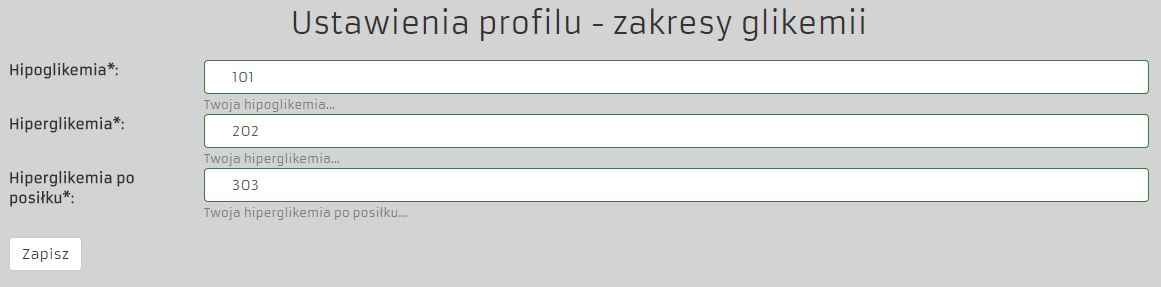
\includegraphics[scale=0.5]{images/profile_settings.jpg}
	\caption{Formularz dodawania i aktualizacji danych dotyczących zakresów glikemii użytkownika}
	\label{Rys:profileSettings}
\end{figure}


Każde pole może być w dowolnym czasie aktualizowanie (operacja \textit{UPDATE}) w bazie danych. Ponadto dane wczytywane są bezpośrednio do pól formularza przy użyciu metody \textit{GET}. 
\chapter{Panel użytkownika niezarejestrowanego oraz niezalogowanego}

\section{Okno rejestracji użytkownika}
W poniższej sekcji ukazany zostanie interfejs programu umożliwiający użytkownikowi niezarejestrowanemu w systemie dokonania rejestracji. Rejestracja przebiegać może w~ dwóch wariantach:
\begin{itemize}
	\item Rejestracja przy użyciu konta \textit{Google},
	\item Rejestracja tradycyjna -- podanie adreu e-mail oraz hasła.
\end{itemize}

\subsection{Rejestracja przy użyciu konta \textit{Google}}
Opcja rejestracji i logowania za pomocą konta \textit{Google} znacznie ułatwia i przyspiesza proces dodawania nowego użytkownika. Pozwala ona zwiększyć odsetek nowych użytkowników systemu. Kolejnym powodem, który przemawia za tym, aby stosować logowanie przy użyciu danych pochodzących z portali społecznościowych jest fakt mówiący o tym, że adres e-mail, którym posługuje się dana osoba w momencie takiej rejestracji został już wcześniej zweryfikowany przez dostawcę sieci społecznościowej. Oznacza to, że w momencie logowania przy użyciu konta społecznościowego otrzymujemy rzetelne informacje, a~ nie fałszywe adresy, które użytkownicy wykorzystują zazwyczaj do zarejestrowania się na stronach internetowych. 

Cały proces rejestracji i pózniejszego logowania się do aplikacji przy użyciu konta \textit{Google} przebiega w następujący sposób: 
\begin{itemize}
	\item użytkownik wybiera opcję rejestracji w systemie i klika przycisk \textit{Zaloguj się za pomocą konta} \textit{Google} (rys. \ref{Rys:register}) i wpisuje dane logowania do konta \textit{Google}, bądź w~ przypadku kiedy jest zalogowany globalnie, wybiera odpowiednie konto (rys. \ref{Rys:choose_google}),
	\item żądanie rejestracji/logowania wysyłane jest do dostawcy sieci społecznościowej \textit{Google},
	\item w momencie gdy dostawca sieci społecznościowej \textit{Google} potwierdzi tożsamość użytkownika, bieżący użytkownik uzyskuje dostęp do aplikacji.
\end{itemize}

\newpage

\begin{figure}[h]
	\centering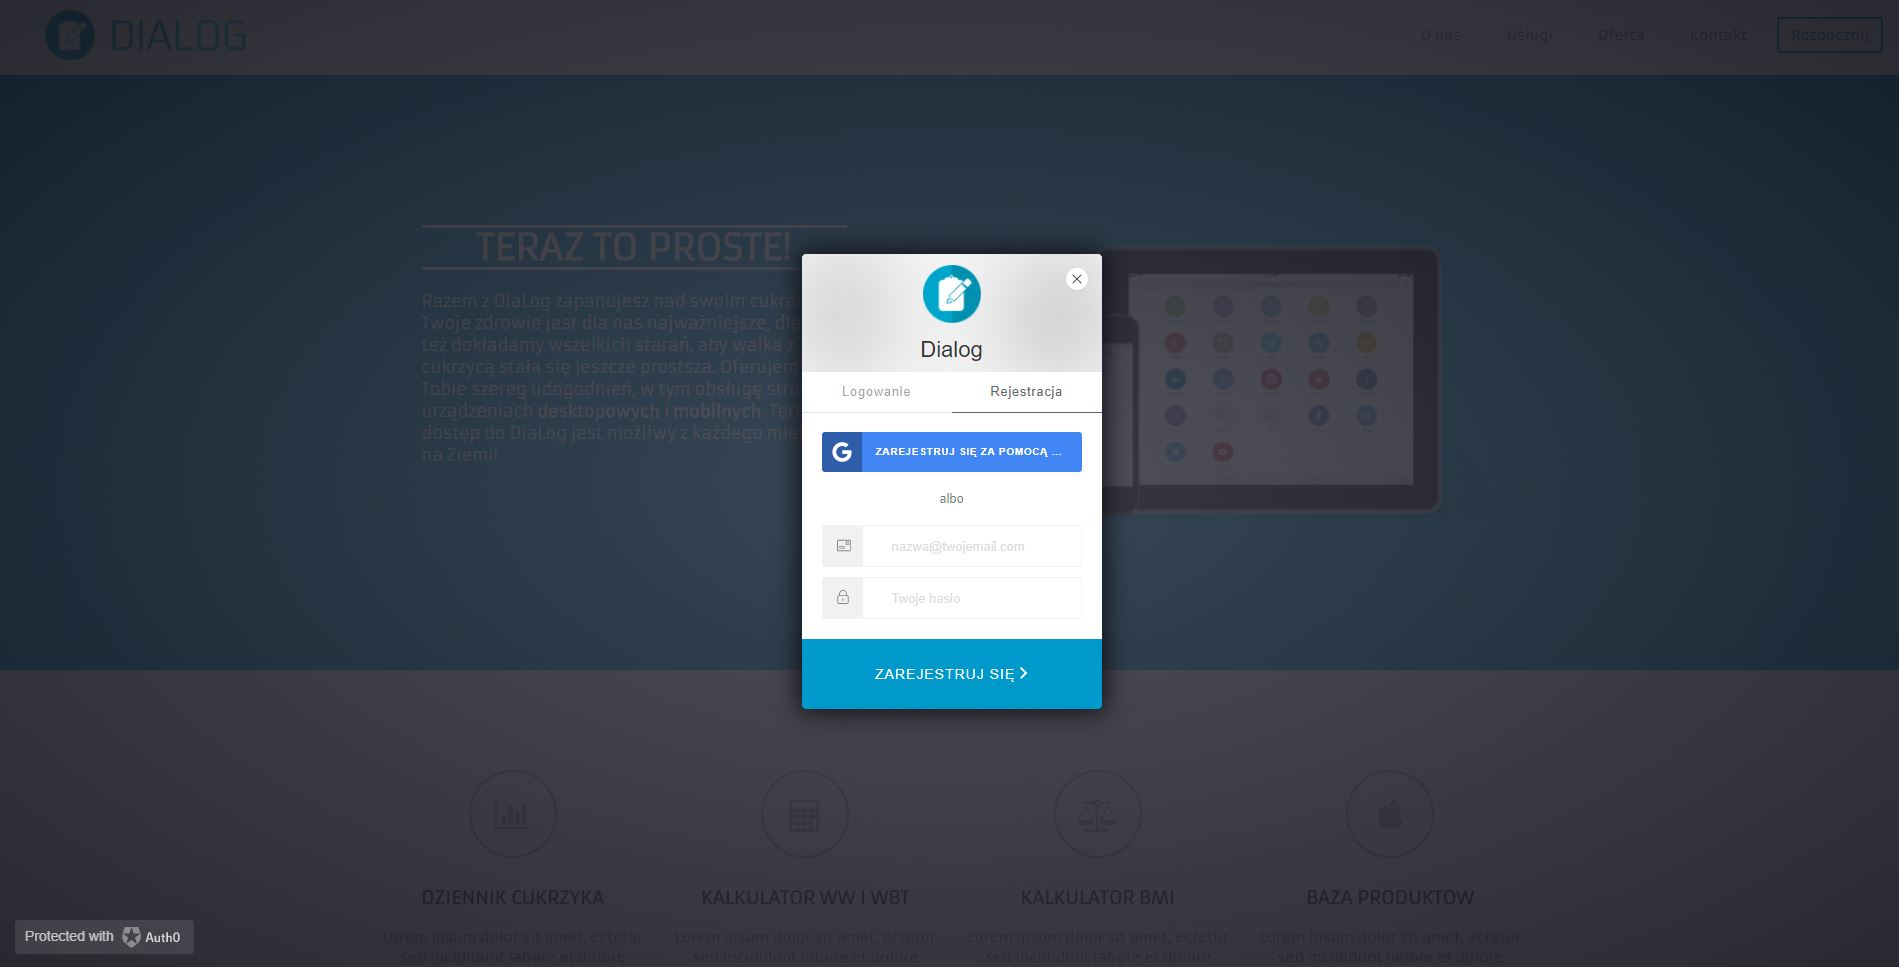
\includegraphics[scale=0.3]{images/register.jpg}
	\caption{Okno rejestracji użytkownika do systemu}
	\label{Rys:register}
\end{figure}

\begin{figure}[h]
	\centering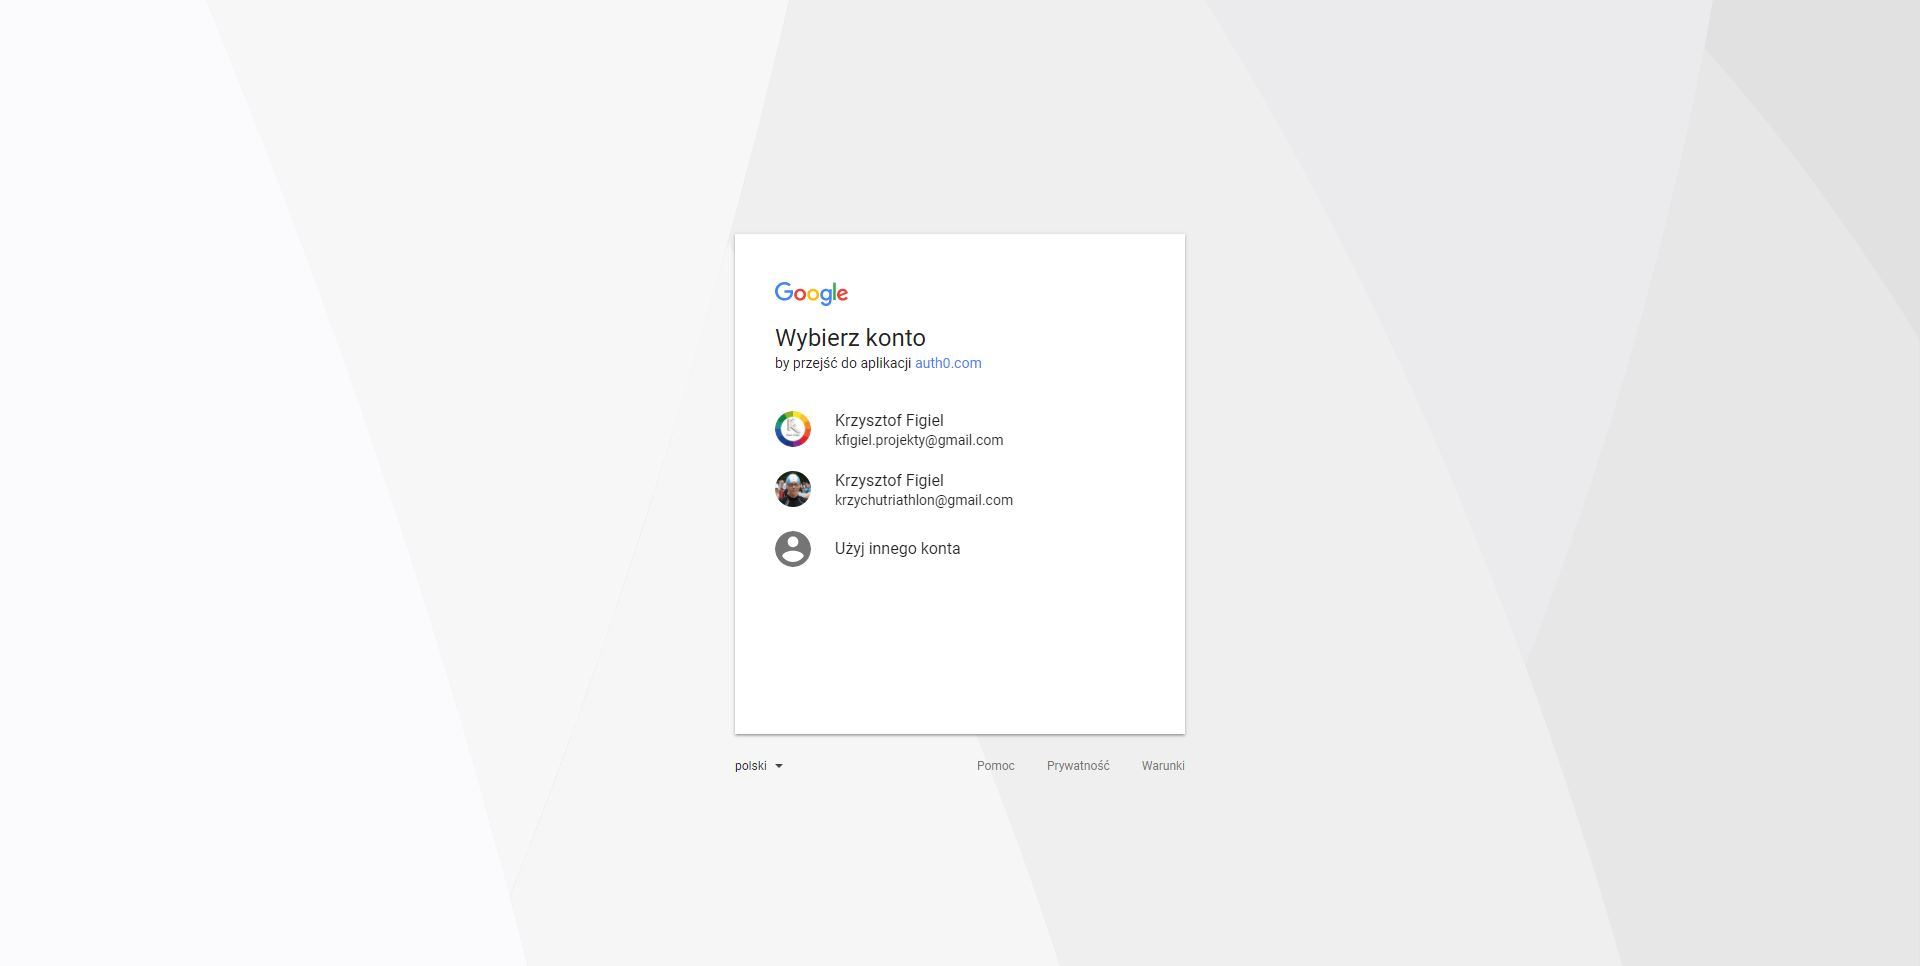
\includegraphics[scale=0.3]{images/google_account.jpg}
	\caption{Okno wyboru konta \textit{Google}}
	\label{Rys:choose_google}
\end{figure}

\subsection{Rejestracja tradycyjna -- podanie adreu e-mail oraz hasła}
W przypadku rejestracji tradycyjnej dane podane przez użytkownika (adres e-mail oraz hasło) zostają zapisane w zewnętrznej bazie danych dostawcy usług autoryzacji -- \textit{Auth0}. Po kliknięciu przycisku \textit{Zarejestruj się} (rys. \ref{Rys:normal_registration}) użytkownik zostaje powiadomiony o~ konieczności potwierdzenia autentyczności konta poprzez kliknięcie w link aktywacyjny wysłany automatycznie w wiadomości e-mail przez serwis \textit{Auth0} (rys. \ref{Rys:email_notification}). Po kliknięciu w link aktywacyjny możliwe jest już zalogowanie się. 

\newpage

\begin{figure}[h]
	\centering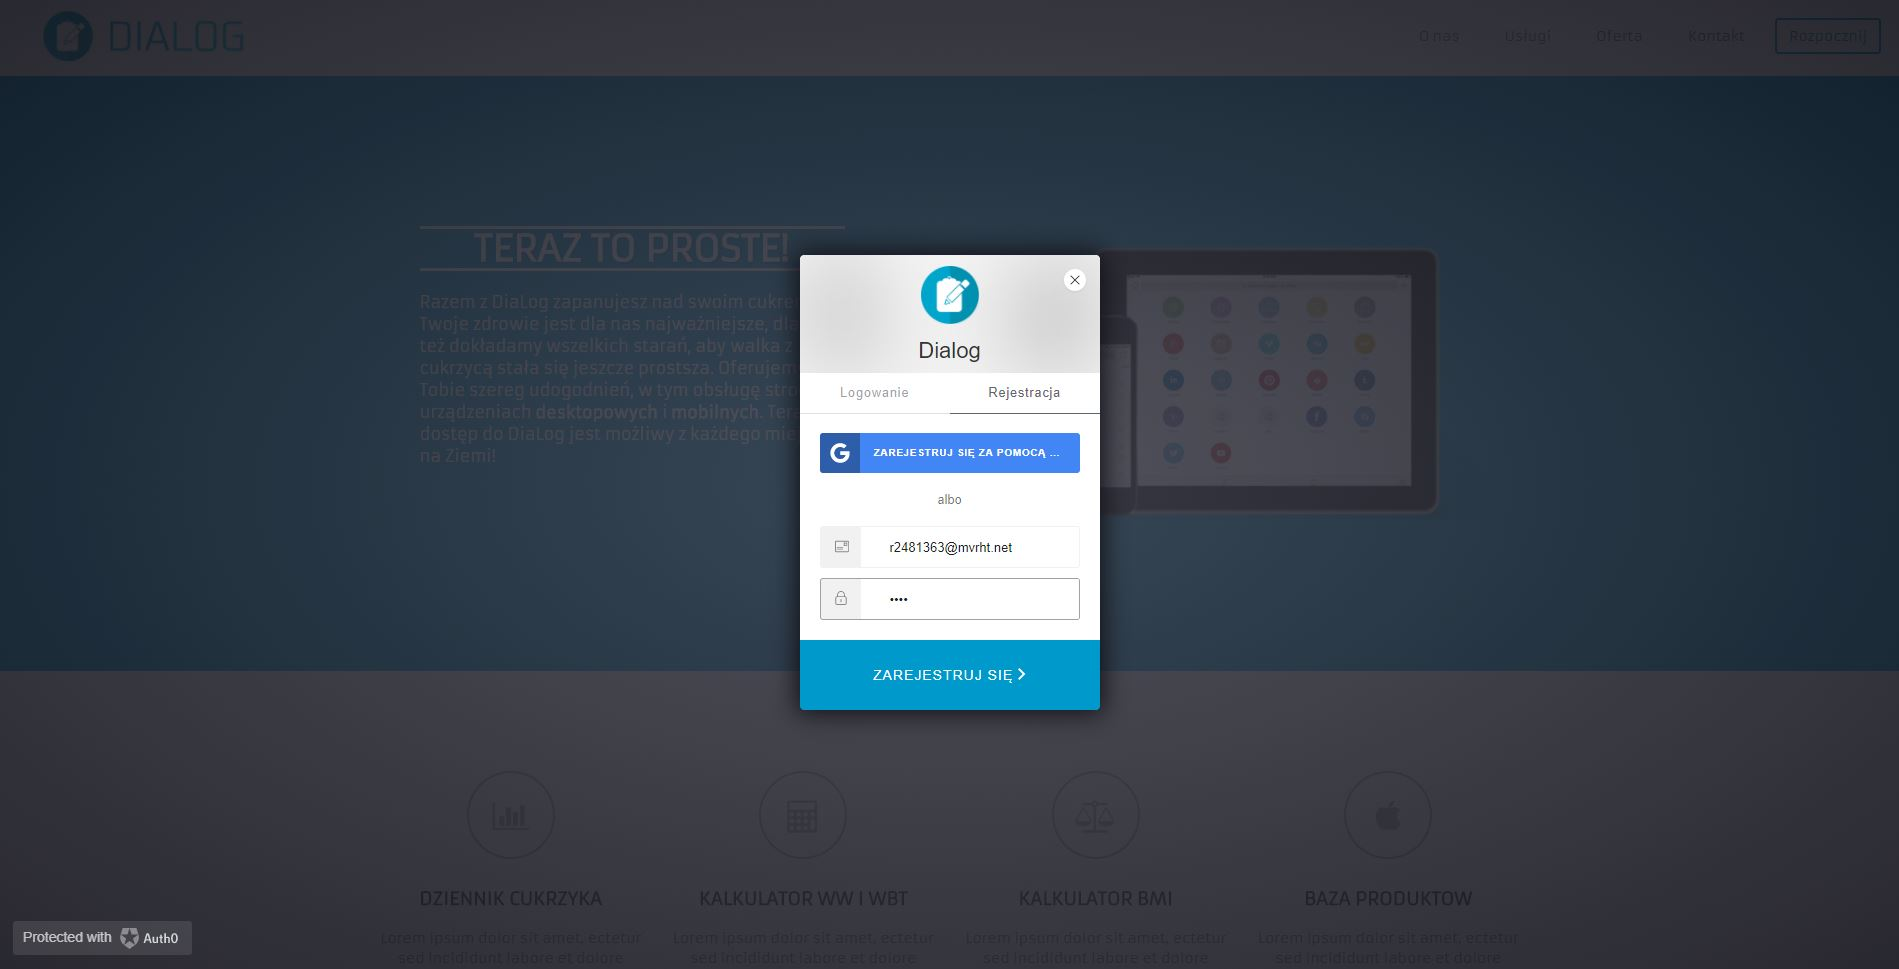
\includegraphics[scale=0.3]{images/normal_registration.jpg}
	\caption{Okno rejestracji tradycyjnej}
	\label{Rys:normal_registration}
\end{figure}

\begin{figure}[h]
	\centering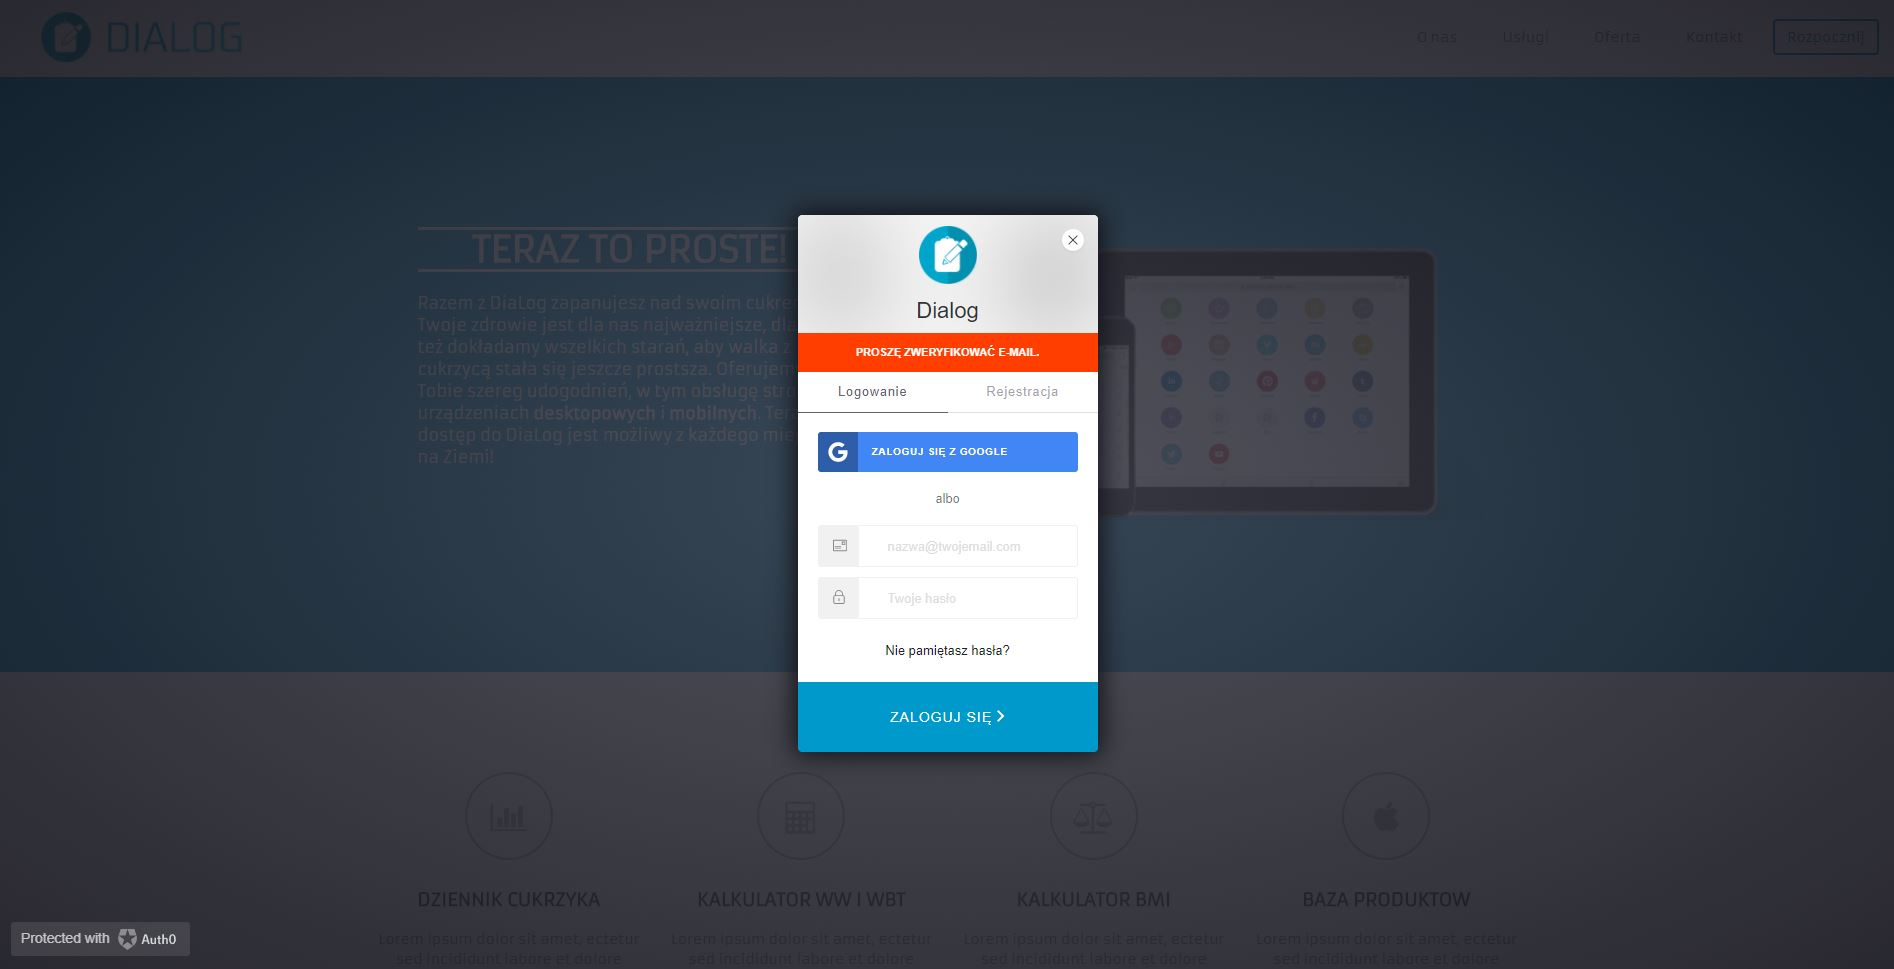
\includegraphics[scale=0.3]{images/email_verify.jpg}
	\caption{Okno z prośbą o potwierdzenie adresu e-mail}
	\label{Rys:email_notification}
\end{figure}

Po poprawnej rejestracji i późniejszym zalogowaniu się użytkownik ma dostęp do panelu użytkownika zarejestrowanego. Z poziomu panelu użytkownika niezalogowanego możliwe jest również uzyskanie informacji na temat funkcjonalności strony oraz wysłanie maila z zapytaniem do administracji za pomocą wbudowanego formularza z podpiętym modułem do wysyłania wiadomości e-mail. 

\newpage

Użytkownik może w każdej chwili wypełnić wymagane pola oraz wysłać wiadomość do administracji z dowolnym zapytaniem, klikając przycisk \textit{Wyślij} (rys. \ref{Rys:email_module}):
\begin{itemize}
	\item Imię,
	\item Nazwisko,
	\item Temat,
	\item Wiadomość
\end{itemize}

\begin{figure}[h]
	\centering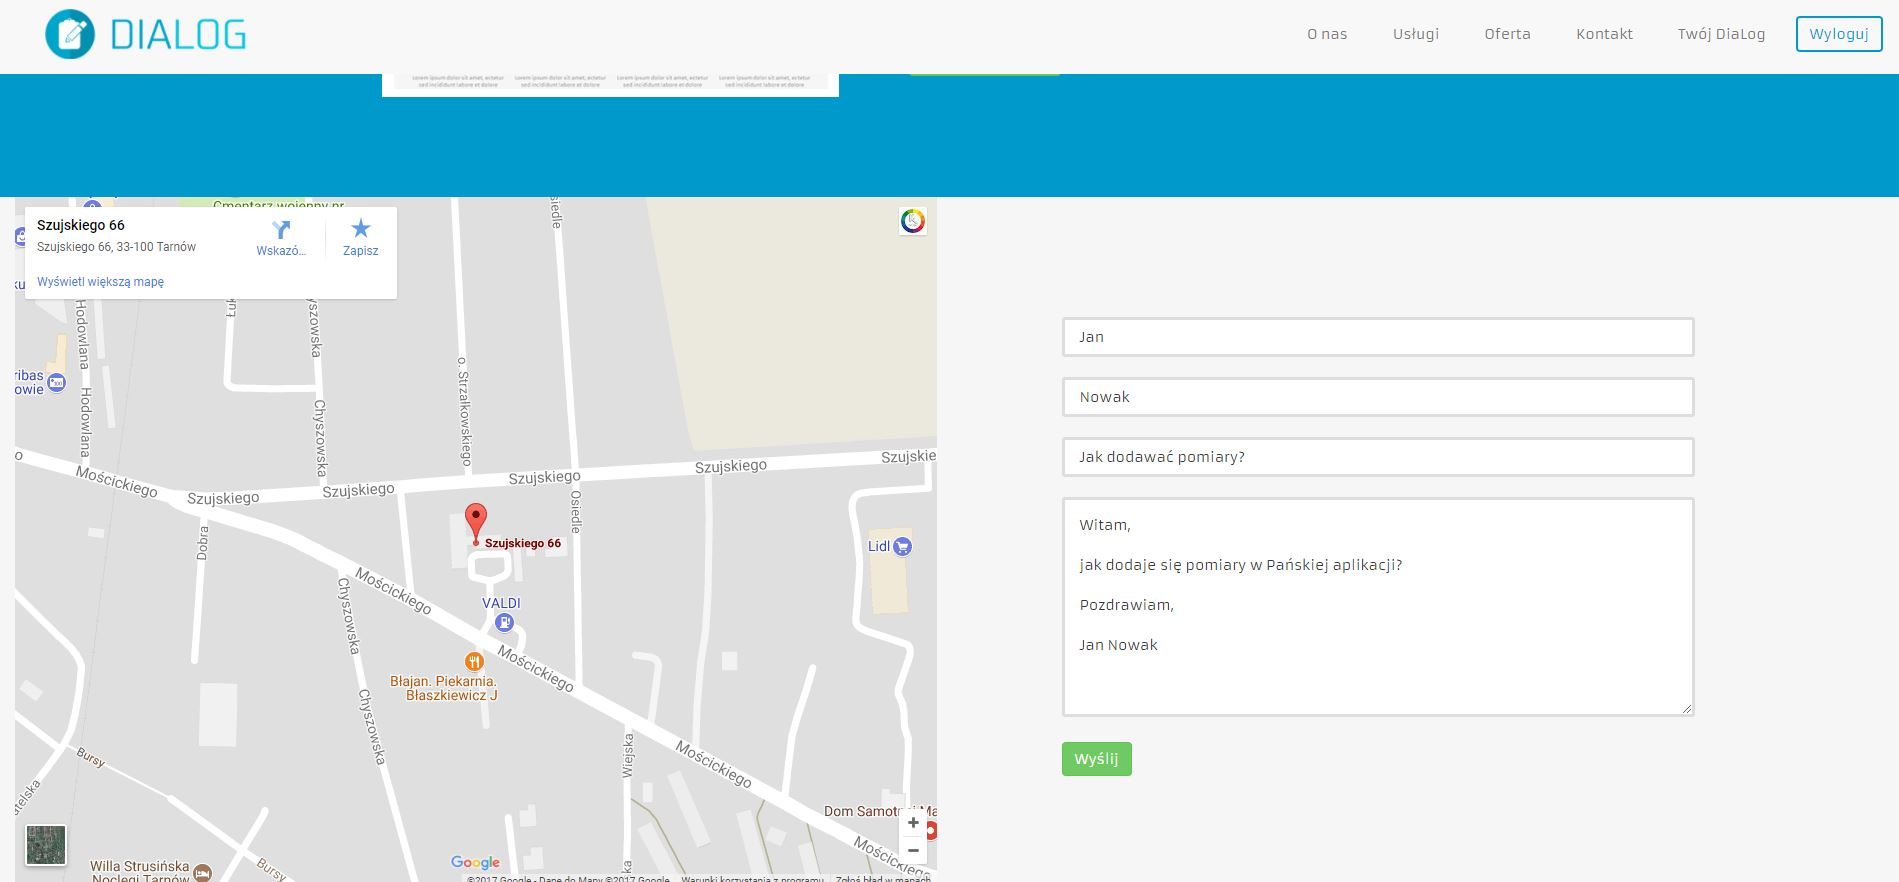
\includegraphics[scale=0.3]{images/email_module.jpg}
	\caption{Formularz do wysyłania maili do administracji}
	\label{Rys:email_module}
\end{figure}


\chapter{Bezpieczeństwo aplikacji}

Do przechowywania wrażliwych danych użytkownika, takich jak hasło wykorzystywane są mechanizmy oferowane przez usługodawcę \textit{Auth0}. Dane przechowywane w bazie tego serwisu nie mają postaci zwykłego tekstu, a przechowywane za pomocą skrótu \textit{BCrypt}.

\textit{BCrypt} jest funkcją skrótu kryptograficznego, która została stworzona w celu przechowywania haseł statycznych, czyli haseł znanych wyłącznie osobie, która chce się uwierzytelnać, a nie dowolnych danych binarnych. \textit{BCrypt} wymaga stosowania soli, co wyróżnia ją od innych funkcji skrótu. Sól w algorytmie \textit{BCrypt} jest złożona z nastepujących elementów:

\begin{itemize}
	\item \textit{version} oznaczające wersję algorytmu \textit{BCrypt},
	\item \textit{rounds} jest to liczba z przedziału 04-99, która określa tzw. \textit{work factor} algorytmu, domyślna wartość tego pola to \$12,
	\item \textit{saltaddon} -- są to losowe 22 znaki, które mają za zadanie powiększać sól weryfikacja tego ciągu przebiega przy użyciu wyrażenia regularnego [./A-Za-z0-9] -- znaki te mogą być wylosowane przez użytkownika, bądź przez specjalnie zaprojektowany do tego celu algorytm. 
\end{itemize}

W \textit{Auth0} zarówno dane \textit{REST-owe}, jak i przekazywane w ruchu sieciowym są szyfrowane. Cała komunikacja sieciowa wykorzystuje protokół TLS (\textit{Transport Layer Security}) w wersji 1.2 (będący rozwinięciem protokołu SSL), z co najmniej 128-bitowym szyfrowaniem AES (\textit{Advanced Encryption Standard}). Do wymiany kluczy wykorzystywany jest mechanizm \textit{ECDHE\_RSA} oparty na protokole \textit{Diffiego-Hellmana} z podpisem generowanym przy użyciu kryptograficznego algorytmu asymetrycznego RSA (\textit{Rivest–Shamir–Adleman}). 

Usługi świadczone przez serwis \textit{Auth0} zaprojektowane są z myślą o wysokiej dostępności i odporności. Aplikacje korzystające z \textit{Auth0} są częściowo zabezpieczone przed atakami typu \textit{Odmowa usługi} czy \textit{Uwierzytelnianie}. Mają one wbudowane funkcje ograniczania szybkości i automatycznego blokowania. Ponadto konta użytkowników zabezpieczone są za pomocą domyślnie wbudowanego modułu weryfikacji autentyczności użytkownika przy użyciu adresu e-mail. Każdy użytkownik systemu otrzymuje unikalny JWT (\textit{JSON Web Token}), który pozwala na rozróżnianie i sprawdzanie autentyczności użytkowników aplikacji. Aplikacja została zabezpieczona przed skopiowaniem linku do panelu użytkownika zalogowanego i wklejeniu go do innego okna przeglądarki w celu uzyskania dostępu. W~ momencie takiej próby użytkownik zostaje poinformowany, że nie ma uprawnień do przeglądania treści danej strony (rys. \ref{Rys:no_access}). 

\newpage

\begin{figure}[h]
	\centering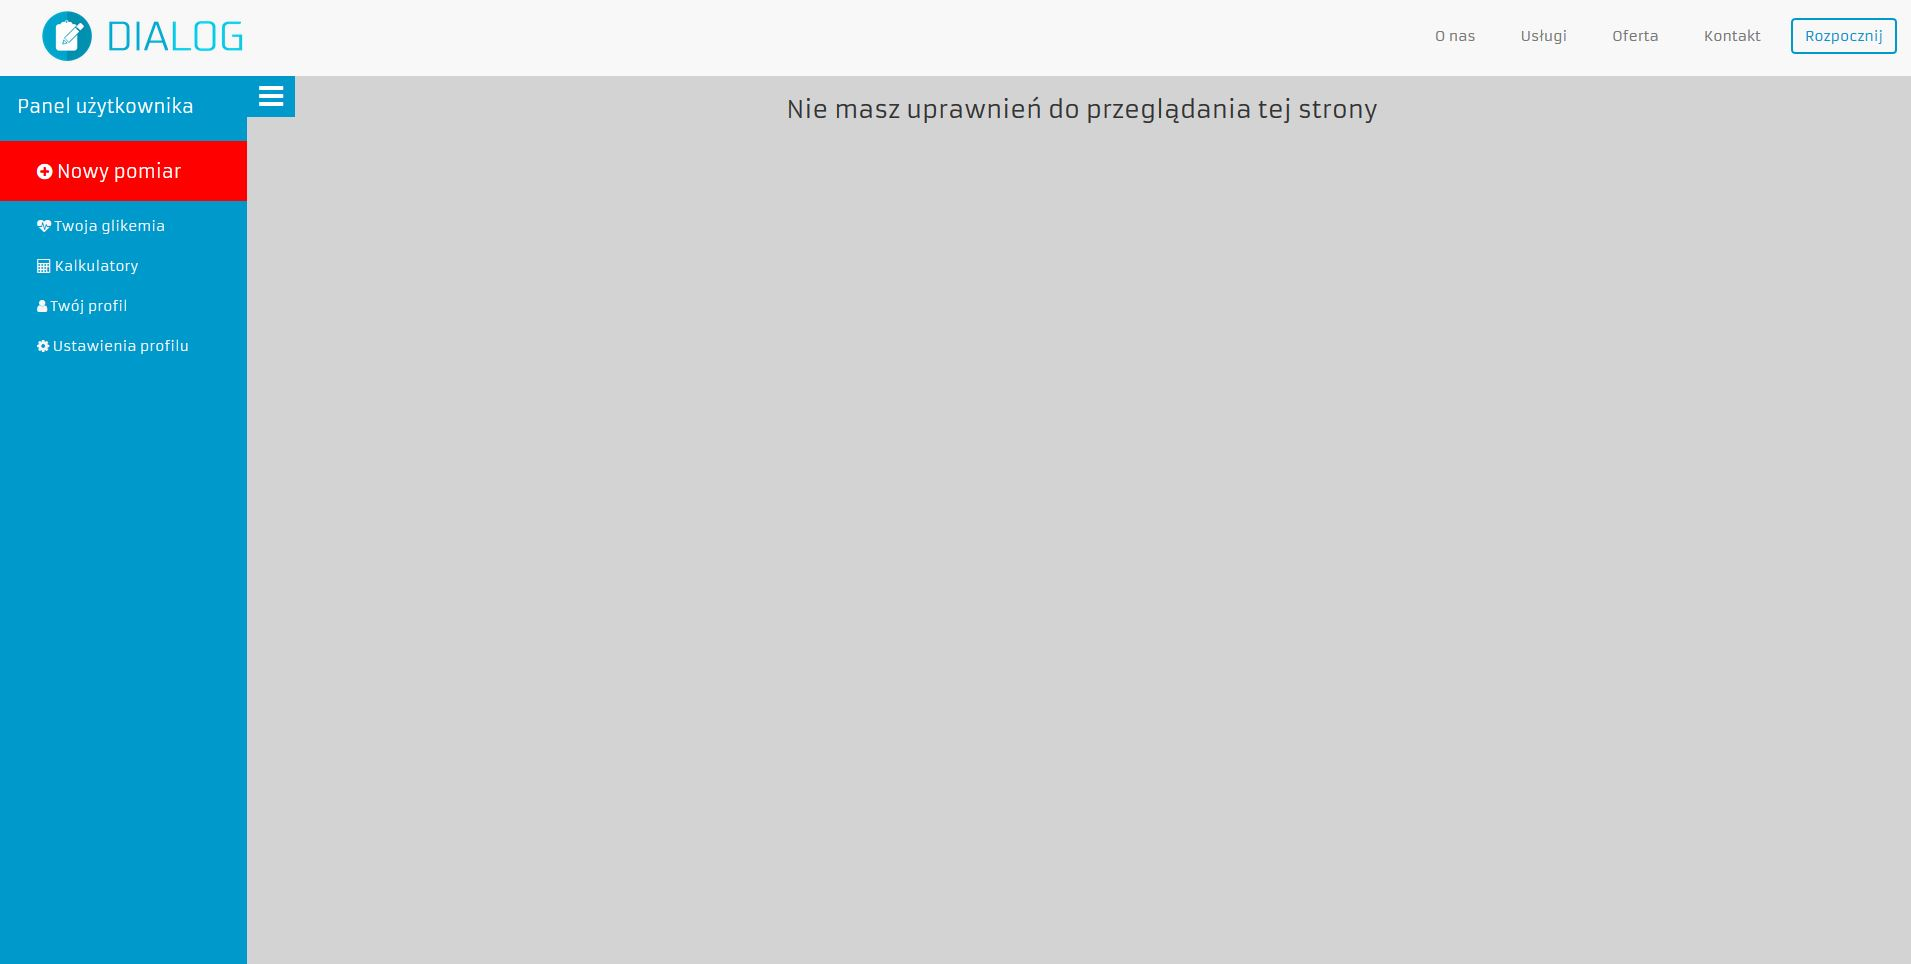
\includegraphics[scale=0.3]{images/no_access.jpg}
	\caption{Błąd przy próbie uzyskania dostępu do panelu użytkownika zalogowanego poprzez link URL}
	\label{Rys:no_access}
\end{figure}

Jak widać u góry (w menu górnym) nie ma dostępu do zakładki \textit{Twój dialog}, co oznacza, że użytkownik jest niezalogowany i próbuje uzyskać dostęp do linku URL udostępnianego wyłącznie użytkownikowi zalogowanemu. 

Podobna sytuacja tyczy się panelu administratora. Użytkownik nie posiadający w serwisie \textit{Auth0} roli \textit{Admin} nie posiada dostępu do funkcjonalności dla niej przeznaczonych. To oznacza, że nie da się uzyskać bezpośredniego dostępu do podstrony panelu administratora poprzez wklejenie linku URL do okna wyszukiwarki. Użytkownik przy takiej próbie zostaje natychmiastowo informowany właściwym komunikatem (rys. \ref{Rys:no_admin_access}).

\begin{figure}[h]
	\centering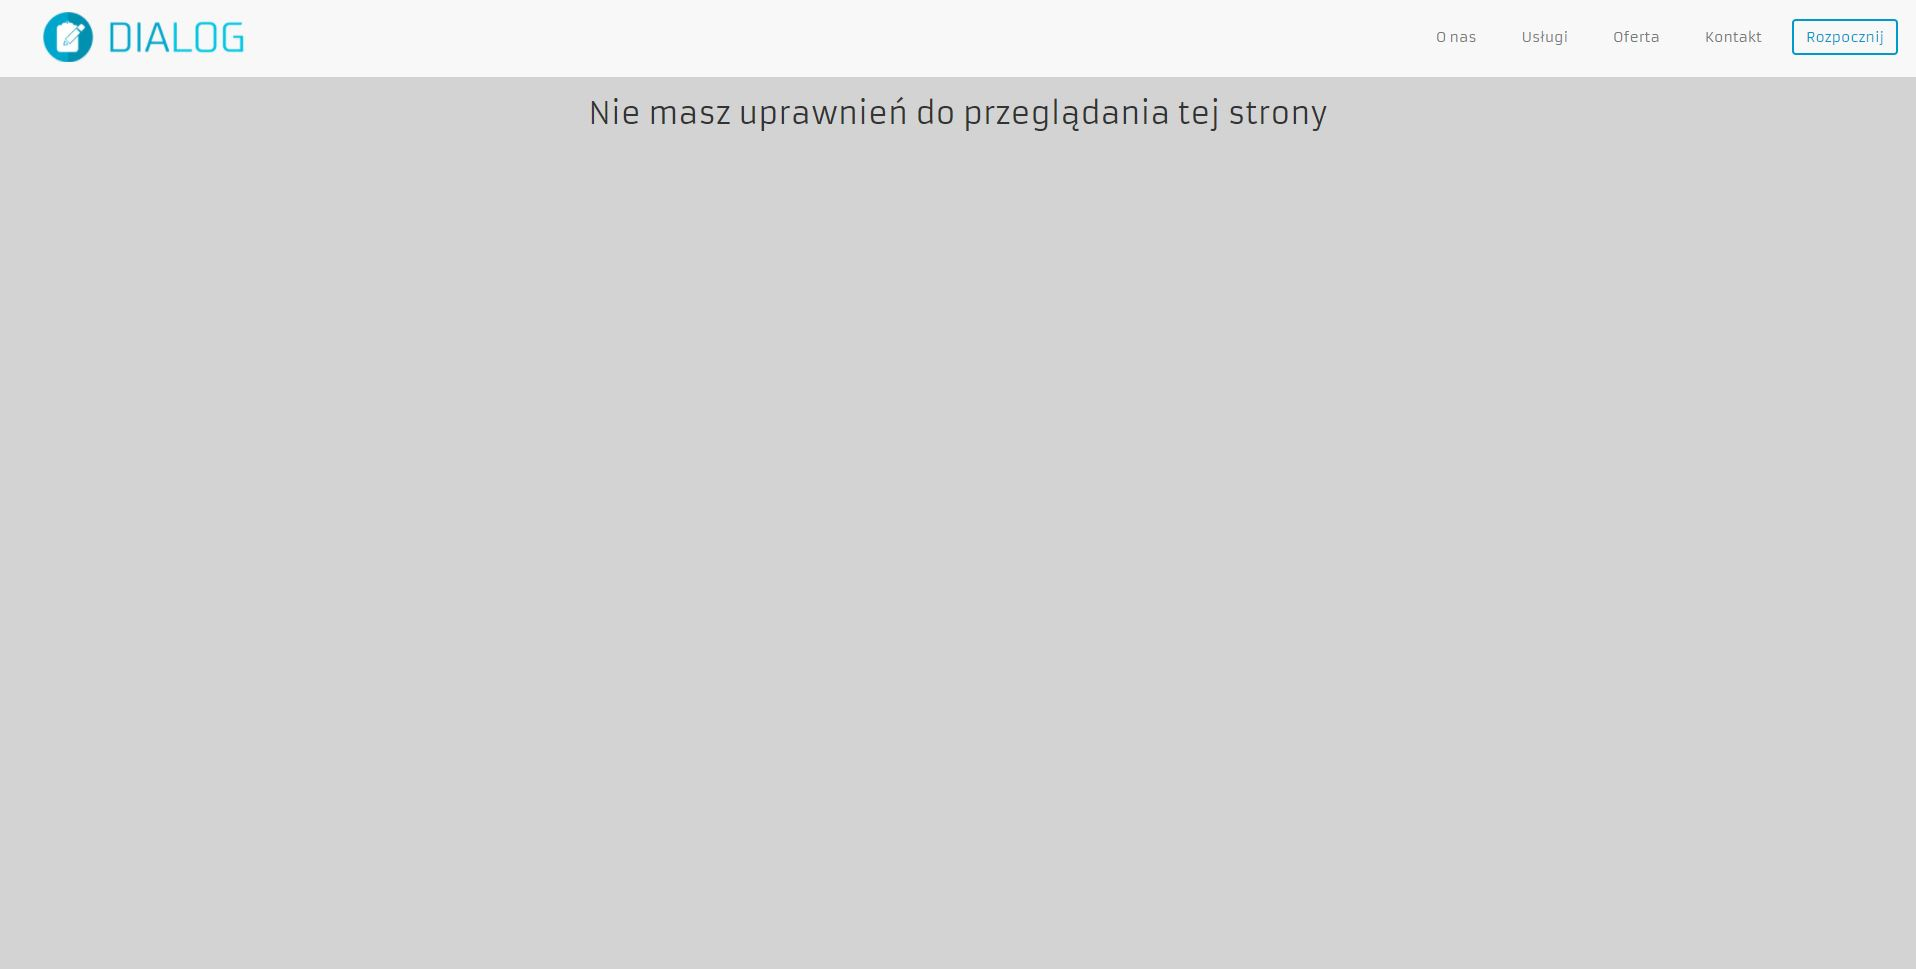
\includegraphics[scale=0.3]{images/no_admin_access.jpg}
	\caption{Błąd przy próbie uzyskania dostępu do panelu administratora poprzez link URL}
	\label{Rys:no_admin_access}
\end{figure}
\chapter{Testy}

\section{Debugowanie aplikacji i dostęp do informacji o jej działaniu}
Do wykonywania debugowania aplikacji w celu znalezienia błędów użyto wtyczki do programu \textit{Visual Studio Code} oraz wbudowanego w przeglądarkę internetową \textit{Google Chrome}, debuggera dostępnego z poziomu panelu narzędzi deweloperskich (zakładka \textit{Sources}) widoczna na rysunku \ref{Rys:sources} . W tym miejscu możliwe jest podejrzenie i debugowanie skryptów aplikacji. Programista ma również możliwość śledzenia wybranych wyrażeń (pole \textit{Watch expressions}), przeglądania stosu aplikacji (pole \textit{Call Stack}), ustawiania tzw. \textit{breakpointów} w momencie debugowania, przechodzenia kodu krok po kroku i wiele, wiele innych.

\begin{figure}[h]
	\centering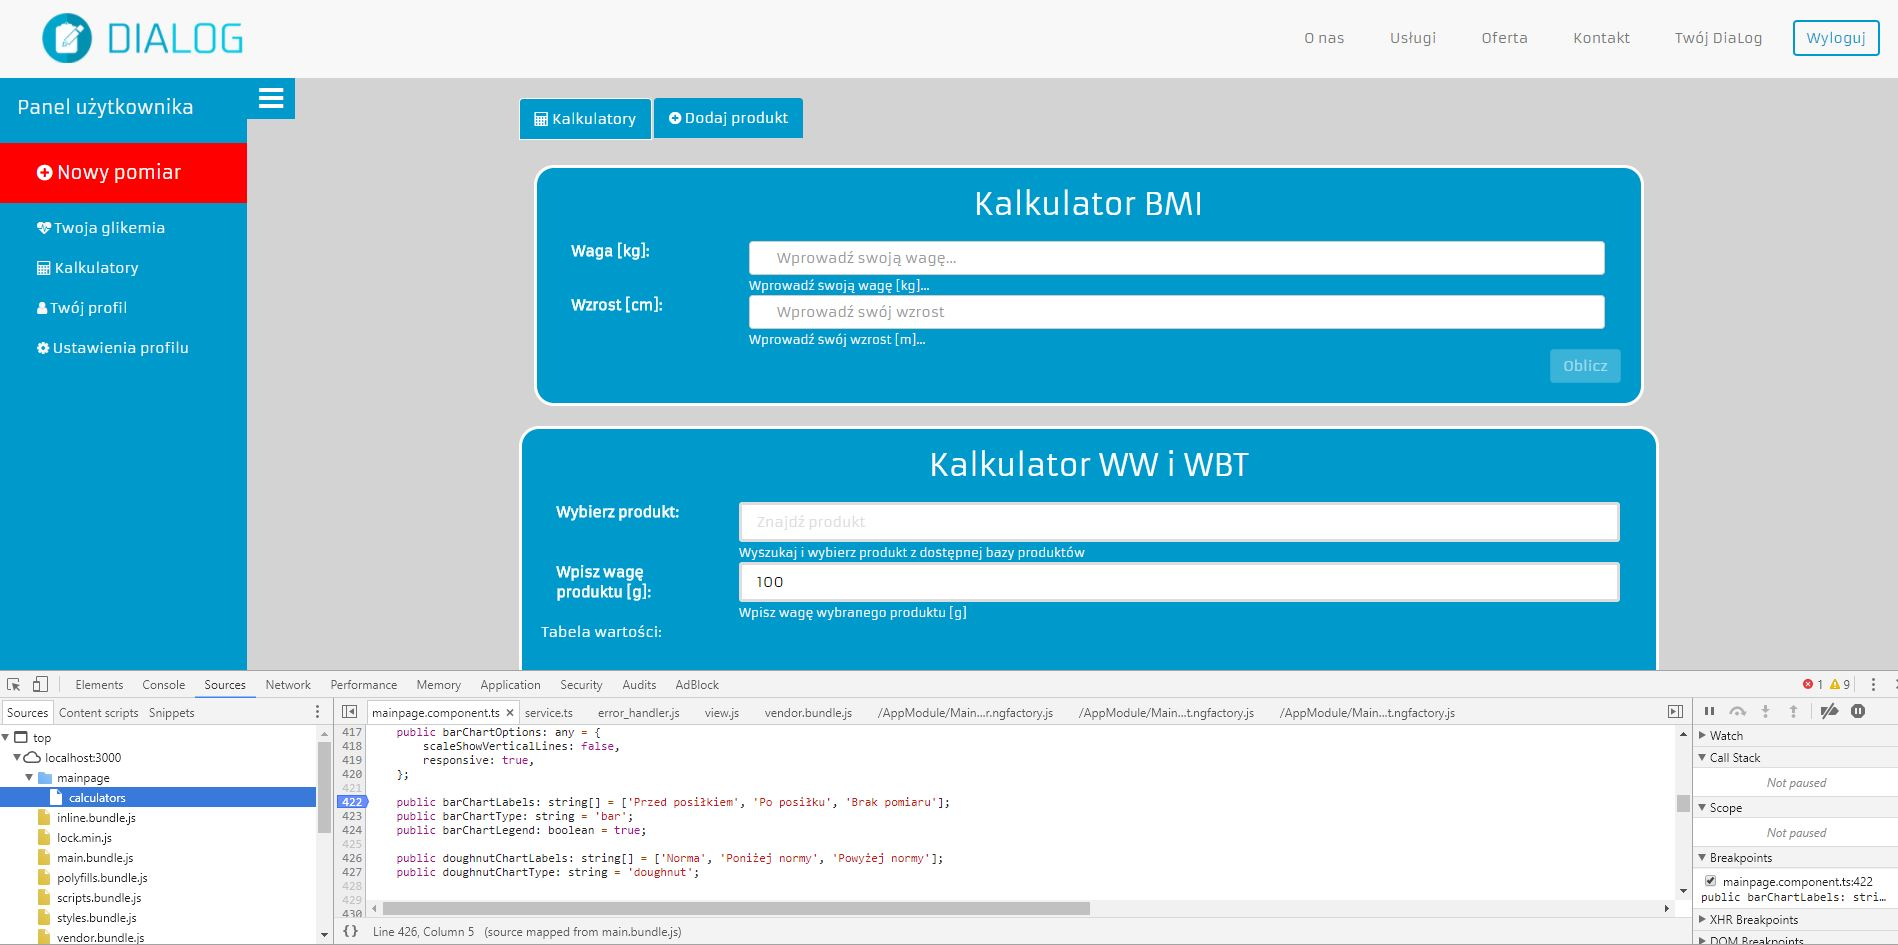
\includegraphics[scale=0.3]{images/sources.jpg}
	\caption{Opcje debugowania i podglądu kodu dostępne z poziomu zakładki \textit{Sources} narzędzi deweloperskich przeglądarki \textit{Google Chrome}}
	\label{Rys:sources}
\end{figure}


Do podglądu poprawności wysyłanych żądań za pomocą metod HTTP użyto narzędzi dostępnych z poziomu zakładki \textit{Network}. Oferuje ona podgląd adresów URL (\textit{Uniform Resource Locator}) generowanych do pobrania danych w formacie JSON oraz treści tablicy obiektu zawierającego te dane (rys. \ref{Rys:network}).
 
 \begin{figure}[h]
 	\centering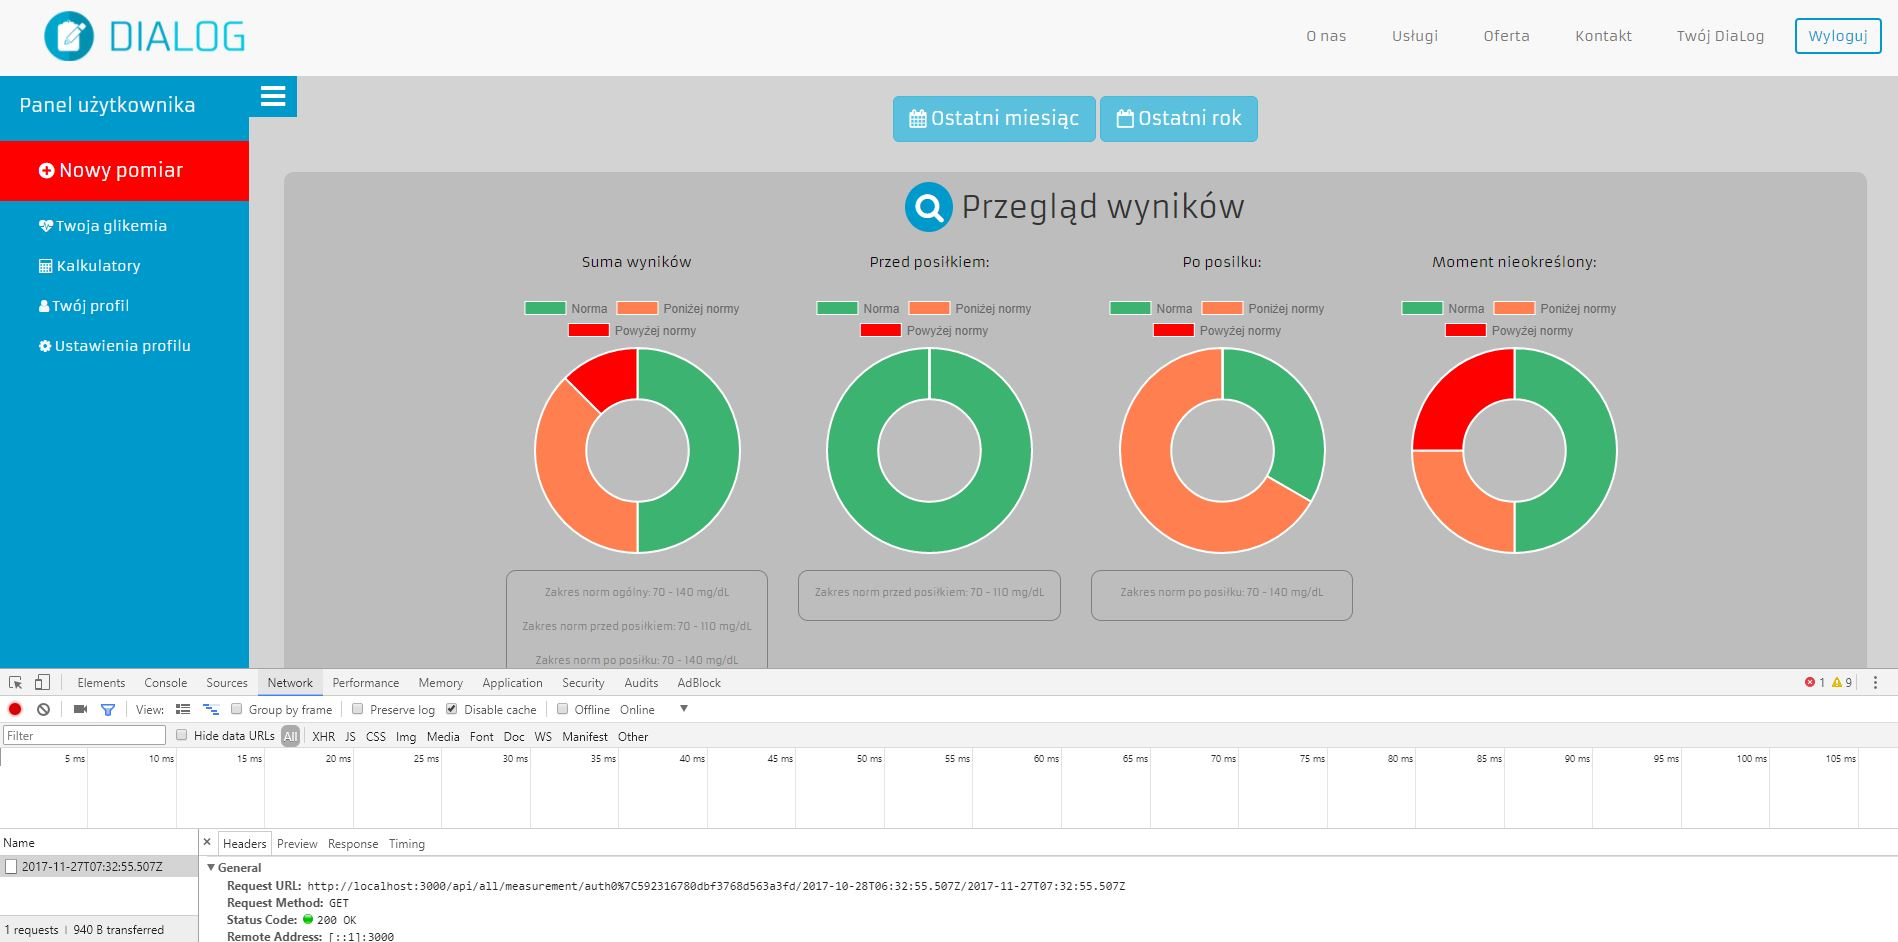
\includegraphics[scale=0.3]{images/network.jpg}
 	\caption{Opcje podglądu przesyłanych żądań dostępne z poziomu zakładki \textit{Network} narzędzi deweloperskich przeglądarki \textit{Google Chrome}}
 	\label{Rys:network}
 \end{figure}

\newpage
  
W celu identyfikacji rodzaju błędu posłużono się oknem konsoli dostępnym z poziomu zakładki \textit{Console}. Oferuje ona dokładny opis zaistniałego błędu wraz ze ścieżką lokalizacji do pliku z~ błędnym fragmentem kodu, a nawet numeru linijki, w której dany błąd wystąpił. W przypadku użycia metod HTTP (\textit{Hypertext Transfer Protocol}) wyświetlany jest odpowiedni numer błędu zgodnie ze specyfiacją kodów błędów HTTP. W oknie konsoli możliwy jest również podgląd wartości przechowywanych przez zmienne w projekcie oraz dostęp do treści ostrzeżeń w trakcie działania aplikacji (rys. \ref{Rys:console}).
 

 \begin{figure}[h]
	\centering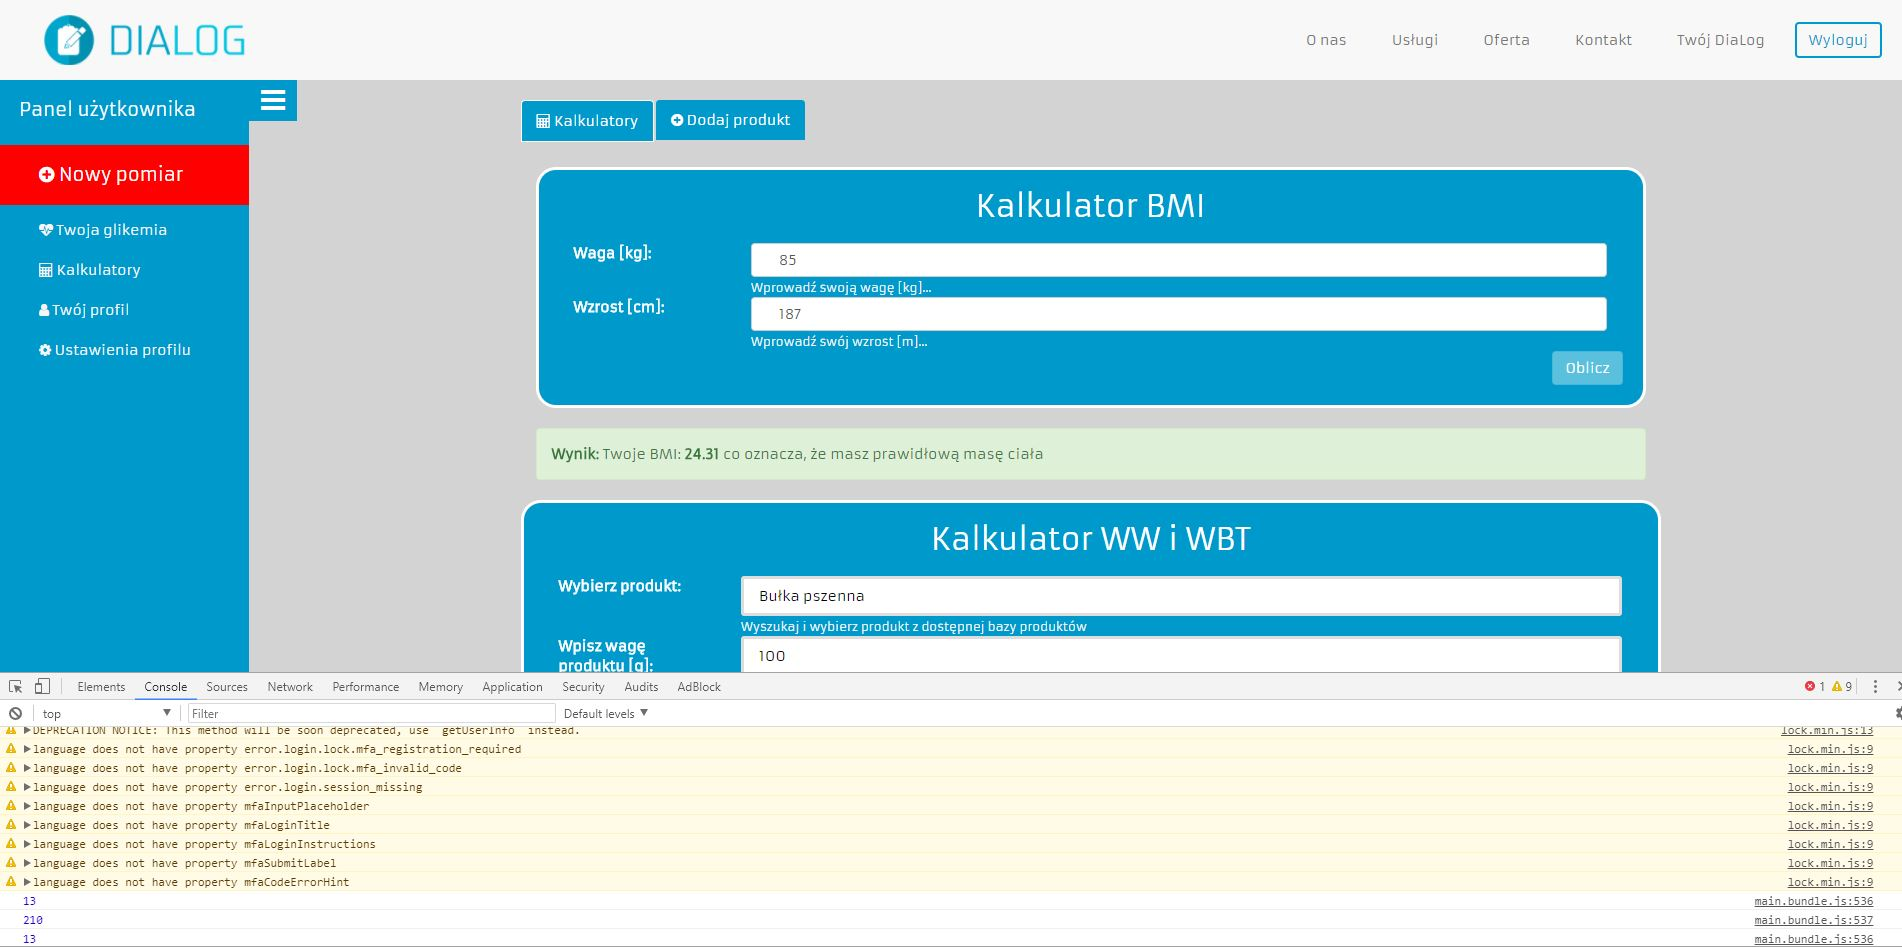
\includegraphics[scale=0.3]{images/console.jpg}
	\caption{Opcje podglądu błędów, ostrzeżeń i wartości zmiennych dostępne z poziomu zakładki \textit{Console} narzędzi deweloperskich przeglądarki \textit{Google Chrome}}
	\label{Rys:console}
 \end{figure}

\section{Testy funkcjonalne aplikacji}

Aplikację skonstruowano pod kątem UX (\textit{User Experience}), a kod napisano w~ oparciu o podstawowe zasady budowania struktury projektu tworzonego z wykorzystaniem frameworku \textit{Angular 2} \cite{Ans}. Dołożono wszelkich starań, aby ilość danych umieszczanych w~ ramach jednego widoku nie była zbyt duża, ponieważ w~ przypadku \textit{Angulara 2} znacząco obniża to wydajność aplikacji. 

W ramach testów funkcjonalnych aplikacji przeprowadzono podstawowe czynności mające na celu zapewnienie stabilności jej działania. Zostały one wykonane zgodnie z założeniami funkcjonalnymi, jakie powinien spełniać program. Pierwszym krokiem było sprawdzenie poprawności wysyłanych do serwera żądań (\textit{Requests}) w celu pobrania danych (\textit{Response Data}). Posłużono się oprogramowaniem \textit{Postman}. 

Każda z metod HTTP (\textit{Hypertext Transfer Protocol}) służących do komunikacji z serwerem w celu pobrania lub wysłania danych została sprawdzona poprzez wprowadzenie najpierw błędnych, a następnie poprawnych parametrów w nagłówku, bądź w adresie URL (\textit{Uniform Resource Locator}) metody. Przykładowe wyniki testu przedstawiono na rysunkach \ref{Rys:postman_fail} oraz \ref{Rys:postman_good}.

\begin{figure}[h]
	\centering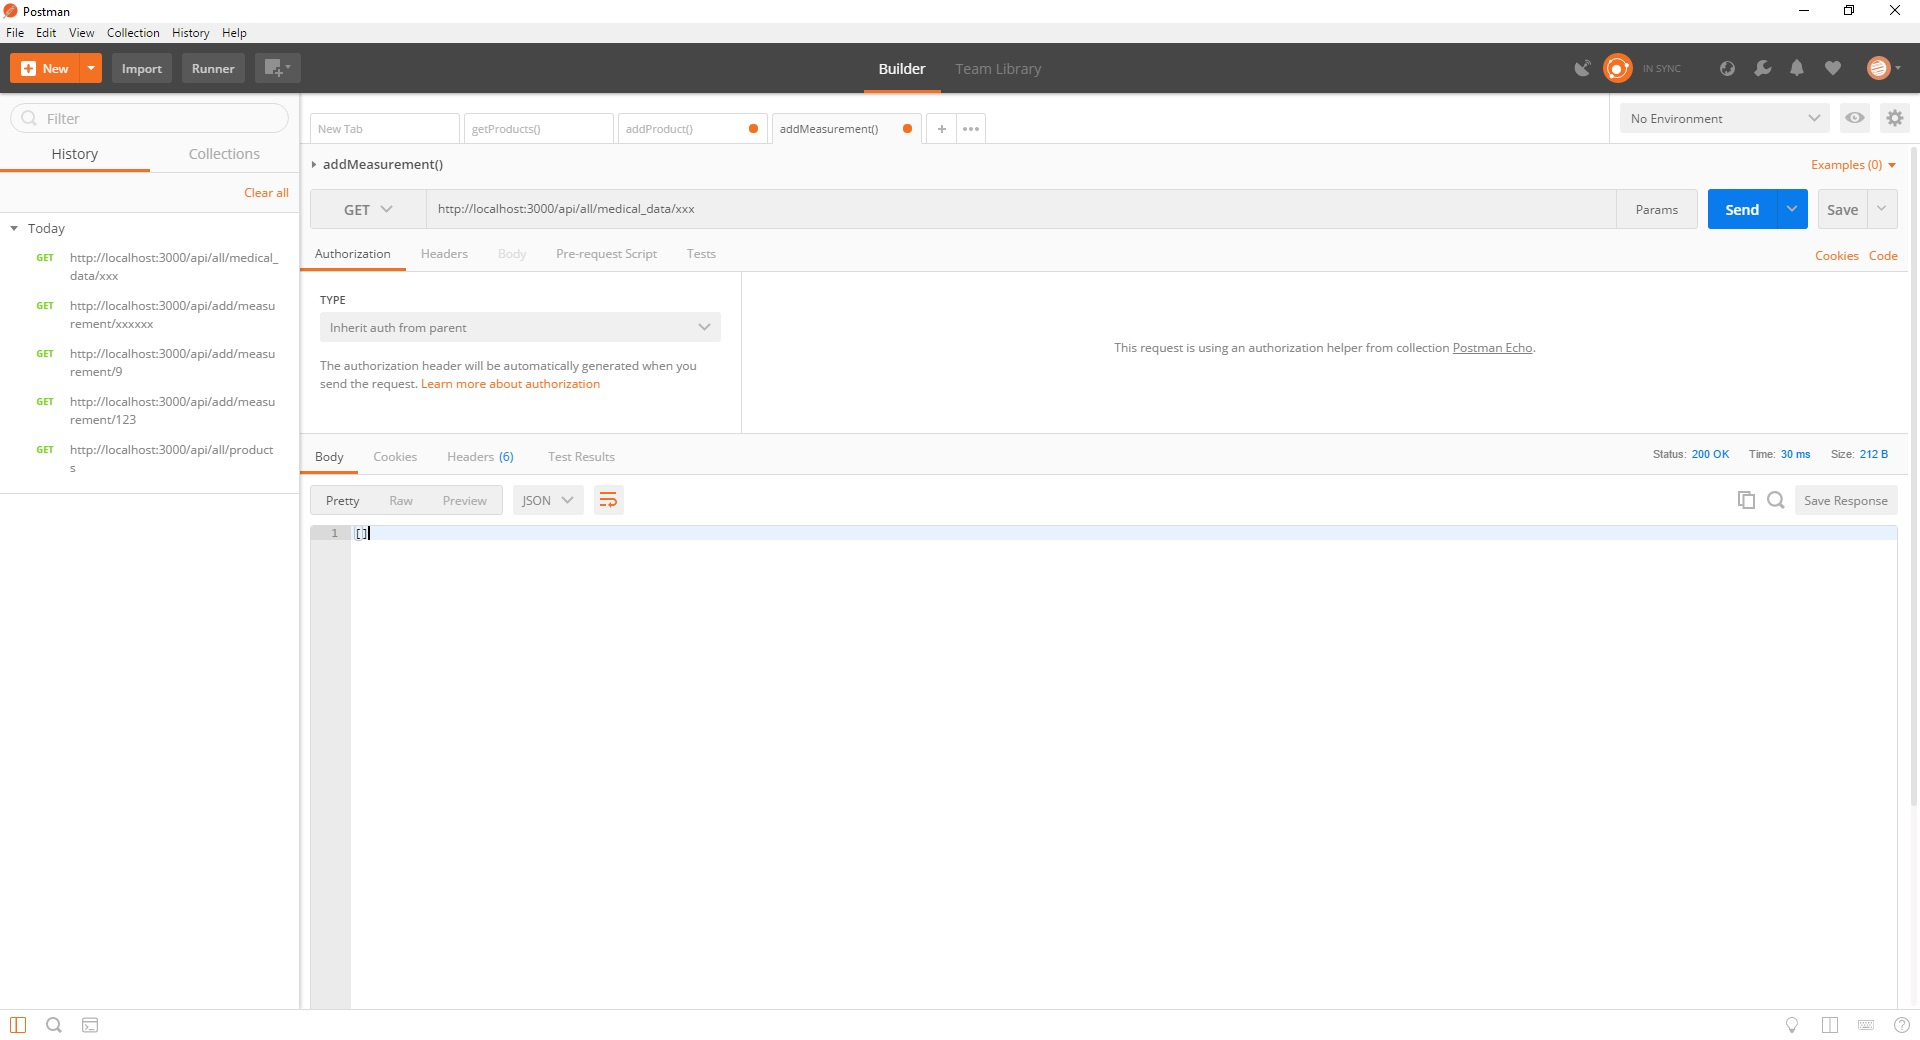
\includegraphics[scale=0.3]{images/postman.JPG}
	\caption{Próba pobrania danych medycznych za pomocą oprogramowania \textit{Postman} użytkownika o błędnym identyfikatorze}
	\label{Rys:postman_fail}
\end{figure}

W przypadku wprowadzenia błędnego identyfikatora użytkownika w adresie URL metody GET służącej do pobrania jego danych medycznych uzyskano odpowiedź z serwera z pustą tablicą danych. 

Przy próbie wprowadzenia poprawnego identyfikatora w adresie URL tej samej metody serwer zwrócił żądane dane medyczne użytkownika.

\newpage

\begin{figure}[h]
	\centering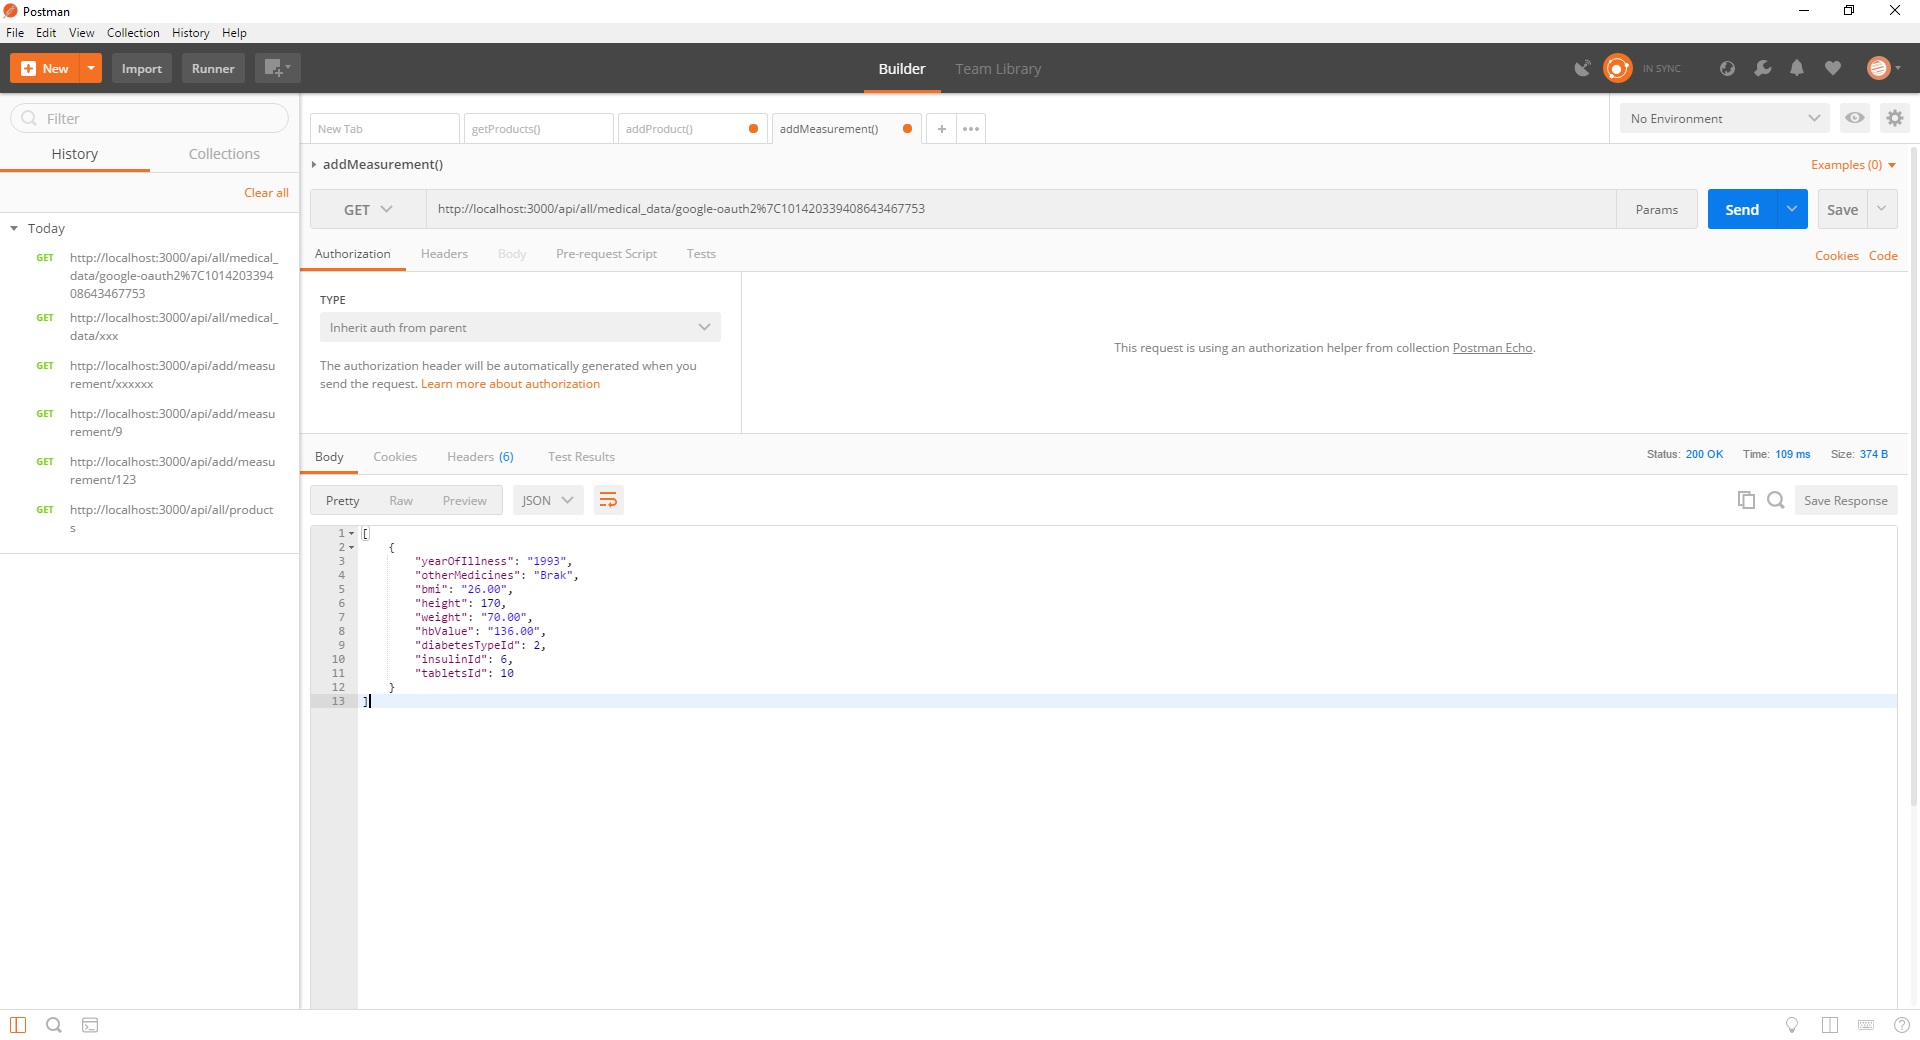
\includegraphics[scale=0.3]{images/postman2.JPG}
	\caption{Próba pobrania danych medycznych za pomocą oprogramowania \textit{Postman} użytkownika o poprawnym identyfikatorze}
	\label{Rys:postman_good}
\end{figure}

Kolejną czynnością było sprawdzenie poprawności walidacji danych w formularzach aplikacji. Reguły walidacji odpowiednich pól określone zostały przy użyciu wyrażeń regularnych. Zastosowano odpowiedni przycisk powiązany bezpośrednio z formularzem, służący do wysyłania żądania z uzupełnionymi danymi. Zablokowano go do momentu kiedy użytkownik nie wprowadzi poprawnych danych. Takie podejście zabezpiecza program przed błędami związanymi z niezgodnością typów w bazie danych. Pozwala również uniknąć zapisywania informacji (takich jak kod pocztowy) w niewłaściwym formacie (rys. \ref{Rys:form}) \cite{Ang}. 
  
\begin{figure}[h]
	\centering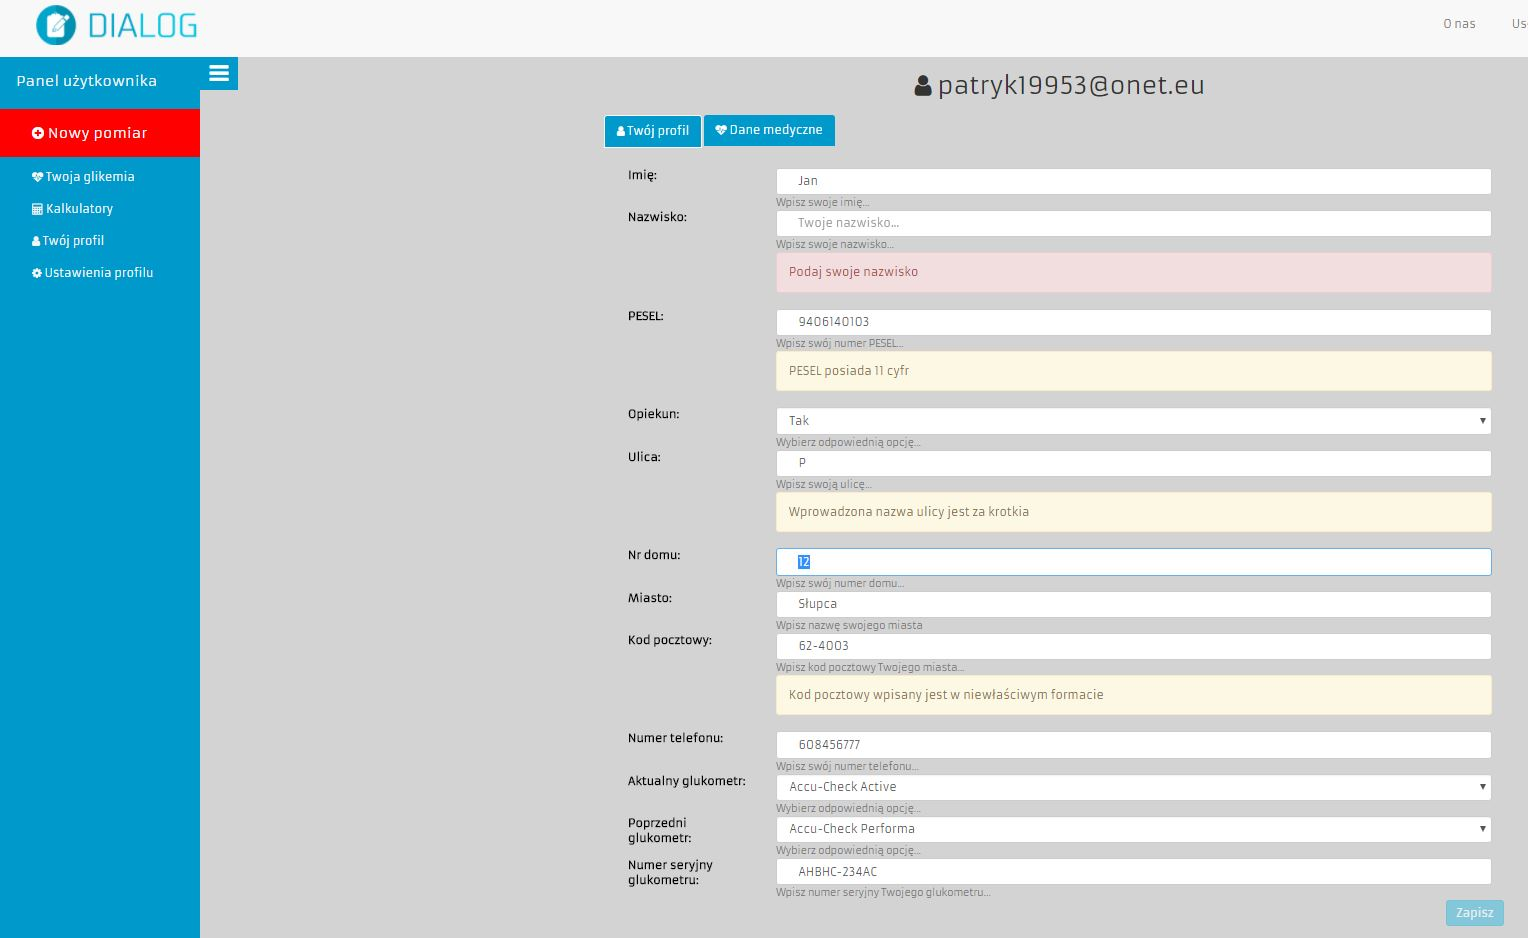
\includegraphics[scale=0.35]{images/form.JPG}
	\caption{Widok formularza z błędnie wypełnionymi polami i zablokowanym przyciskiem do zapisu ich wartości}
	\label{Rys:form}
\end{figure}




\chapter{Zakończenie}

Ustosunkowując się do założeń podanych we wstępie pracy, dołożono wszelkich starań, aby oferowane przez aplikacje funkcjonalności działały zgodnie z ich przeznaczeniem oraz zaprezentowane były za pomocą prostego i przejrzystego interfejsu. Aplikacja ma być jedynie jednym z~ czynników przyczyniających się do postępów w leczeniu cukrzycy. 

Poprzez oferowanie czytelnych wykresów podsumowujących wszystkie, dotychczasowe pomiary wprowadzone przez użytkownika oraz tabeli zestawień grupującej wartości pomiarów osoba korzystająca z aplikacji wyciągać ma poglądowe wnioski na temat tego jak przebiega jej choroba od momentu założenia konta w systemie. Ponadto, dzięki dostępnym kalkulatorom BMI (\textit{Body Mass Index}), wymienników węglowodanowych czy wymienników białkowo-tłuszczowych opartych na stale rozwijanej przez użytkowników bazie produktów i danych wprowadzanych przez korzystającą z nich osobę możliwe jest określenie jaki stopień współczynnika masy ciała posiada dany użytkownik czy też jakie produkty mogą być spożyte w danej chwili tak, aby nie zakłócić porządku dziennej diety i nie pogłębić stopnia zaawansowania cukrzycy. 

Jeżeli chodzi o dalsze etapy rozwoju aplikacji -- autor chciałby rozszerzyć jej funkcjonalność o~ moduł oparty na zdobywaniu punktów przez użytkowników w zamian za postępy w leczeniu cukrzycy. Funkcjonalność ta mogłaby mieć znaczący wpływ na motywację i~ sukcesywne korzystanie z aplikacji w zamian za systematyczne prowadzenie pomiarów. Dodatkowo, jest w~ planach dodanie modułu skanowania kodów kreskowych produktów przez użytkowników za pomocą kamerki internetowej, bądź kamery telefonu i~ automatycznego dodawania ich do bazy danych systemu. Ułatwiłoby to znacznąco proces wprowadzania nowego produktu.



% Bibliography (books, articles) starts here.
\bibliographystyle{plalpha}{\raggedright\small\bibliography{bibliography}}

\cleardoublepage\appendix%
\chapter{Załączniki}

Płyta CD z następującą zawartością:
\begin{itemize}
	\item tekst pracy w formacie PDF,
	\item projekt z plikami źródłowymi.
\end{itemize}


\end{document}
